\documentclass[11pt]{article}
\title{\vspace{-2cm}Quals Study Guide}
\author{Mackenzie Lau}
\date{}
\usepackage[margin = 0.75in]{geometry}
\usepackage{graphicx, subcaption, wrapfig, epstopdf}
\usepackage{amsmath, amssymb, gensymb, tabularx, multirow, esint, indentfirst}
\usepackage{mathtools, bm, enumitem}
\usepackage[utf8]{inputenc}
\usepackage[super]{nth}
\usepackage[hidelinks]{hyperref}
\newcommand{\Hrule}{\rule{\textwidth}{0.2mm}\\}
\newcommand{\Item}[1]{\item \textbf{#1}:}
\newcommand{\Header}[1]{\noindent\rule{\textwidth}{0.4pt}\\[0.3cm]\indent \large{\textit{#1}}\normalsize{}\\[-0.1cm]\noindent\rule{\textwidth}{0.4pt}}
\newcommand{\CenteredBoxed}[1]{\begin{center}\boxed{#1}\end{center}}
\newcommand{\sumlim}[2]{\sum\limits_{#1}^{#2}}
\newcommand{\intlim}[2]{\int\limits_{#1}^{#2}}
\usepackage [english]{babel}
\usepackage [autostyle, english = american]{csquotes}
\MakeOuterQuote{"}
\newsavebox{\fmbox}
\newenvironment{fmpage}[1]{\begin{lrbox}{\fmbox}\begin{minipage}{#1}}{\end{minipage}\end{lrbox}\fbox{\usebox{\fmbox}}}
%% Aero commands
\newcommand{\rhoinfty}{\rho_\infty}
\newcommand{\Vinfty}{V_\infty}
\newcommand{\qinfty}{q_\infty}
\newcommand{\TSL}{T_{SL}}
\newcommand{\WTO}{W_{TO}}
%% Optimization commands
\newcommand{\boldx}{\mathbf{x}}
\newcommand{\xstar}{\boldx^*}
\newcommand{\Partial}[2]{\frac{\partial #1}{\partial #2}}
\newcommand{\PPartial}[2]{\frac{\partial^2 #1}{\partial #2^2}}
\newcommand{\PPPartial}[3]{\frac{\partial^2 #1}{\partial #2 \partial #3}}
\DeclareMathOperator{\Hessian}{Hess}
%% Thermodynamics commands
\newcommand{\PartialConst}[3]{\left(\Partial{#1}{#2}\right)_{#3}}
\newcommand{\Problem}[1]{\Item{Problem #1}}
%% Combustion commands

\begin{document}
\maketitle
\thispagestyle{empty}
\vspace{-1cm}
\Hrule
\vspace{-1cm}
\pagestyle{empty}
\tableofcontents
\newpage
\pagestyle{plain}
\setcounter{page}{1}
\section{Fixed Wing Design}
\subsection{Basics and Background}
\begin{itemize}
\Item{Requirements Definition} A statement which identifies a system, product, or process characteristic of constraint which is unambiguous, can be verified, and is deemed necessary for stakeholder acceptability. Well-formed requirements include system functionality (capability), attributes (measurable conditions), and are bounded by constraints.
\Item{Requirement Analysis} Transform identified top-level needs and objectives into system function and performance requirements which specifically define what the system must do, how well it must perform, and what must be accomplished to ensure operational capabilities with interfacing systems are met.
\Item{What Are Requirements?} Precise statements of what must be done as well as how well and under what conditions it must be done. Delineated by the "Three C's": Capabilities, Characteristics, and Constraints.
\Item{Constraint Analysis} Ensure system can satisfy all constraints set by requirements (sizing procedure).
\Item{Mission Analysis} Analyzing system performance over a given mission (sizing procedure).
\Item{Energy-/Power-Based Analysis} Constraint diagram (carpet plot).
\Item{Layers of the Atmosphere}
	\begin{itemize}
	\Item{Troposphere} Up to 8 to 14.5 km (5 to 9 miles). Most dense, contains all weather.
	\Item{Stratosphere} Up to 50 km (31 miles). Ozone layer absorbs and scatters UV radiation.
	\Item{Mesosphere} Up to 85 km (53 miles). Meteors burn up here.
	\Item{Thermosphere} Up to 600 km (372 miles). Satellites orbit here.
	\Item{Ionosphere} Overlaps mesosphere and thermosphere, 48 to 965 km (30 to 600 miles). Makes radio communication possible.
	\Item{Exosphere} Up to 10,000 km (6,200 miles). Upper limit of atmosphere.
	\end{itemize}
\Item{Standard Atmosphere} 66.2\degree F (19\degree C), 1.075 atm (108.9 kPa), 0.0025195 $slug/ft^3$ (1.2985 $kg/m^3$)
\Item{Temperature Lapse} Troposphere: approx -18.8\degree F per mile (-6.5\degree C per km). Stratosphere: approx. +2.89\degree F per mile (+1.0\degree C per km)
\end{itemize}

\subsection{Aerodynamics}
\subsubsection{Fundamentals of Fluid Dynamics}
\begin{itemize}
\Item{Inviscid Flow} Zero viscosity ($Re = \infty$)
\Item{Incompressible Flow} Constant density
\Item{Bernoulli's Equation} $p + \frac{1}{2}\rho V^2 = const.$\\
	\begin{itemize}
	\item Start from general momentum equation $\rho\frac{Du}{Dt} = \sum F''' = -\frac{\partial p}{\partial x}+ \rho f_x + f_v$, ignoring body and viscous forces. Assume, without loss of generality, we are in the $x$ direction
	\item Write out substantial derivative $\rho\frac{Du}{Dt} = \rho\left(\frac{\partial u}{\partial t} + u\frac{\partial u}{\partial x} + v\frac{\partial u}{\partial y} + w\frac{\partial u}{\partial z}\right)$. Assuming steady flow $\frac{\partial u}{\partial t} = 0$
	\item Substitute, multiply both sides by $dx$, and simplify by applying to a stream (such that $udz=wdx$ and $udy=vdx$) to get $u\left(\frac{\partial u}{\partial x}dx+\frac{\partial u}{\partial y}dy+\frac{\partial u}{\partial z}dz\right)=\frac{-1}{\rho}\frac{\partial p}{\partial x}dx$
	\item Recognize the term in parentheses on the left hand side is the differential of the $x$-component of the velocity $du = \frac{\partial u}{\partial x}dx+\frac{\partial u}{\partial y}dy+\frac{\partial u}{\partial z}dz$
	\item Substitute to get $udu = \frac{-1}{\rho}\frac{\partial p}{\partial x}dx$
	\item Repeat for $y$ and $z$ directions
	\item Recognize the sum of squares of the velocity components is the square of the velocity itself ($u^2+v^2+w^2=V^2$)
	\item Recognize the sum of the partial derivatives of pressure in each direction multiplied by the component differential is the differential of the pressure ($\sum\frac{\partial p}{\partial x_i}dx_i = dp$)
	\item Arrive at Euler's equation: $\frac{1}{2}d(V^2) = \frac{-dp}{\rho}\implies$ \boxed{dp = -\rho VdV}. Euler's equation applies to \textit{any} steadily flowing fluid
	\item Apply Euler's equation to a streamline assuming constant density (incompressible flow) and integrate between two states to get Bernoulli's equation 
	$$\intlim{p_1}{p_2}dp = -\rho\intlim{V_1}{V_2}VdV$$
	$$p_2-p_1 = \rho\left(\frac{1}{2}V_1^2 - \frac{1}{2}V_2^2\right)$$
	$$p_1 + \frac{1}{2}\rho V_1^2 = p_2 + \frac{1}{2}\rho V_2^2$$
	\CenteredBoxed{p+\frac{1}{2}\rho V^2 = const.}
	\item Bernoulli's equation applies to any individual stream line, indepent of whether or not the flow is rotational. In the special case of irrotational flow ($\nabla\times V = 0$) the constant is the same for each streamline, thus Bernoulli's equation holds for the entire flow field, not just a streamline.
	\end{itemize}
\Item{Irrotational Flow} A flow is irrotational if individual fluid elements do not rotate about their centers of gravity; the fluid elements posses no angular velocity and their motion through space is pure translation ($\nabla\times V = 0$ throughout the fluid). Inviscid flow may be either rotational or irrotational. Viscous flow must be rotational, thus all \emph{real} flows are rotational; irrotational flow is an idealization used to simplify analyses.
\Item{Circulation} $\Gamma\equiv-\oint V\cdot ds=\varointclockwise V\cdot ds$ (circulation is taken to be positive clockwise for convenience). Circulation does \emph{not} imply the fluid elements are doing circuits; rather, circulation in the context of aerodynamics means the closed-loop integral is finite. Applying Stoke's theorem yields $-\frac{d\Gamma}{dS} = (\nabla\times V)\cdot\mathbf{n}$ where $\mathbf{n}$ is the normal to the open surface which bounds the curve around which $V\cdot ds$ is integrated.
\Item{Stream Function} Two-dimensional steady flow yields the equation $\frac{dy}{dx} = \frac{v}{u}$ for a streamline. With $v$ and $u$ known functions of $x$ and $y$, we can write the stream function $\bar{\psi}(x,y) = c$
	\begin{itemize}
	\item Since the velocity vector at any point is tangent to the stream line at that point (i.e. there is no normal velocity) the mass flux between any two stream lines must remain constant throughout the flow field (for incompressible flow). This means local velocity is inversely proportional to stream line spacing at any point in the flow
	\item We can also deduce the following
	$$ \Delta\bar{\psi}\equiv\rho V\Delta n(unit\ depth\ into\ page)$$
	$$\lim_{\Delta n\to0}\frac{\Delta\bar{\psi}}{\Delta n}\equiv\Partial{\bar\psi}{n} = \rho V$$
	$$\textrm{Conservation of mass}\implies\rho V\Delta n = \rho u\Delta y - \rho v\Delta x$$
	$$d\bar{\psi} = \rho udy - \rho vdx$$
	$$\textrm{By the chain rule}\ \bar{\psi} = \bar{\psi}(x,y) \implies d\bar{\psi} = \Partial{\bar\psi}{x}dx + \Partial{\bar\psi}{y}dy$$
	\CenteredBoxed{\rho u = \Partial{\bar\psi}{y}\to u=\Partial{\psi}{y},\quad \rho v = -\Partial{\bar\psi}{x}\to v=-\Partial{\psi}{x}}
	\item Polar coordinates: $u_r=\frac{1}{r}\Partial{\psi}{\theta}$, $u_\theta=-\Partial{\psi}{r}$
	\end{itemize}
\Item{Velocity Potential} If $\xi = \nabla\times V = 0$ then $\exists\phi=\phi(x,y,z):\mathbb{R}^3\to\mathbb{R}\ s.t.\ \nabla\times(\nabla\phi)=0$ and $V=\nabla\phi$
	\begin{itemize}
	\item As a direct consequence, $u=\Partial{\phi}{x}$, $v=\Partial{\phi}{y}$, $w=\Partial{\phi}{z}$ (from definition of Cartesian gradient)
	\item Cylindrical coordinates: $u_r=\Partial{\phi}{r}$, $u_\theta=\frac{1}{r}\Partial{\phi}{\theta}$, $u_z=\Partial{\phi}{z}$
	\item Spherical coordinates: $u_r=\Partial{\phi}{r}$, $u_\theta=\frac{1}{r}\Partial{\phi}{\theta}$, $u_\Phi=\frac{1}{r\sin\theta}\Partial{\phi}{\Phi}$, 
	\end{itemize}
\Item{Vortex Sheet Strength} $\Gamma = \intlim{a}{b}\gamma ds$
	\begin{itemize}
	\item Local vortex strength is equal to the local velocity discontinuity ($\gamma=u_1-u_2$)
	\item Kutta-Joukowski Theorem: $L' = \rhoinfty \Vinfty\Gamma$
	\item Kutta Condition $\implies (\gamma(TE) = 0)\ ||\ (\gamma(TE) = \mathrm{finite}\implies V_1=V_2\neq0)$
	\item Kelvin's Circulation Theorem: $\frac{D\Gamma}{Dt} = 0$, i.e. in inviscid, incompressible flow, the circulation around a closed curve consisting of the same fluid elements does not change with time. This leads to the starting and shed vortex theories.
	\end{itemize}
\end{itemize}
\subsubsection{Two-Dimensional Aerodynamics}
\Header{Fundamentals}
\begin{itemize}
\Item{Purpose of an Airfoil} Generate lift
\Item{Draw an Airfoil}
\Item{NACA 4 Series} 
	\begin{itemize}
	\item \nth{1} = max camber as percent of chord
	\item \nth{2} = location of max camber as percent of chord
	\item \nth{3}-\nth{4} = max thickness as percent of chord
	\end{itemize}
\Item{NACA 5 Series}
	\begin{itemize}
	\item \nth{1} = two-thirds design $c_l$, in tenths
	\item \nth{2} = location of max camber, in fifths
	\item \nth{3} = reflex camber
	\item \nth{4}-\nth{5} = thickness as percent of chord
	\end{itemize}
\Item{NACA 6 Series}
	\begin{itemize}
	\item \nth{1} = 6 (series ID)
	\item \nth{2} = location of minimum pressure, in tenths of percent of chord
	\item \nth{3} = design lift coefficient, in tenths
	\item \nth{4}-\nth{5} = max thickness as percent of chord
	\end{itemize}
\Item{Lift Coefficient} $c_l \equiv \frac{L'}{qc},\ q = \frac{1}{2}\rho \Vinfty^2$
\Item{Drag Coefficient} $c_d \equiv \frac{D'}{qc}$
\Item{Moment Coefficient} $c_m \equiv \frac{M'}{qc^2}$
\Item{Pressure Coefficient} $C_p \equiv \frac{p-p_\infty}{\qinfty} = 1-\left(\frac{V}{\Vinfty}\right)^2$
\Item{Velocity Induced by a Vortex} $V_\theta = -\frac{\Gamma}{2\pi r}$
	\begin{itemize}
	\item $dV_\theta = -\frac{\gamma(\xi)d\xi}{2\pi r}$
	\end{itemize}
\Item{D'Alembert's Paradox} A two-dimensional body in potential flow will experience no drag. This is a direct result of the potential flow assumption as drag (mostly) a viscous phenomenon
\end{itemize}

\Header{Thin Airfoil Theory}
\begin{itemize}
\Item{Induced Velocity} $w'=w'(s)$ is the velocity normal to the camber line induced by the vortex sheet
\Item{Camber Line vs Chord Line} May approximate the two as equal for thin airfoils of moderate camber when viewed from a distance. That is, camber $<<$ chord. This allows us to write $\gamma=\gamma(x)$. We do, however, wish to maintain the camber line as a streamline (though the chord line need not be)
\Item{Camber Line as Streamline} Require the local induced velocity to be equal and opposite in direction to the normal component of the free stream velocity
$$V_{\infty,n} +w'(s) = 0, \quad V_{\infty,n} = \Vinfty\sin\left[\alpha+\arctan\left(-\frac{dz}{dx}\right)\right]$$
For a thin airfoil at a small angle of attack, the camber line $\approx$ chord line assumption can be applied again along with the small angle approximation for sines and cosines to arrive at
$$V_{\infty,n} \approx \Vinfty\left(\alpha-\frac{dz}{dx}\right)$$
Furthermore, the camber line $\approx$ chord line assumption lets us rewrite the induced velocity as
$$w'(s)\approx w'(x)$$
By applying the integral form of the velocity induced at a point by a vortex sheet (Biot-Savart Law) we can write
$$w'(x) = -\intlim{0}{c}\frac{\gamma(\xi)d\xi}{2\pi(x-\xi)}$$
Substituting the assumptions we've made into the first equation we get\\
\CenteredBoxed{\Vinfty\left(\alpha-\frac{dz}{dx}\right)=\intlim{0}{c}\frac{\gamma(\xi)d\xi}{2\pi(x-\xi)}}
\Item{Thin, Symmetric Airfoil} $\frac{dz}{dx}=0$, parameterize $\xi$ in terms of $\theta$ to simplify integration
$$ \xi = \frac{c}{2}\left(1-\cos\theta\right),\quad x = \frac{c}{2}\left(1-\cos\theta_0\right),\quad d\xi = \frac{c}{2}\sin\theta d\theta$$
$$\frac{1}{2\pi}\intlim{0}{\pi}\frac{\gamma(\theta)\sin\theta d\theta}{\cos\theta-\cos\theta_0}=\Vinfty\alpha$$
\CenteredBoxed{\gamma(\theta)=2\alpha \Vinfty\frac{1+\cos\theta}{\sin\theta}}
Application of L'Hospital's rule shows $\gamma(\pi) = 2\alpha \Vinfty\frac{-\sin\pi}{\cos\pi}=0$
\Item{Lift in terms of Circulation} Find $\Gamma$ by integrating $\gamma(\xi)$
$$\Gamma = \intlim{0}{c}\gamma(\xi)d\xi = \frac{c}{2}\intlim{0}{\pi}\gamma(\theta)\sin\theta d\theta$$
\CenteredBoxed{\Gamma = \alpha c\Vinfty\intlim{0}{\pi}(1+\cos\theta)d\theta = \pi\alpha c\Vinfty}
Then, by the definition of the lift coefficient,
\CenteredBoxed{c_l\equiv\frac{L'}{qc}=\frac{\rhoinfty \Vinfty(\pi\alpha c\Vinfty)}{\frac{1}{2}\rhoinfty \Vinfty^2c}=2\pi\alpha}
\CenteredBoxed{\frac{dc_l}{d\alpha} = 2\pi\ \textrm{per radian}}
\Item{Moment Coefficient} Lift creates a moment about the leading edge. Consider an elemental vortex of strength $\gamma(\xi)d\xi$ located at a distance $\xi$ from the leading edge. Then the circulation associated with the elemental vortex is $d\Gamma = \gamma(\xi)d\xi$, resulting in an increment in lift $dL' = \rhoinfty \Vinfty d\Gamma$. The resulting lift generates a moment about the leading edge $dM_{LE}=-\xi dL'$. Then the total moment about the leading edge is given by
\CenteredBoxed{M'_{LE} = -\intlim{0}{c}\xi dL'=-\rhoinfty \Vinfty\intlim{0}{c}\xi\gamma(\xi)d\xi = -\qinfty c^2\frac{\pi\alpha}{2}}
Then the moment coefficient is given by
\CenteredBoxed{c_{m,LE}=\frac{M'_{LE}}{\qinfty c^2}=-\frac{\pi\alpha}{2}=-\frac{c_l}{4}}
\Item{Moment Coefficient about Quarter-Chord for Symmetric Airfoil} The moment about the quarter-chord is given by (the right hand side of the implication is found by dividing both sides by $\qinfty Sc$ with $S=c(1)$, hence the $c$ dropping from the lift coefficient):
$$M'_{c/4}=M'_{LE}+\frac{c}{4}L' \implies c_{m,c/4}=c_{m,LE}+\frac{1}{4}c_l$$
Thus the moment cofficient about the quarter-chord for a symmetric airfoil is
\CenteredBoxed{c_{m,c/4}=-\frac{c_l}{4}+\frac{c_l}{4}=0}
Thus the center of pressure for a symmetric airfoil lies at the quarter-chord point. Furthermore, the aerodynamic center is very near the quarter-chord point for symmetric airfoils at moderate angles of attack.
\Item{Cambered Airfoils} The general results of $\frac{dc_l}{d\alpha}=2\pi$ holds, but there is a difference in the integral term in the expression for $c_l$
$$c_l=2\pi\left[\alpha+\frac{1}{\pi}\intlim{0}{\pi}\frac{dz}{dx}(\cos\theta_0-1)d\theta_0\right]$$
Physically, the integral term represents the \emph{zero-lift angle of attack} for a cambered airfoil.
$$\alpha_{L=0}=-\frac{1}{\pi}\intlim{0}{\pi}\frac{dz}{dx}(\cos\theta_0-1)d\theta_0$$
This equation implies airfoils with greater camber have more-negative zero-lift angles of attack. Also, the degenerate case where $\frac{dz}{dx}=0$ reduces to the result for symmetric airfoils ($\alpha_{L=0}=0$).
\Item{More on Cambered Airfoils} The above analyses were carried out by solving for $\gamma(\theta)$ as a Fourier sine series and taking advantage of integral rules with regard to produces of trigonometric functions (review numerical solutions to partial differential equations if you're really curious). The preceding analyses find the circulation around a cambered airfoil as
\CenteredBoxed{\Gamma=c\Vinfty\left(\pi A_0+\frac{\pi}{2}A_1\right)}
$$A_0=\alpha-\frac{1}{\pi}\intlim{0}{\pi}\frac{dz}{dx}d\theta_0$$
$$A_n=\frac{2}{\pi}\intlim{0}{\pi}\frac{dz}{dx}\cos(n\theta_0)d\theta_0$$
Another important result which falls out from this analysis is that for the leading edge moment coefficient
\CenteredBoxed{c_{m,le}=-\left[\frac{c_l}{4}+\frac{\pi}{4}(A_1-A_2)\right]}
which leads directly to the quarter-chord moment coefficient and the center of pressure location
\CenteredBoxed{c_{m,c/4}=\frac{\pi}{4}(A_2-A_1)\to x_{cp}=\frac{c}{4}\left[1+\frac{\pi}{c_l}(A_1-A_2)\right]}
This suggests the center of pressure moves to infinity as a cambered airfoil approaches the zero-lift angle of attack
\end{itemize}

\Header{Practical Airfoil Theory}
\begin{itemize}
\Item{Center of Pressure} The center of pressure $x_{cp}$ is the location at which the airfoil generates lift but no moment ($c_{m,cp}=0$). It is found via
\CenteredBoxed{x_{cp}=\frac{c}{4}-\frac{M'_{c/4}}{L'}=c\left(\frac{1}{4}-\frac{c_{m,c/4}}{c_l}\right)}
\Item{Aerodynamic Center} The point about which the aerodynamic moment is independent of angle of attack ($\frac{dc_m}{d\alpha}=0$). The aerodynamic center of an airfoil can be found via
\CenteredBoxed{\bar{x}_{ac}=0.25-\frac{m_0}{a_0}}
where $m_0=\frac{dc_{m,c/4}}{d\alpha}$ and $a_0=\frac{dc_l}{d\alpha}$. Note the subtle difference between this expression and that for the center of pressure
\Item{Mean Aerodynamic Chord} A reference value often used as a 2D representation of a 3D wing. Loosely, the MAC is the chord of a rectangular wing with approximately equivalent aerodynamic pitching moment properties as the original wing. The general formula is
$$MAC =\frac{2}{S}\intlim{0}{b/2}c(y)^2dy$$
For the special case of a straight tapered wing
$$MAC = \frac{2}{3}c_r\frac{1+\lambda+\lambda^2}{1+\lambda}$$
\Item{Vortex Panel Method} An extension of the vortex sheet method. Apply vortex sheet theory to segments of an arbitrary lifting body (i.e. not just thin airfoils).
\Item{Skin Friction Coefficient} 
	\begin{itemize}
	\item Laminar: $C_f=\frac{1.328}{\sqrt{Re_c}}$
	\item Turbulent: $C_f=\frac{0.074}{Re_c^{1/5}}$
	\end{itemize}
\Item{Critical Reynolds Number} Transition typically happens around $5\times10^5$ for external flow. Given the flow velocity and assuming typical air properties ($\mu\approx1.8\times10^{-5}\ kg/(ms)$ and $\rhoinfty=1.23\ kg/m^2$ at sea level), one can find the transition distance $x_{cr}$
\Item{Flow Separation} Drastic loss of lift and significant increase in (pressure) drag. Caused by adverse pressure gradients and the flows inability to overcome those gradients. Trailing edge stall is less severe than leading edge stall (albeit with a lower maximum lift coefficient)
\Item{High Lift Devices} Flaps and slats are the main methods for increasing lift. Without high lift devices, a wing would have to be sized for takeoff and landing (low speed events) and performance would suffer during cruise (high speed condition). More on this later
\end{itemize}

\subsubsection{Three-Dimensional Aerodynamics -- Lift}
\begin{itemize}
\Item{Finite Wing} Pressure difference between top and bottom surfaces alters the flow. Over the top surface there is a spanwise flow inwards (towards the root) while along the bottom surface there is a spanwise flow outward (towards the tip). Tip vortices form as a result of high pressure bottom surface flow leaking around the tip to the low pressure top surface
\Item{Biot-Savart Law} The velocity at a point induced by a vortex filament is given by
\CenteredBoxed{\mathbf{dV}=\frac{\Gamma}{4\pi}\frac{\mathbf{dl}\times\mathbf{r}}{|\mathbf{r}|^3}}
Applying this to an infinitely long, straight vortex filament and integrating yields
\CenteredBoxed{V_{induced}=\frac{\Gamma}{2\pi h}}
\Item{Prandtl's Lifting Line} Represent the finite wing as an infinite number of horseshoe vortices which tail off to infinity behind the airfoil (representation below)
\begin{figure}[h]
\centering
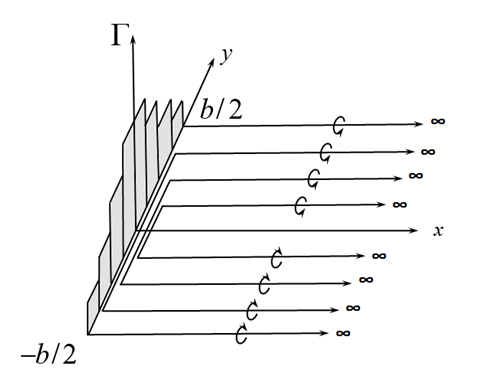
\includegraphics[scale=0.5]{Graphics/horseshoe_vortex.png}
\end{figure}
\Item{Induced Velocity} The downwash at any point $y_0$ is given by
\CenteredBoxed{w(y_0)=-\frac{1}{4\pi}\intlim{-b/2}{b/2}\frac{(d\Gamma/dy)dy}{y_0-y},\ \Gamma=\Gamma(y)}
\Item{Induced Angle of Attack} The induced angle of attack at a location $y_0$ is
$$\alpha_i(y_0)=\arctan\left(\frac{-w(y_0)}{\Vinfty}\right)$$
Substituting the equation for the induced velocity and assuming the magnitude of the induced velocity is much less than that of the free stream velocity (small angle approximation for $\tan$) yields the result
\CenteredBoxed{\alpha_i(y_0) =\frac{1}{4\pi\Vinfty}\intlim{-b/2}{b/2}\frac{(d\Gamma/dy)dy}{y_0-y}}
The induced angle of attack \emph{reduces} the effective angle attack from the geometric angle of attack. It has the effect of tilting the lift vector back (downstream), which reduces lift by $L\cos\alpha_i$ and increases drag by $L\sin\alpha_i$. See illustration below
\begin{figure}[h]
\centering
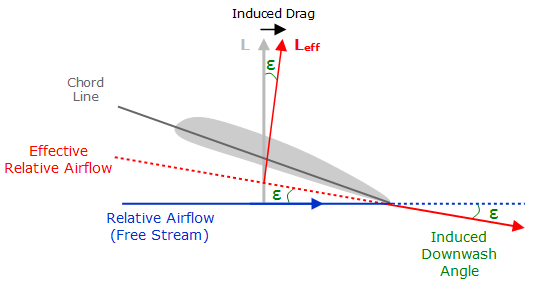
\includegraphics[scale=0.5]{Graphics/induced_diagram.png}
\end{figure}
\Item{Elliptic Lift Distribution} The elliptic lift distribution (not elliptic planform) is the special case of the minimum induced drag and constant downwash (and thus constant induced angle of attack). The distribution is expressed through the elliptic circulation distribution as
$$\Gamma(y)=\Gamma_0\sqrt{1-\left(\frac{2y}{b}\right)^2}$$
through with the lift distribution can be written as
$$L'(y)=\rhoinfty\Vinfty\Gamma_0\sqrt{1-\left(\frac{2y}{b}\right)^2}$$
Find the slope of the circulation distribution as
$$\frac{d\Gamma}{dy}=-\frac{4\Gamma_0}{b^2}\frac{y}{(1-4y^2/b^2)^{1/2}}$$
and integrate such that the induced velocity at a location $\theta_0$ -- parameterization in terms of $\theta$ simplifies integration -- is given by
$$w(\theta_0)=-\frac{\Gamma_0}{2b} = w$$
So the induced angle of attack is given by
$$\alpha_i=-\frac{w}{\Vinfty}=\frac{\Gamma_0}{2b\Vinfty}$$
After integrating the lift distribution and applying the definition of the lift coefficient we arrive at the result
$$ \frac{1}{2}\rhoinfty\Vinfty^2SC_L=L=\rhoinfty\Vinfty\Gamma_0\frac{b}{4}\pi$$
$$\Gamma_0=\frac{2\Vinfty SC_L}{b\pi}$$
\CenteredBoxed{\alpha_i=\frac{C_L}{\pi AR}}
We can then obtain the induced drag from the relation $D_i'=L'\alpha_i$, where the small angle approximation was used, as
\CenteredBoxed{C_{D,i}=\frac{C_L^2}{\pi AR}}
\Item{Oswald Efficiency Factor} The induced drag for a general lift distribution is given by
\CenteredBoxed{C_{D,i}=\frac{C_L^2}{\pi eAR},\ e\leq1}
or, more directly
\CenteredBoxed{C_{D,i}=\frac{C_L^2}{\pi AR}(1+\delta),\ \delta=\sum\limits_2^n n(A_n/A_1)^2\geq0}
The induced drag factor $\delta$ varies with wing geometry (see below)
\begin{figure}[h]
\centering
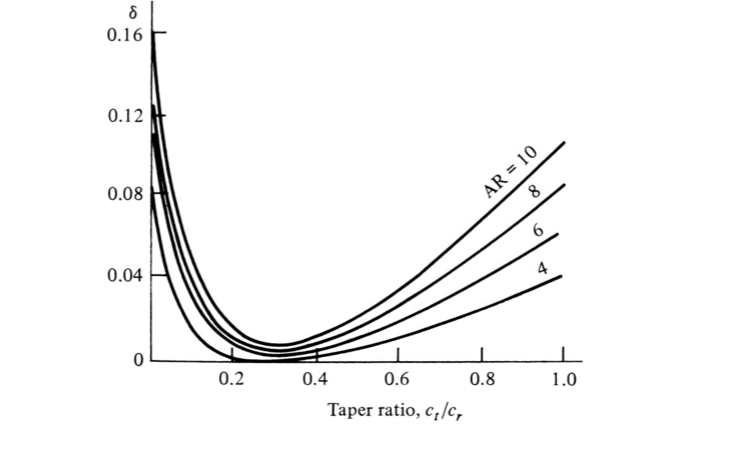
\includegraphics[scale=0.4]{Graphics/delta_vs_lambda.png}
\end{figure}
\Item{Effect of Induced AoA on Lift Curve} The induced angle of attack, being a function of the lift coefficient, has a tendency to reduce the slope of the lift curve. The manner in which it does this is given by
$$\frac{dC_L}{d(\alpha-\alpha_i)}=a_0\implies C_L=a_0(\alpha-\alpha_i)+\mathrm{const}$$
Substituting the result for the induced angle of attack, differentiating and solving for the lift curve slope again, then generalizing the planform gives
$$\frac{dC_L}{d\alpha}=a=\frac{a_0}{1+(a_0/\pi AR)(1+\tau)},\ \tau\in[0.05+0.25]$$
\Item{Vortex Lattice Method} Lifting line theory breaks down for low aspect ratio wings, swept wings, and delta wings. For low AR wings, the tip vortices start to cover a significant portion of the wing. Vortex lattice theory, a panel method, generalizes lifting line theory to be applicable to these cases. The following results are obtained from these modifications (for incompressible flow only):

Low aspect ratio ($AR<4$), straight wing
\CenteredBoxed{a=\frac{a_0}{\sqrt{1+(a_0/\pi AR)^2}+a_0/\pi AR}}

Swept wing ($\Lambda = $  angle of half-chord line with horizontal)
\CenteredBoxed{a=\frac{a_0\cos\Lambda}{\sqrt{1+(a_0\cos\Lambda/\pi AR)^2}+a_0\cos\Lambda/\pi AR}}
\Item{Vortex Lift} Flow will tend to separate along the leading edge of a delta wing (if the LE is sharp) and reattach further down the wing. The high energy vortex has low \emph{static} pressure. This suction effect generates lift at high angles of attack (angles at which conventional wings would stall). A significant portion of the lift is generated near the leading edge of the delta.
\end{itemize}

\subsubsection{Three-Dimensional Aerodynamics -- Drag}
Many drag effects come into play for 3D aerodynamics. What was termed \emph{profile drag} for 2D aerodynamics is referred to in 3D as \emph{parasite drag}. The parasitic drag can be further broken down into skin friction and pressure components. The pressure component is sometimes called \emph{form drag}. In addition to the indcued drag, derived above, there are interference effects between bodies/parts, excresence effects due to rough surfaces or protrusions, and wave effects due to high speed flows.
\begin{itemize}
\Item{Skin Friction} Drag caused by shear stresses along the outer surface of the body. A direct result of viscous flow, which all real flows are. Viscous shear robs the free stream of momentum and thus exerts a force on the body against the direction of relative motion.
\Item{Interference Drag} A type of form drag which is generated by the mixing of fluid flows between components, such as those around the wing and around the fuselage. Other sources of interference drag may include external fuel tanks or weapons, or engine pylon attachments.
\Item{Excresence Drag} A type of form drag which is generated by non-perfectly matched surfaces. Gaps in the outer surface of a body or abrupt changes in shape can cause flow separation, leading to an increase in adverse pressure. Common occurences of excresence drag are windows and control surface hinges.
\Item{Wave Drag} Arises from high speed flows and the shocks associated with them. An aircraft does not necessarily need to be flying supersonic to experience wave drag; the flow may approach sonic speeds as it accelerates over the top of the wing, and the local weak shock can greatly increase the drag coefficient. The exact free stream Mach number where this occurs is called the critical Mach number $M_{cr}$ and is typically around 0.85.
\end{itemize}

Low-speed drag is dominated by induced effects. The high angles of attack necessary for generating sufficient lift at low speeds adds significantly to the drag and the small angle approximation is no longer valid. At higher speeds, the parasitic drag dominates. This particularly relevant for civil transport vehicles, which spend a majority of their time in the relatively high-speed cruise condition. There is more than enough lift available a cruising speeds so the focus is then on minimizing the form drag of the vehicle. Compare and contrast this to the low-speed takeoff and landing segments.\\

High speed drag can be approximated by the Prandtl-Glauert Transformation, which can be approximated as
$$C_D \propto \frac{1}{\sqrt{M_\infty-1}}$$
With $M_\infty>1$ the drag force actually decreases as higher speeds are achieved. This holds true to supersonic flows but not necessarily for the hypersonic regime.

\subsection{Performance}
\subsubsection{Equations of Motion} 
\begin{center}\textbf{\emph{DRAW THE DIAGRAMS}}\end{center}
\CenteredBoxed{m\frac{d\Vinfty}{dt}=T\cos\varepsilon-(D+W\sin\theta)}
\CenteredBoxed{m\frac{\Vinfty^2}{R_1}=(L+T\sin\varepsilon)\cos\phi-W\cos\theta}
\CenteredBoxed{m\frac{(\Vinfty\cos\theta)^2}{R_2}=(L+T\sin\varepsilon)\sin\phi}
\subsubsection{Mattingly's Master Equation}
\CenteredBoxed{\frac{\TSL}{\WTO}=\frac{\beta}{\alpha}\left[\frac{\qinfty S}{\beta\WTO}\left(C_{D,0}+\frac{nk_1\beta}{\qinfty}\left(\frac{\WTO}{S}\right)+\frac{n^2k_2\beta^2}{\qinfty^2}\left(\frac{\WTO}{S}\right)^2+\frac{R}{\qinfty S}\right) + \frac{1}{\Vinfty}\frac{d}{dt}\left(h+\frac{\Vinfty^2}{2g}\right)\right]}

Derivation:
$$P_s = \dot{z}_e=\frac{d}{dt}\left(mgh+\frac{1}{2}m\Vinfty^2\right)$$
$$\frac{P_s}{W}=\frac{d}{dt}\left(h+\frac{\Vinfty^2}{2g}\right)$$
$$\frac{(T-D-R)\Vinfty}{W}=\frac{d}{dt}\left(h+\frac{\Vinfty^2}{2g}\right)$$
$$\frac{T}{W}=\frac{1}{W}\left(D+R\right)+\frac{1}{\Vinfty}\frac{d}{dt}\left(h+\frac{\Vinfty^2}{2g}\right)$$
$$D=\qinfty SC_D=\qinfty S\left(C_{D,0}+k_1C_L+k_2C_l^2\right)$$
$$C_L=\frac{L}{\qinfty S}=\frac{nW}{\qinfty S}$$
$$\frac{T}{W}=\frac{\qinfty S}{W}\left(C_{D,0}+k_1\frac{nW}{\qinfty S}+k_2\left(\frac{nW}{\qinfty S}\right)^2 +\frac{R}{\qinfty S}\right)+\frac{1}{\Vinfty}\frac{d}{dt}\left(h+\frac{\Vinfty^2}{2g}\right)$$
$$W=\beta\WTO,\quad T=\alpha\TSL$$
$$Q.E.D.$$
\subsubsection{Master Equation Responses}
\begin{itemize}
\Item{Terms} Master equation consists of constant, inverse, and linear terms
$$\frac{\TSL}{\WTO}\approx a_0 + a_1\left(\frac{\WTO}{S}\right)^{-1}+a_2\left(\frac{\WTO}{S}\right)$$
\end{itemize}
\subsubsection{Turn Radii}
Turn radius can be calculated from the load factor or vice versa via the equations of motion. Assuming thrust is aligned with the free stream ($\varepsilon=0$) for a steady level turn
\CenteredBoxed{m\frac{\Vinfty^2}{R_2}=nmg\sin\phi\implies R_2=\frac{\Vinfty^2}{ng\sin\phi}}
$$n=\frac{1}{\cos\phi}\implies\frac{1}{n^2}+\sin^2\phi = 1\implies R_2 = \frac{\Vinfty^2}{g\sqrt{n^2-1}}$$
\CenteredBoxed{\omega=\frac{\Vinfty}{R_2} = \frac{g\sqrt{n^2-1}}{\Vinfty}}
$$T=D=\qinfty S\left[C_{D,0}+K\left(\frac{nW}{\qinfty S}\right)^2\right]$$
\CenteredBoxed{n=\left[\frac{\qinfty}{K(W/S)}\left(\frac{T}{W}-\frac{\qinfty C_{D,0}}{W/S}\right)\right]^{1/2}=\left[\frac{\qinfty}{K(W/S)}\frac{P_s}{W}\right]^{1/2}}

\subsubsection{Range}
\textbf{Thrust-Rated Aircraft}
\CenteredBoxed{R=\left(\frac{L}{D}\right)\left(\frac{\Vinfty}{TSFC}\right)\ln\frac{W_i}{W_f}}
Maximum Range: Assume $\Vinfty$ varies such that $L=W$ with constant $C_L$
$$\Vinfty=\sqrt{\frac{W}{\qinfty SC_L}},\ L=\qinfty SC_L,\ D=\qinfty SC_D$$
\CenteredBoxed{R\propto\frac{C_L^{1/2}}{C_D}}
$$\left(\frac{C_L^{1/2}}{C_D}\right)_{max}\implies\frac{d}{dC_L}\frac{C_L^{1/2}}{C_D}=0$$
$$\frac{d}{dC_L}\frac{C_L^{1/2}}{C_D}=0\implies\frac{1}{2}C_L^{-1/2}(C_{D,0}+KC_L^2)-2C_L^{1/2}(KC_L)=0$$
$$C_L=\sqrt{\frac{C_{D,0}}{3K}}\implies C_D=\frac{4}{3}C_{D,0}$$
\CenteredBoxed{\left(\frac{C_L^{1/2}}{C_D}\right)_{max}=\frac{3}{4}\left(\frac{1}{3KC_{D,0}^3}\right)^{1/4}}

\textbf{Power-Rated Aircraft}
\CenteredBoxed{R=\left(\frac{L}{D}\right)\left(\frac{\eta}{c}\right)\ln\frac{W_i}{W_f}}
Maximum Range:
\CenteredBoxed{R\propto\frac{C_L}{C_D}}
$$\left(\frac{C_L}{C_D}\right)_{max}\implies\frac{d}{dC_L}\frac{C_L}{C_D}=0$$
$$\frac{d}{dC_L}\frac{C_L}{C_D}=0\implies(C_{D,0}+KC_L^2)-2C_L(KC_L)=0$$
$$C_L=\sqrt{\frac{C_{D,0}}{K}}\implies C_D=2C_{D,0}$$
\CenteredBoxed{\left(\frac{C_L}{C_D}\right)_{max}=\sqrt{\frac{1}{4KC_{D,0}}}}

\subsubsection{Endurance}
\textbf{Thrust-Rated Aircraft}
\CenteredBoxed{E=\left(\frac{L}{D}\right)\left(\frac{1}{TSFC}\right)\ln\frac{W_i}{W_f}}
Maximum Endurance:
\CenteredBoxed{E\propto\frac{C_L}{C_D}}
\CenteredBoxed{\left(\frac{C_L}{C_D}\right)_{max}=\sqrt{\frac{1}{4KC_{D,0}}}}

\textbf{Power-Rated Aircraft}
\CenteredBoxed{E=\left(\frac{L}{D}\right)\left(\frac{\eta}{c\Vinfty}\right)\ln\frac{W_i}{W_f}}
Maximum Endurance: Assume $\Vinfty$ varies such that $L=W$ with constant $C_L$
$$\Vinfty=\sqrt{\frac{W}{\qinfty SC_L}},\ L=\qinfty SC_L,\ D=\qinfty SC_D$$
\CenteredBoxed{E\propto\frac{C_L^{3/2}}{C_D}}
$$\left(\frac{C_L^{3/2}}{C_D}\right)_{max}\implies\frac{d}{dC_L}\frac{C_L^{3/2}}{C_D}=0$$
$$\frac{d}{dC_L}\frac{C_L^{3/2}}{C_D}=0\implies\frac{3}{2}C_L^{1/2}(C_{D,0}+KC_L^2)-2C_L^{3/2}(KC_L)=0$$
$$C_L=\sqrt{\frac{3C_{D,0}}{K}}\implies C_D=4C_{D,0}$$
\CenteredBoxed{\left(\frac{C_L^{3/2}}{C_D}\right)_{max}=\frac{1}{4}\left(\frac{3}{KC_{D,0}^3}\right)^{3/4}}

\Header{Wind Effects}\\

For the \emph{same airspeed}, headwind reduces ground speed while tailwind increases ground speed. Mark off the airspeed corresponding to zero ground speed on the $D-V$ plot and draw tangents.\\

\subsubsection{Rate of Climb}
Unaccelerated, climbing flight
$$T-D-W\sin\theta=m\frac{d\Vinfty}{dt}=0$$
$$L-W\cos\theta=m\Vinfty\frac{d\theta}{dt}=0$$
\CenteredBoxed{\frac{dh}{dt}=\Vinfty\sin\theta=\frac{T-D}{W}}

The climb angle $\theta$ is found as
$$\theta=\arcsin\left(\frac{T-D}{W}\right)$$
For turbine-driven aircraft, thrust is (mostly) independent of airspeed. Thus the maximum climb angle occurs at the minimum drag condition. The maximum rate of climb, however, occurs at the minimum required power condition (minimum $D\Vinfty$).

\subsubsection{Power Required}
\CenteredBoxed{P_{req}=D\Vinfty=\frac{1}{2}\rhoinfty\Vinfty^3SC_{D,0}+\frac{2KW^2}{\rhoinfty\Vinfty S}}
Graphically, minimum $\frac{P_{req}}{\Vinfty}$ corresponds with minimum $D$ condition.
\subsubsection{Gliding Flight}
Assume steady, gliding flight (unpowered). Then, for a glide angle $\theta$
$$L=W\cos\theta$$
$$D=W\sin\theta$$
\CenteredBoxed{\left(\frac{L}{D}\right)^{-1}=\tan\theta}
Glide range can be calculated assuming a constant glide angle
$$R=\frac{\Delta h}{\tan\theta}=\frac{L}{D}\Delta h$$
Thus maximum range corresponds to the maximum $L/D$ and, consequently, the minimum glide angle. The minimum sink rate, however, does not correspond to the minimum range. The minimum sink rate is found by
$$\dot{h}=-\Vinfty\sin\theta,\ \sin\theta=\frac{D}{W}=\frac{D}{L}$$
where the last equality was made with the small angle approximation for the glide angle. Then the minimum sink rate corresponds to the minimum power condition
\CenteredBoxed{\dot{h}_{min}\propto\frac{C_D}{C_L^{3/2}}}
this should make sense as the sink rate can be equated to the loss of energy height at constant velocity (constant specific kinetic energy), showing immediately that the minimum rate of power loss corresponds to the minimum sink rate.

\subsection{Propulsion}
\subsubsection{Types of Engines}
\begin{itemize}
\Item{Propeller/Reciprocating Engine} High efficiency, low thrust
\Item{Turbojet} Moderate efficiency, higher thrust
\Item{Rocket} Horrible efficiency, maximum thrust
\end{itemize}
\subsubsection{Thrust and Efficiency}
Thrust is produced by ejecting momentum opposite the direction of desired motion (Newton's $\nth{2}$ law). In the case of engines, the thrust produced is given by
\CenteredBoxed{T = (\dot{m}_{air}+\dot{m}_{fuel})V_j - \dot{m}_{air}\Vinfty}
Assuming the mass flow rate of fuel is significantly less than that of air, this equation reduces to
\CenteredBoxed{T = \dot{m}_{air}(V_j-\Vinfty)}
The power output by the engine is given by
$$P_{out} = T\Vinfty$$
while the gain in kinetic energy of the initially stationary fluid through which the engine passes is given by
$$P_{k} = \frac{1}{2}\dot{m}(V_j-\Vinfty)^2$$
This gain in kinetic energy is wasted (more appropriately ``unused'') by the engine as it does not contribute to the propulsion of the system. Thus the efficiency can be found by dividing the useful power output but the total power produced
$$\eta_p = \frac{T\Vinfty}{T\Vinfty+\frac{1}{2}\dot{m}(V_j-\Vinfty)^2}$$
Substituting the above relations and simplifying yields the following, where $V_j\geq\Vinfty$,
\CenteredBoxed{\eta_p=\frac{2}{1+\frac{V_j}{\Vinfty}}}

Clearly, maximum efficiency is obtained when $V_j=\Vinfty$. At this condition, however, there is not net thrust generated (i.e. zero propulsive \emph{efficacy}). This formulation also reveals the underlying physics of the previous statements about the various types of engines. Propellers add very little kinetic energy to the flow and thus have high efficiency at the expense of not generating a whole lot of thrust. Turbojets, on the other hand, significantly increase the velocity of the jet above that of the free stream, generating lots of thrust in the process but at the expense of low efficiency. Rockets take jet velocity to the extreme.

\begin{itemize}
\Item{Full Thrust Equation} The true equation for thrust using control volume analysis and Newton's Second Law is
\CenteredBoxed{T=(\dot{m}_{air}+\dot{m}_{fuel})V_j-\dot{m}_{air}\Vinfty+(p_e-p_\infty)A_e}
where $p_e$ is the pressure at the exit, $p_\infty$ is the atmospheric pressure, and $A_e$ is the area of the exit. The pressure term is usually small compared to the momentum term and thus can be neglected. Thrust is sensitive to altitude, which hides in the mass flow rate term through the density. As density is proportional to pressure and pressure decreases with altitude, thrust decreases with altitude. Similarly, thrust tends to increase with velocity, though the relationship is more complicated ($V_j\Vinfty-\Vinfty^2$).
\Item{Thrust Specific Fuel Consumption} Defined as the weight of fuel consumed per unit of thrust generated per unit time
\CenteredBoxed{TSFC=\frac{\dot{W}_{fuel}}{T}\equiv\frac{lb}{lb\cdot hr},\quad c_t=\frac{N}{N\cdot s}}
\end{itemize}

\Header{Turbojets}\\
\begin{itemize}
\Item{TSFC Variation}
	\begin{itemize}
	\Item{Typical Value} A safe estimate of sea-level static TSFC is 1 pound per horsepower per hour
	\Item{With Velocity} TSFC increases with Mach number, and thus with velocity at constant altitude, for subsonic speeds. TSFC is relatively insensitive to supersonic Mach number.
	\Item{With Altitude} TSFC is relatively insensitive to altitude. There is a small effect but it can be neglected for preliminary analyses
	\end{itemize}
\Item{Turbojet Anatomy}
	\begin{itemize}
	\Item{Diffuser} Slow incoming air, increase pressure and temperature
	\Item{Compressor} Do work on flow, greatly increase pressure and temperature
	\Item{Combustor} Add fuel and burn at (essentially) constant pressure
	\Item{Turbine} Extract work (pass to compressor)
	\Item{Nozzle} Accelerate gas and exhaust it at $V_j$
	\end{itemize}
\Item{The (Ideal) Brayton Cycle}\\
\begin{minipage}{0.48\textwidth}
	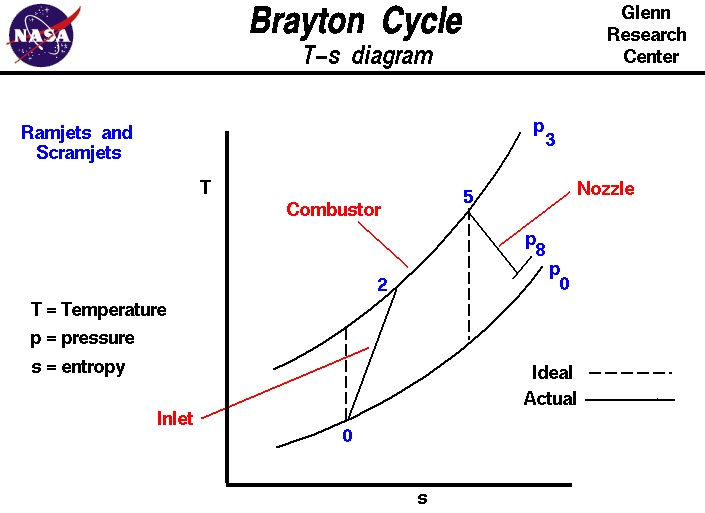
\includegraphics[width=\textwidth]{Graphics/brayton.png}
\end{minipage}
\begin{minipage}{0.48\textwidth}
	\begin{enumerate}
	\item Adiabatic (isentropic) compression
	\item Isobaric heat addition
	\item Adiabatic (isentropic) expansion
	\item Isobaric heat removal
	\end{enumerate}
\end{minipage}
\vspace{1cm}
\Item{Property Profiles}\\
\begin{minipage}{0.48\textwidth}
	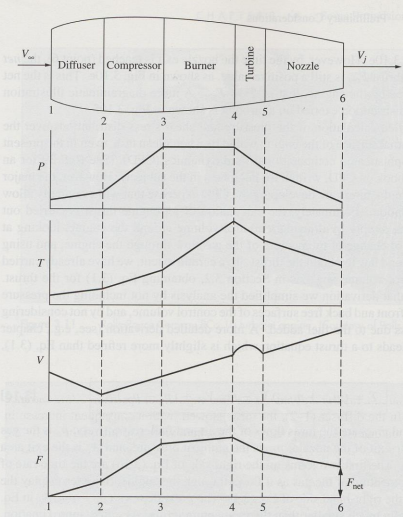
\includegraphics[height = 3in]{Graphics/engine_profiles.png}
\end{minipage}
\begin{minipage}{0.48\textwidth}
	\begin{itemize}
	\item Pressure increases inside the diffuser and compressor, is level through the combustor, then drops through the turbine and nozzle
	\item Temperature increases through the diffuser, compressor, and combustor, then drops through the nozzle and turbine
	\item Velocity decreases in the diffuser, then increases through the compressor and combustor, bumps up then drops through the turbine, and finally increases through the nozzle
	\item A small amount of thrust is generated by the diffuser while the bulk of the thrust is generated by the compressor. The combustor contributes a small amount while the turbine and nozzle generate forces in the drag direction
	\end{itemize}
\end{minipage}
\end{itemize}
\vspace{1cm}

\Header{Turbofans}\\
\begin{itemize}
\Item{Turbofan Terminology}
	\begin{itemize}
	\Item{Bypass Ratio} The ratio of cold air (air around core) to hot air (air through core)
	\Item{Fan Pressure Ratio} Ratio of stagnation pressure before and after the fan
	\Item{Pressure Recovery} Percent of pressure which is retained for useful work. Inlet pressure recovery typically around 90\% while burner pressure recovery is closer to 95\%, though the pressure in the burner is much higher so the losses are greater in magnitude
	\end{itemize}
\Item{Variations for High BPR Turbofans}
	\begin{itemize}
	\Item{Typical Value} About 0.6 pounds per horsepower per hour (almost half that of turbojets)
	\Item{With Velocity} Thrust decreases strongly with velocity, though it is about constant for cruise conditions. TSFC increases with velocity
	\Item{With Altitude} Thrust decreases with altitude for the same reason as turbojets (lower density). TSFC is approximately constant with altitude
	\end{itemize}
\Item{Variations for Low BPR Turbofans}
	\begin{itemize}
	\Item{Typical Value} Closely resembles turbojets, so expect 0.8-0.9 pounds per horsepower per hour
	\Item{With Velocity} Both thrust and TSFC increase with speed
	\Item{With Altitude} Thrust decreases, TSFC approximately constant
	\end{itemize}
\end{itemize}

\Header{Turboprops}\\

Turbine-driven propeller generates more thrust than a reciprocating engine/propeller combination, though less than a turbofan or turbojet. Consumes more fuel than reciprocating engine but less than turbofan or turbojet. Limited to speeds less than critical Mach number for propeller tips.

Turboprops are typically power rated rather than thrust rated. The power output is given by
\CenteredBoxed{P_A=\eta_{pr}P_S+T_j\Vinfty}
where $\eta_{pr}$ is the propeller efficiency, $P_S$ is the shaft power delivered by the engine, and $T_j$ is the thrust provided by the jet. The effective shaft power can be found by dividing by the propeller efficiency
$$P_{es}=P_S+\frac{1}{\eta_{pr}}T_j\Vinfty$$

Specific fuel consumption is based on thrust because basing it on power could lead to confusion over which power term is being referred to. Thus TSFC for turboprops is
$$c_t=\frac{\dot{W}_{fuel}}{T}$$
and a typical static installed thrust conversion is 2.5 pounds per shaft horsepower. TSFC is roughly constant with both velocity and altitude.

Power available is roughly constant with free stream Mach number due to the combined effect of increasing velocity with decreasing thrust (recall $P_A=T_A\Vinfty$). Power available decreases with altitude by a power law
$$P_A=P_{A,0}\left(\frac{\rho}{\rho_0}\right)^n$$
with $n$ depending on the engine (typically around 0.7).\\

\Header{Specific Fuel Consumptions}\\

Sometimes it is useful to be able to convert specific fuel consumptions between power rated and thrust rated aircraft. This can be done as follows and is useful for quickly formulating the range equations for either type of aircraft
$$c_t = \frac{\dot{W}_{fuel}}{T},\ c = \frac{\dot{W}_{fuel}}{P}$$
$$c_t = \frac{cP}{T},\ P = \frac{1}{\eta_{pr}}T\Vinfty$$
$$c_t = \frac{c\Vinfty}{\eta_{pr}}$$

\subsubsection{Alternative Fuels}
Renewable resource for meeting demand. Currently quite expensive and not exactly drop-in compatible, but working towards it.
\subsubsection{Electronic Propulsion}
Vehicle does not shed weight throughout the mission so range and endurance take a hit. Also have to worry about energy density, recharge time, etc.

\subsection{Structures}
\subsubsection{Brittle vs Ductile Materials}
Brittles have high Youngs moduli (relatively) but break abruptly. Ductile materials yield at a certain strain and then go plastic, reaching an ultimate strength before failing.
\subsubsection{Failure and Safety}
Common failure modes include buckling (for thin walled structures) and yield. Factors of safety are applied to the yield stresses to account for manufacturing defects, environmental conditions, inherent variability, and other sources of uncertainty in the applications of materials. A typical safety factors is in the range of 1.5 to 3. There may be a different factor of safety for each expected failure more.
$$\sigma_{des} = \frac{\sigma_{fail}}{S_F}$$
The margin of safety is defined as the ratio of the failure load to the design load, less one
$$\textrm{Margin of Safety} = \frac{\sigma_{fail}}{\sigma_{des}}-1 = S_F-1$$
\subsubsection{Aircraft Loads}
\begin{minipage}{0.63\textwidth}
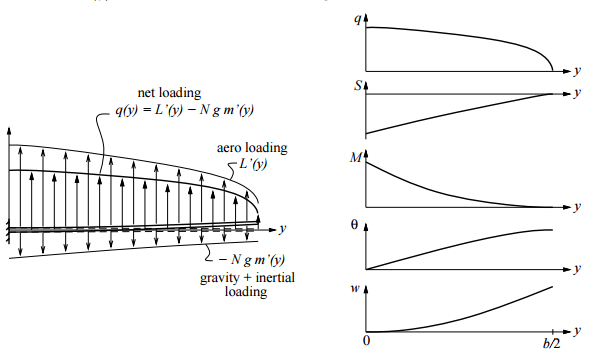
\includegraphics[width=\textwidth]{Graphics/aircraft_loads.png}
\end{minipage}
\begin{minipage}{0.35\textwidth}
$$q(y)=L'(y)-m'(y)$$
$$V(y) = V_0 + \intlim{0}{b/2}q(y)dy$$
$$V(b/2) = 0$$
$$M(y) = M_0 + \intlim{0}{b/2}V(y)dy$$
$$M(b/2) = 0 $$
\end{minipage}

Useful note from MIT document: It can be useful to assume the net distributed load is proportional to the chord distribution with the proportionality constant chosen such that the integrated loads are equal
$$q(y)=Kc(y)$$
$$\intlim{-b/2}{b/2}Kc(y)dy = \intlim{-b/2}{b/2}(L'(y)-m'(y))dy$$
$$KS_W = L-m_{wing}$$
$$K = \frac{L-m_{wing}}{S_W} \approx \frac{m_{fuselage}}{S_W}$$
\subsubsection{V-n Diagram}
The $V$-$n$ diagram shows the relationship between the load factor and speed of an aircraft. It shows the operational envelope -- the values of $V$ and $n$ which are simultaneously feasible. The common choice for $V$ is the equivalent airspeed, which is selected to make the $V$-$n$ diagram altitude-independent. The equivalent airspeed is defined as the airspeed at sea level for which the same lift force is generated (and thus the load factor is the same).
$$V_{EAS} = V(\rho_0)\big|_{L_0=L}$$
$$V = \sqrt{\frac{2L}{\rho SC_L}}$$
$$V_{EAS} = \sqrt{\frac{\rho}{\rho_0}}V = \sqrt{\frac{2nW}{\rho_0SC_L}}$$

\Header{V-n Diagram Constraints}
\begin{itemize}
\Item{Basic Lift Generation} The equation for lift relates the load factor to the square of velocity which, for a fixed vehicle, is scaled by the lift coefficient. Thus the proportionality $n\propto V_{EAS}$ gives two (parabolic) lines which constraint the diagram, typically from the left and above.
\Item{Stall} A load factor of 1 is required for steady level flight, so there is typically a side constraint at the equivalent airspeed where the positive load factor is 1. There may also be one for the $n=-1$ case, for which the equivalent airspeed is typically higher (because $|C_{L,min}|<|C_{L<max}|$).
\Item{Limit Load Factor} These are the actual loads expected in service. These loads must be sustainable without detrimental, permanent damage to the vehicle structure. Deformation may not interfere with safe operation for loads up to the limit loads. Typical values for commercial vehicles are $\pm3$, while those for fighter aircraft are higher. Constrains design space from above and below.
\Item{Ultimate Loads} These the loads which the structure must be able to support for three seconds without global failure (local failure like buckling is okay). The values are those for the limit loads multiplied by a factor of safety, which is typically around 1.5. Extended constraints from above and below.
\Item{Dive Speed} The design dive speed. Vehicle must not experience flutter, control reversal, or divergence up to 1.2$V_D$. Constrains design space from the right.
\Item{Gust Loads} Gusts will increase the load factor on the vehicle. By assuming the gust velocity is much less than the vehicle airspeed we can employ the small angle approximation and come up with a change in load factor which is linearly proportional to the equivalent airspeed for a given gust speed. This is derived from analyzing the gust as an instantaneous change in angle of attack. There are two important gust speeds: one which must be sustained up to the cruise velocity, and one which must be sustained up to the design dive speed.
\end{itemize}

The vehicle must be able to operate safely within all of the above constraints, and testing is often performed at the intersections of the lines (red corners, below) which are considered the critical conditions.
\begin{figure}[h]
\centering
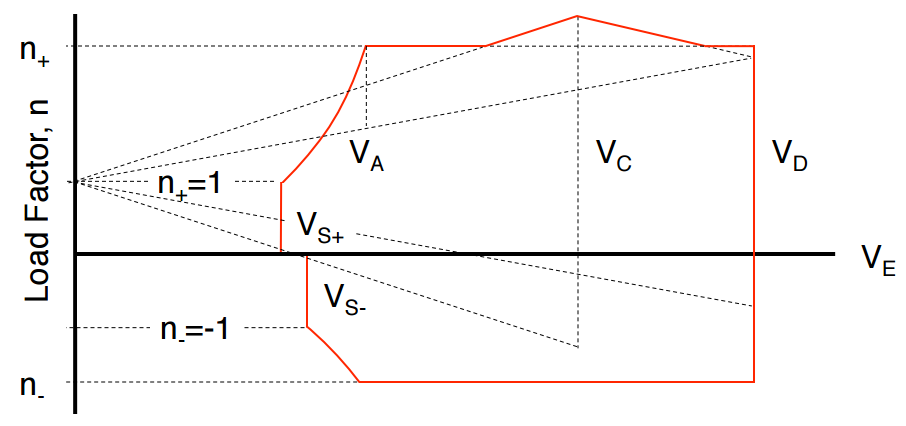
\includegraphics[width=\textwidth]{Graphics/V-n.PNG}
\end{figure}

\subsection{Stability and Control}
\subsubsection{Types of Stability}
Definition: Stability is the tendency of a system to maintain or deviate from an initial, established condition.
Definition: Control is the ability of a system to move between states/conditions at will
\begin{itemize}
\Item{Stable} A system is stable if any small perturbations from an equilibrium state die out with time, restoring the system to the equilibrium state
\Item{Unstable} A system is unstable if any small perturbations from an equilibrium state oscillates around or diverges from the equilibrium state
\Item{Neutral} A system is neutrally stable if disturbances neither grow nor die out with time (e.g. perfect harmonic motion)
\Item{Static Stability} A system is statically stable if its initial response to a disturbance pushes it back towards its initial state (over damped stability)
\Item{Dynamic Stability} A system is dynamically stable if disturbances oscillate about the equilibrium state but decay in magnitude with time (under damped stability). Most dynamically stable systems are also statically stable (i.e. the initial response is back towards equilibrium, it just overshoots and comes back repeatedly)
\end{itemize}

A ball in a valley is stable, a ball on top of a hill is unstable. A frictionless pendulum is statically stable and dynamically neutral; a pendulum with friction is statically and dynamically stable; an inverted pendulum is statically unstable (can't even talk about dynamic properties for this case).
\subsubsection{Stability Derivatives}
Stability is often described in terms of coefficients, much like lift, drag, and moment. The coefficients in this case are the roll, pitch, and yaw moments
$$\textrm{Pitch: }C_m = \frac{M}{qSb}$$
$$\textrm{Yaw: }C_n = \frac{N}{qS\bar{c}}$$
$$\textrm{Roll: }C_l = \frac{L}{qSb}$$
Note that wing span is used as the reference length for the roll and yaw moments while mean aerodynamic chord is used for the pitching moment. The stability derivatives are taken with respect to the relevant angles, and their sign is important in talking about vehicle stability.

\subsubsection{General Stability}
A vehicle will be stable if it is able to damp out disturbances and deviations from steady level flight. That is, a change in angle of attack $\alpha$, side slip angle $\beta$, or roll angle $\phi$ should decay with time, per our definition of stability. This requires the vehicle must provide restoring moments when exposed to the aforementioned deviations. Since the moments depend on the angles themselves, we can express this via partial derivatives
$$\Partial{C_m}{\alpha}<0$$
$$\Partial{C_n}{\beta}>0$$
$$\Partial{C_l}{\phi}<0$$

\subsubsection{Static Margin}
The static margin is the distance between the center of gravity of the aircraft and its neutral point (the point where neutral stability is achieved), typically expressed as a percentage of the mean aerodynamic chord. Mathematically, the static margin represents the (negative of the) derivative of the pitching moment coefficient with respect to the lift coefficient. 
\CenteredBoxed{\Partial{C_M}{C_L}=-\left(\frac{x_{NP}-x_{cg}}{MAC}\right) = -K}

This is also known as pitch stiffness. Note that if $K$ is positive then the neutral point is \emph{aft} of the center of gravity, and the pitching moment will \emph{decrease} as the lift coefficient (i.e. the angle of attack) increases, creating a stable negative feedback loop. If $K$ were negative then increasing the angle of attack would increase the pitching moment, further increasing the angle of attack. This is characteristic of an unstable positive feedback loop and is generally undesirable.

\subsection{Other Considerations}
\subsubsection{Subsystem Integration}
Most subsystems take power off from the engine, and there can be significant transmission and/or conversion losses for the different forms of power/energy (electric, mechanical, pneumatic, hydraulic). The environmental control unit (ECU) is a big one, along with the flight controls. Taking power off of the engine reduces fuel efficiency and thus harms overall performance, so care needs to be taken when designing and integrating subsystems (and the engine, too).

\subsubsection{Aircraft Economics}
Life cycle cost analysis can be used to determine the economic viability of an aircraft. The life cycle includes all four design phases, manufacturing, operation, maintenance, logistics, and disposal. These costs are borne by a variety of stakeholders and the decades-long life means inflation and interest come into play.

%%%%%%%%%%%%%%%%%%%%%%%%%%%%%%%%%%%%%%%%%%%%%%%%%%%%%%

\section{Optimization}
\subsection{Standard Form of an Optimization Problem}
$$\mathrm{Minimize}\ f(\boldx)$$
$$\mathrm{w.r.t.}\ \boldx=[x_1,x_2,\dots,x_n]$$
$$s.t.\ g_j(\boldx)\leq0\ \forall j\in\mathbb{J},\ h_k(\boldx)=0\ \forall k\in\mathbb{K}$$
$$\boldx_l\leq\boldx\leq\boldx_u$$

For maximization, simply negate the objective function $f'(\boldx)=-f(\boldx)$

\subsection{Conditions for Optimality}
\subsubsection{First Order Necessary}
\begin{itemize}
\Item{Karush-Kuhn-Tucker Conditions} If a point $\xstar$ is optimal then the following hold
	\begin{enumerate}
	\item $\xstar$ is feasible
	\item $\lambda_jg_j(\xstar)=0\ \forall j\in\mathbb{J}$ (complimentary slackness)
	\item $\nabla\mathcal{L}(\xstar,\lambda)=\nabla f(\xstar)+\sumlim{j=1}{m}\lambda_j\nabla g_j(\xstar)+\sumlim{k=m+1}{\mathcal{N}}\lambda_kh_{(k-m)}(\xstar)=0,\ \lambda_i\geq0\ \forall i\in[1,\mathcal{N}]$
	\end{enumerate}
\item There are no first order \emph{sufficient} conditions for optimality. That is, there are no conditions such that a point $\xstar$ which satisfies those conditions is guaranteed to be an optimum.
\Item{Strong vs Weak Optima} An optimum $\xstar$ is a strong optimum if
\CenteredBoxed{\xstar<\boldx\ \forall \boldx\in[\xstar-\varepsilon,\xstar+\varepsilon]}
An optimum $\xstar$ is a weak optimum if
\CenteredBoxed{\xstar\leq \boldx\ \forall \boldx\in[\xstar-\varepsilon,\xstar+\varepsilon]}
\end{itemize}
\subsubsection{Second Order Necessary and Sufficient}
\begin{itemize}
\Item{The Hessian} Defined as
\[H\left(f(x_1,x_2,\dots,x_n)\right) =  \begin{bmatrix}
\PPartial{f}{x_1} & \PPPartial{f}{x_1}{x_2} & \dots & \PPPartial{f}{x_1}{x_n}\\
\PPPartial{f}{x_2}{x_1} & \PPartial{f}{x_2} & \dots & \PPPartial{f}{x_2}{x_n}\\
\vdots & \vdots & \ddots & \vdots\\
\PPPartial{f}{x_n}{x_1} & \PPPartial{f}{x_n}{x_2} & \dots & \PPartial{f}{x_n}
\end{bmatrix}\]
\Item{Necessary Conditions for Optimality} Same as first order necessary
\Item{Sufficient Conditions for Optimality} A point $\xstar$ is a global optimum if the Hessian of $f$ at $\xstar$ is positive definite (all eigenvalues are positive). A point $\xstar$ is a local optimum if the Hessian of $f$ at $\xstar$ is positive semidefinite (all eigenvalues are non-negative). These assume the goal of optimization is minimization.
\Item{Eigenvalues of the Hessian} The eigenvalues of the Hessian $\lambda_e$ are found by taking the determinant of $\Hessian(f)-\lambda_e\mathbb{I}$ and solving the resulting polynomial for $\lambda_e$

\end{itemize}

\subsection{Line Searches}
\subsubsection{Golden Section Method}
\begin{itemize}
\Item{Purpose} The Golden Section Method (GSM) is a line search technique which iteratively reduces the searchable space which brackets a minimum. The same proportional of the searchable space is thrown out with each iteration until convergence is achieved. W.L.O.G. assume $f$ is a function of only one variable.
\Item{Bracketing a Minimum} Three function values $f_1$, $f_2$, and $f_3$, evaluated at $x_1$, $x_2$, and $x_3$, respectively, with $x_1<x_2<x_3$, bracket a minimum if $f_2<f_1$ \emph{and} $f_2<f_3$. There are no guarantees about the strength of the bracketed minimum.
\Item{Steps in GSM}
	\begin{enumerate}
	\item Bracket a minimum
	\item Evaluate four points within the bracketed space: the two end points, $x_l$ and $x_u$, and two in between, $x_1$ and $x_2$
	\item Determine which endpoint to toss based on bracketing criteria. That is, determine if $\{x_l,x_1,x_2\}$ brackets the min or if $\{x_1,x_2,x_u\}$ brackets the min. Toss the end point which is not in the set which brackets the min
	\item Reassign the endpoints and generate a fourth point inside the bracket
	\item Repeat steps 3 and 4 until the desired tolerance is reached
	\end{enumerate}
\Item{Picking the New Point} The new point in the bracketed space is determined by the Golden Ratio (hence the name). This is motivated by the desire to reduce the bracketed space by the same proportion at each iteration (this is desirable because it ensures a consistent spacing of the points). The proportion is derived, from the below figure, as follows:
\begin{figure}[h]\centering
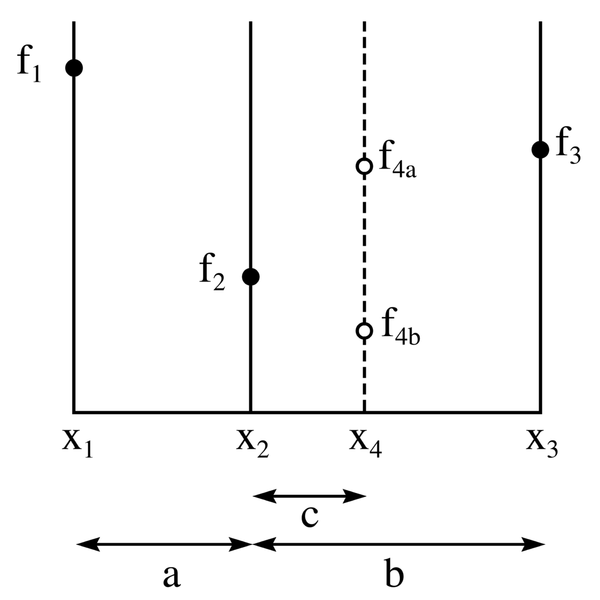
\includegraphics[scale=0.2]{Graphics/GSM.png}
\end{figure}
$$\textrm{We want } \frac{c}{a}=\frac{a}{b}\textrm{ (i.e. same proportion eliminated each time), and } c=b-a$$
$$\frac{b-a}{a}=\frac{a}{b}\to\frac{b}{a}-1=\frac{a}{b}$$
$$\frac{b}{a}\left(\frac{b}{a}-1=\frac{a}{b}\right)\to\left(\frac{b}{a}\right)^2-\frac{b}{a}-1=0$$
$$\frac{b}{a}=\frac{1\pm\sqrt{1-4(1)(-1)}}{2}=\frac{1\pm\sqrt{5}}{2}$$
\CenteredBoxed{\frac{b}{a}=1.618}
\indent The negative root was tossed for obvious reasons
\end{itemize}
\subsubsection{Direction Finding}
\subsubsection{Finding $\alpha^*$}
The methods here are of concern when a GSM is not being used. They are relevant for methods where the algorithm seeks to advance a reasonable distance along a direction, and determining what that distance should be.
\begin{itemize}
\Item{The Wolfe Conditions} The Wolfe conditions are two conditions which can be used to determine the step size along a given direction. They come in strong and weak forms. The weak form is to find $\alpha$ such that the following hold
	\begin{enumerate}
	\item Armijo: $\boxed{f(\boldx_{k-1}+\alpha\mathbf{s}_k)\leq f(\boldx_{k-1})+c_1\alpha\mathbf{s}_k^T\nabla f(\boldx_{k-1}}$. This rule requires the function to not change too much along the given search direction. The ''too much'' conditional is expressed through the constant $c_1\in[0,1]$ and typically $c_2\approx 10^{-4}$, and the gradient of the function (higher gradients allow for larger step sizes)
	\item Curvature: $\boxed{\mathbf{s}_k^Tf(\boldx_{k-1}+\alpha\mathbf{s}_{k-1})\geq c_2\mathbf{s}_k^T\nabla f(\boldx_{k-1})}$. This condition requires the step size to be large enough that the gradient changes meaningfully. The `'meaningful'' conditional is expressed through the constant $c_2\in[0,1]$ and typically $c_2\approx0.9$. Note that gradients will be negative in the search direction (assuming minimization) so the gradient should become \emph{less negative}
	\end{enumerate}
	
	The strong form is to find $\alpha$ such that the following hold
	\begin{enumerate}
	\item Armijo: $\boxed{f(\boldx_{k-1}+\alpha\mathbf{s}_k)\leq f(\boldx_{k-1})+c_1\alpha\mathbf{s}_k^T\nabla f(\boldx_{k-1}}$. Unchanged from weak conditions
	\item Curvature: $\boxed{|\mathbf{s}_k^Tf(\boldx_{k-1}+\alpha\mathbf{s}_{k-1})|\leq c_2|\mathbf{s}_k^T\nabla f(\boldx_{k-1})|}$. Now we require that the \emph{magnitude} of the gradient decrease by a meaningful amount 
	\end{enumerate}
\end{itemize}

\subsection{Indirect Methods for Constrained Optimization}
Indirect methods provide means to incorporate constraints into the optimization formulation. They work by augmenting the initial objective function such that the new pseudo-objective function can be minimized in an unconstrained way (e.g. line search). They may, however, provide suboptimal or infeasible results if proper care is not taken in their formulation.
\subsubsection{Exterior Penalty Method}
Perhaps the simplest of the indirect methods, the exterior penalty method adds the constraint value to the objective value when the constraint is active. That is, the augmented objective function becomes
\CenteredBoxed{\Phi(\boldx,r_p)=f(\boldx) + r_p\left[ \sumlim{j=1}{l}\max[0,g_j(\boldx)]^2 + \sumlim{k=1}{m}[h_{k}]^2\right]}
where the variable $r_p$ scales the penalty for violating any of the constraints. Typically, $r_p$ will start small and increase as the optimization procedure goes on.

The exterior penalty method has a tendency to allow infeasible designs. The penalty may not be able to overcome the gradient of the objective at the boundary if the gradient is steep enough, and thus may require $r_p\to\infty$, which is impractical. The function also becomes extremely nonlinear at the boundaries which could cause problems for line searches. It is, however, extremely simple to implement.

\subsubsection{Interior Penalty Method}
The interior penalty method only applies to inequality constraints (equality constraints have no interior). The method imposes a penalty for getting close the constraint boundaries, then relaxes those penalties as the procedure advances. This formulation allows the optimizer to approach the optimum from within the feasible space. It may, however, yield suboptimal results if the procedure is terminated early. The augmented objective function becomes
\CenteredBoxed{\Phi(\boldx,r_p,r_p')=f(\boldx) + r_p'\sumlim{j=1}{l}\frac{-1}{g_j(\boldx)} + r_p\sumlim{k=1}{m}[h_{k}]^2}
where $r_p'$ is a new penalty factor which starts very large and decreases (to one) as the optimization procedure advances. An alternative formulation uses the logarithm of the inequality constraints, becoming
\CenteredBoxed{\Phi(\boldx,r_p,r_p')=f(\boldx) + r_p'\sumlim{j=1}{l}-\log[-g_j(\boldx)] + r_p\sumlim{k=1}{m}[h_{k}]^2}

\subsubsection{Extended Interior Penalty Method}
Similar to the standard interior penalty method but with a modification to enable finding truly optimal points. Each inequality constraint is modified such that
\[\tilde{g}_j(\boldx)=\begin{cases}
\frac{-1}{g_j(\boldx)} & g_j(\boldx)\leq\varepsilon\\
-\frac{2\varepsilon-g_j(\boldx)}{\varepsilon^2} & g_j(\boldx)>\varepsilon
\end{cases}\]
with $\varepsilon = -c(r_p')^a$, $-1/3\leq a\leq1/2$ and $c=const.$. This linearizes the constraint near the boundary on the feasible side

\subsubsection{Constraint Scaling}
Constraints can be scaled to the order of the objective function. This is done to aid smoothness of the pseudo-objective, which in turn helps whatever methods are chosen for finding the optimum. Constraints should be scaled according to
$$\bar{g}_j(\boldx)=c_jg_j(\boldx)$$
$$c_j=\frac{|\nabla f(\boldx)|}{|\nabla g_j(\boldx)|}$$
With these scalings, the initial values for the penalty factors $r_p$ and $r_p'$ are one.

\subsubsection{The Augmented Lagrangian}
The Augmented Lagrangian combines Lagrange's method of undetermined coefficients with the exterior penalty method to come up with a new pseudo-objective function. The ALM pseudo-objective is given by
$$\mathbf{A}(\boldx,\lambda,r_p)=\mathcal{L}(\boldx,\lambda) + r_p\left[\sumlim{j=1}{l}g_j(\boldx)^2 + \sumlim{k=1}{m}\left(h_k(\boldx)\right)^2\right]$$
\CenteredBoxed{\mathbf{A}(\boldx,\lambda_p,r_p) = f(\boldx) + \sumlim{j=1}{l}\left[\lambda_j\psi_j(\boldx) + r_p\left[\psi_j(\boldx)\right]^2\right] + \sumlim{k=1}{m}\left[\lambda_{p,k+m}h_k(\boldx) + r_p[h_k(\boldx)]^2\right]}
where
$$\psi_j(\boldx)=\max\left[g_j(\boldx),\frac{-\lambda_{p,j}}{2r_p}\right]$$
The augmented Lagrangian is derived from a comparison of the standard Lagrangian and the exterior penalty methods, as follows.
\begin{itemize}
\item Consider a potential optimal point $\xstar$. At this point, the following must hold
$$\nabla\mathcal{L}(\xstar,\lambda) = \nabla f(\xstar) + \sumlim{\textrm{active}}{}\lambda_j\nabla g_j(\xstar) + \sum\lambda_k\nabla h_k(\xstar) = 0$$
$$\nabla\Phi(\xstar,r_p) = \nabla f(\xstar) + r_p\left[\sumlim{\textrm{active}}{}2g_j(\xstar)\nabla g_j(\xstar) + \sum2h_k(\xstar)\nabla h_k(\xstar)\right] = 0$$
\item Equating these two equations and comparing the coefficients of the derivatives yields
$$2r_pg_j(\xstar)=\lambda_j,\quad 2r_ph_k(\xstar)=\lambda_k$$
which, after rearranging and applying complimentary slackness from the KKT conditions, reveals that we require $r_p\to\infty$
\item We can get around the $r_p\to\infty$ problem by realizing the gradient augmented Lagrangian must go to zero along with that of the true Lagrangian itself. That is,
$$\nabla\mathbf{A}(\xstar,\lambda_p,r_p)=\nabla\mathcal{L}(\xstar,\lambda)=0$$
\item After applying the gradients and simplifying, we arrive at the following
$$\lambda_j=\lambda_{p,j}+2r_p\max\left[g_j,\frac{-\lambda_{p,j}}{2r_p}\right]$$
$$\lambda_k=\lambda_{p,k}+2r_ph_k(\xstar)$$
These formulas can be used to update the Lagrange multiplier estimates at each iteration while maintaining complimentary slackness and being relatively insensitive to choices in $r_p$
\item A note on Lagrange multipliers: They can be roughly interpreted as the cost of having that constraint be there. Consider a function with one constraint evaluated at the optimum point where that constraint is active. Then the following holds
$$\nabla f(\xstar)+\lambda\nabla g(\xstar)=0$$
$$\lambda=\frac{-\nabla f(\xstar)}{\nabla g(\xstar)}$$
Thus $\lambda$ can be interpreted as the ratio of the improvement in $f$ to the degradation of $g$. High Lagrange multipliers imply significant improvement may be made in the objective function by relaxing that constraint, relative to the penalty incurred by that constraint. Complimentary slackness tells us there is no benefit to relaxing an inactive constraint.
\end{itemize}

\subsection{Zeroth Order Methods}
\subsubsection{Compass Search}
From a starting location sample a $\pm1$ unit step in each design variable independently. Move to the point which provides the best improvement over the current point. Repeat at new point (obviously not re-sampling the point you just came from).
\subsubsection{Univariate Search}
Perform the GSM algorithm along each design variable independently and iteratively (i.e. GSM along $x_1$, then $x_2$, and so on to $x_n$, then repeat).
\subsubsection{Powell's Method}
\begin{itemize}
\Item{Overview} Apply conjugacy condition to univariate search algorithm to improve convergence behavior
\Item{Method}
	\begin{enumerate}
	\item Do one pass over the univariate search method (i.e. do GSM in each univariate direction)
	\item Determine the $(n+1)^{th}$ search direction such that is is conjugate to all other directions
	\item Definition of conjugacy: Two vectors $\mathbf{s}_i$ and $\mathbf{s}_j$ are conjugate w.r.t. a matrix $\mathbb{A}$ if
	$$\mathbf{s}_i'\mathbb{A}\mathbf{s}_j=0$$
	in the case of Powell's method $\mathbb{A}=\mathbb{I}$ and $\mathbf{s}_{n+1}=\sumlim{i=1}{n}\alpha_i\mathbf{s}_i$ where $\mathbf{s}_i$ are unit vectors and $\alpha_i$ is the distance between the initial and final points for the $i^{th}$ search direction. The $(n+1)^{th}$ search direction is simply the (normalized) weighted sum of the previous $n$ search directions, with the step size as the weighting criteria
	\end{enumerate}
\Item{Benefits} For a quadratic problem with $n$ variables, convergence will be achieved in at most $n$ cycles
\Item{Drawbacks} Search directions tend to coalesce as the algorithm gets into its later stages (requires resetting search directions to univariates)
\end{itemize}

\subsection{First Order Methods}
First order methods are mostly concerned with determining the search direction from derivative information and performing line searches in those directions.
\subsubsection{Steepest Descent}
\begin{itemize}
\Item{Definition} Steepest descent picks the search direction which provides the most rapid improvement in the objective function. That is, the search direction is found to be
\CenteredBoxed{\mathbf{s}_k=\frac{-\nabla f(\boldx_{k-1})}{\|f(\boldx_{k-1})\|}}
\end{itemize}
\subsubsection{Fletcher-Reeves Conjugate Gradient}
The Fletcher-Reeves method applies conjugacy to the gradient of the objective function at each point, analogous to how Powell's applied conjugacy to directions. The new search direction is found via the update method
\CenteredBoxed{\mathbf{s}_{k+1}=-\nabla f_{k}+\beta_k\mathbf{s}_{k}}
$$\beta_k=\frac{\|\nabla f_{k}\|^2}{\|\nabla f_{k-1}\|^2}$$

Fletcher-Reeves modifies the steepest descent direction with derivative information from previous steps. The first direction will be the steepest descent direction
\subsubsection{Broyden-Fletcher-Goldfarb-Shanno Quasi-Newton Method}
BFGS uses an approximation of the Hessian matrix to find the search direction. The Hessian is approximated by applying a finite difference to gradient information and updating the approximation as the algorithm proceeds. The method finds the search direction as
\CenteredBoxed{\mathbf{s}_{k+1}=-B_k\nabla f(\boldx_k)}
where
\CenteredBoxed{B_{k+1}=B_k+\frac{(\Delta(\nabla f_{k,k-1})-B_k\Delta\boldx_{k,k-1})(\Delta(\nabla f_{k,k-1})-B_k\Delta\boldx_{k,k-1})^T}{(\Delta(\nabla f_{k,k-1})-B_k\Delta\boldx_{k,k-1})^T\Delta\boldx_{k,k-1}}}
and $B_0=\mathbb{I}$ (i.e. first direction is steepest descent)
\subsection{Second Order Methods}
\subsubsection{Newton's Method}
Newton's method finds the next search direction by inclusion of Hessian (second order) information. The search direction is found via
\CenteredBoxed{\mathbf{s}_{k+1}=-\left[H(\boldx_k)\right]^{-1}\nabla f(\boldx_k)}
\begin{itemize}
\Item{Benefits} If the function is quadratic then Newton's method will find the optimum in one step
\Item{Drawbacks} The inverse of the Hessian may not exist (if it is not positive definite) and can be computationally expensive if it is. BFGS is one way to work around this
\end{itemize}

\subsection{Multi-Objective Optimization}
\subsubsection{Domination Criteria and Pareto Optimality}
Optimality is more difficult for multi-objective problems because of the comparability problem. It would be impossible to compare two designs unless we were able to apply a strict preference to the set of objectives. One way around this is Pareto analysis, in which the set of best designs is separated from the rest of the space. The Pareto optimal set consists of all nondominated designs, either strongly or weakly so. A design is said to be strongly nondominated if there exists no other design whose objective values are strictly better than its own. That is, assuming minimization is the objective,
$$\xstar\in\mathbb{P}\iff f(\xstar)<f(\boldx)\ \forall\boldx\in\mathbb{D}\ \&\ \forall f\in\mathbb{F}$$
Weak domination removes the strictness of the inequality
$$\xstar\in\mathbb{P}\iff f(\xstar)\leq f(\boldx)\ \forall\boldx\in\mathbb{D}\ \&\ \forall f\in\mathbb{F}$$

\subsubsection{Finding the Pareto Frontier}
\begin{itemize}
\Item{Weighted Sum Approach} Consolidate the multiple objective functions into a single objective which is a weighted sum of all the objectives. Changing the weighting scheme changes where on the Pareto front the algorithm will converge. Benefits: Easy. Drawbacks: Cannot sample convex spaces
\Item{Epsilon-Constraint Method} The epsilon-constraint method reduces the multi-objective problem to a single objective problem by converting the other objective(s) into constraints. The optimizer will then seek to optimize a the free objective while keeping the other(s) below a given margin. This is best visualized with a two-objective minimization problem
\Item{Normal Boundary Intersection} Designed to evenly sample the Pareto frontier. For a 2D problem this method draws a line between the best points in each objective dimension, then moved in the normal direction to that line (in the improvement direction, of course) until the optima along that line are found. This can be thought of as minimizing $f_1$ subject to $f_2=\alpha+\beta f_1$
\end{itemize}

\subsection{Metaheuristic Methods}
\subsubsection{Particle Swarm}
Based loosely on swarm animal/insect behaviors, each design point moves according to some rules so as to improve its own objective value. Particles may interact with neighbors or entire swarm. Velocity update may include inertia (history), local best, global best, pushoff factors, or other terms.
\subsubsection{Simulated Annealing}
Based on the idea of a cooling piece of metal and the minimization of energy within the crystalline structure. A cooling schedule governs the likelihood of accepting a new point with a worse objective value, while points with better objective values are always taken. Probability of accepting a new point $\xstar$ from a starting point $\boldx$ given by decaying exponential
$$P(\boldx,\textrm{accept }\xstar) = \min\left[e^{-\Delta E/kT_i},1\right]$$
$$\Delta E = f(\xstar)-f(\boldx)$$
$$T_i=\gamma T_{i-1},\ \gamma<1$$
Clearly if $\Delta E$ is negative ($f(\boldx)>f(\xstar)$) then the probability is greater than one. The decrease of $T$ with each iteration makes the exponent more negative for the same $\Delta E$, meaning worse candidate points are less likely to be accepted.
\subsubsection{Genetic Algorithm}
The genetic algorithm takes inspiration from biology. Design variable vectors are converted to chromosomes with each gene representing a single design variable. The objective function values determine the fitness of an individual. Crossover and mutation provide the means for exploitation and exploration, respectively. The NSGA-II uses Pareto frontier information to select the best candidates at each generation, which then carry over to the next generation.

GAs require the design variables to be discretized. This can give rise to issues with extremely long chromosomes resulting from very fine resolutions or missing large parts of the design space because the discretization is too coarse. The number of bits required for a given range and resolution on a design variable is given by
$$N\geq\log_2\left(\frac{Range}{Resolution}+1\right)$$

Gray coding can be used to avoid the Hamming cliff problem. The Hamming cliff problem arises from binary representations because the number of bits which must flip to increment a variable by one unit may be extremely large. For example, turning 7 (0111) into 8 (1000) requires flipping all four bits. Gray coding operates on pairs of bits. The first bit is retained and each successive bit is set to 0 if the corresponding and previous bits of the original string are the same, and 1 otherwise. For example, 0111 converted to gray code would be 0100 while 1000 would be 1100. Thus the number of bits which must flip to increment 7 to 8 is just one. In most practical applications with large population sizes gray coding is unnecessary.

\subsection{Surrogate Modeling}
\subsubsection{Polynomial Basis Functions}
\begin{itemize}
\Item{Purpose} Rather than sampling the true function we can create a model representation of the function and attempt to minimize that, then check our result with the true function to ensure accuracy
\Item{Method}
	\begin{enumerate}
	\item Sample the design space with a DOE
	\item Fit or train the models, determining the parameters in the approximation function to best match the true function
	\item Validate the fitted approximation function with data not used for training to ensure the model is good
	\item Predict new values using the new function and perform optimization on that
	\end{enumerate}
\Item{Theory} A surrogate model can be represented in the form
$$\hat{f}(\boldx_j)=\sumlim{i}{n}w_i\phi_i(\boldx_j)$$
This formulation leads to the following
$$f(\boldx_j) = \hat{f}(\boldx_j) + \varepsilon(\boldx_j) = \sumlim{i}{n}w_i\phi_i(\boldx_j) + \varepsilon(\boldx_j)$$
With $f$, $w_i$ and $\phi_i$ known, the error is found by
$$\varepsilon(\boldx_j)=f(\boldx_j)-\sumlim{i}{n}w_i\phi_i(\boldx_i)$$
$$\bm{\varepsilon}=\bm{f}-\Phi\bm{w}$$
A good model will have low error -- really a low norm-squared error -- which can be represented by the least squares problem
$$\min\bm{\varepsilon}^T\bm{\varepsilon}\ \mathrm{w.r.t.}\ \bm{w}$$
The solution to this problem is analytic given the above formulation, as follows
$$\frac{d}{d\bm{w}}\bm{\varepsilon}^T\bm{\varepsilon} = 2\left(\frac{d\bm{\varepsilon}}{d\bm{w}}\right)^T\bm{\varepsilon}=0$$
$$\bm{\varepsilon}=\bm{f}-\Phi\bm{w}\implies \frac{d\bm{\varepsilon}}{d\bm{w}}=-\Phi$$
$$\Phi^T(\bm{f}-\Phi\bm{w})=0$$
\CenteredBoxed{\bm{w}=\left(\Phi^T\Phi\right)^{-1}\Phi^T\bm{f}}
\Item{Approximation Functions} Polynomials are a common choice. A high number of variables (high dimensionality of the design space) with a high degree may require a significant number of terms, which may make the model difficult to train. For example, with two variables and two levels (i.e. maximum exponent is 2) there are five possible terms: 1, $x_1$, $x_2$, $x_1x_2$, $x_1^2$, $x_2^2$. For eight variables at eight levels there are 12870 possible terms. The general formula is given below, where $q$ is the order, up to $n$, and $p$ the number variables.
\CenteredBoxed{\mathcal{N}_{terms} = \sumlim{q=1}{n}{{q+p-1}\choose{q}} = \sumlim{q=1}{n}\frac{(q+p-1)!}{(q!)(p-1)!}}
\Item{Number of Training Points for Fitting} Let $\bm{f}$ and $\bm{\varepsilon}$ be $m$-element vectors, $\bm{w}$ and $n$-element vector, and $\Phi$ an $m\times n$ matrix. Then the three following cases are possible
	\begin{enumerate}
	\item $m<n$: less training points than basis functions $\to$ model is underdetermined ($\Phi^T\Phi$ is singular and model cannot be fit)
	\item $m=n$: as many training points as basis functions $\to$ model is perfectly determined (interpolant)
	\item $m>n$: more training points than basis functions $\to$ model is overdetermined (least squares)
	\end{enumerate}
For a polynomial basis of one variable up to degree $n$ with $m$ training points, the $\Phi$ matrix will look like
$$\phi_{i,j}=x_j^i,\ i\in[0,n],\ j\in[1,m]$$
\[\Phi(\boldx) =  \begin{bmatrix}
x_1^0 & \dots & x_1^{n}\\
\vdots & \ddots & \vdots\\
x_m^0 & \dots & x_m^n\\
\end{bmatrix}\]

Adding more basis functions is not necessarily a good thing. Model overfitting can occur, where the model starts overshooting the actual function -- particularly near the edges of the domain -- as a result of having higher order terms. In general, there is no way to predict if/when overfitting will start or stop being a problem. Thus it is usually a better idea to fit a relatively simple basis to a large set of training data.
\Item{Quality of Fits} The sum squared error and squared residual (coefficient of determination) are common methods for checking model error. The sum squared error is given by 
$$SSE=\bm{\varepsilon}^T\bm{\varepsilon}=(\bm{y}-\bm{\hat{y}})^T(\bm{y}-\bm{\hat{y}})$$
where $\bm{y}$ are the observed function values and $\bm{\hat{y}}$ are the predicted function values, both taken at the training points. The coefficient of determination is given by
$$R^2=1-\frac{SSE}{SST},\ SST=(\bm{y}-\bm{\bar{y}})^T(\bm{y}-\bm{\bar{y}})$$
where $\bm{\bar{y}}$ is the mean of the observed function values at the training points. The sum squared error should be low (it will be zero for an interpolating model) and the residual should be correspondingly close to 1.\\

Validation is also an important step in assessing models. Validation takes place at data points which were \emph{not} used to train the data. The sum squared error and coefficient of determination are calcuated in the same way as before, with the same criteria for goodness of fits. Note that validation errors will (probably) not be zero even for interpolating models.
\Item{Regularization or Ridge Regression} It may be the case that a higher order polynomial -- at least in the case of polynomial basis functions -- are desired such that $n>m$, or if there are basis functions which are known to be insignificant to the true function. In this case, the least squares problem is modified to encourage minimization of the norm of the weights
$$\min\left(\bm{\varepsilon}^T\bm{\varepsilon} + \lambda\bm{w}^T\bm{w}\right)\ \mathrm{w.r.t.}\ \bm{w}$$
where $\lambda>0$ is called the ridge parameter and is set a priori to control which effect is dominant. Carrying out the same procedure as before, we arrive at the following expression for the weights
\CenteredBoxed{\bm{w}=\left(\Phi^T\Phi+\lambda\mathbb{I}\right)^{-1}\Phi^T\bm{f}}
This matrix is \emph{always} invertible, and so the result is not rank deficient and the model can be created. This approach tends to spread out the effect of the true parameters, though the effects spread to nearby parameters (i.e. a linear dependence may ``bleed'' over to the quadratic basis).
\end{itemize}
\subsubsection{Radial Basis Functions}
\begin{itemize}
\Item{Theory} Essentially the same as polynomial basis, just that the basis function is based on proximity to training data. That is,
\CenteredBoxed{\hat{f}(\boldx_j)=\sumlim{i}{n}w_i\phi(\|\boldx_j-\boldx_i\|)}
Note that there is only one basis function in this equation. More precisely, there only one \emph{form} of the basis function for RBFs.
\Item{Choosing a Radial Basis} In practice, the choice of radial basis function is largely irrelevant. A few common choices are
	\begin{align}
	\textrm{Multiquadric: }\phi(r)&=\left(r^2+r_0^2\right)^{1/2}\\
	\textrm{Inverse Multiquadric: }\phi(r)&=\left(r^2+r_0^2\right)^{-1/2}\\
	\textrm{Thin Plate Spline: }\phi(r)&=r^2\ln\left(\frac{r}{r_0}\right)\\
	\textrm{Gaussian: }\phi(r)&=\exp\left(\frac{-r^2}{2r_0^2}\right)\\
	\textrm{Cubic: }\phi(r)&=1+\frac{r^3}{r_0^3}
	\end{align}
\Item{Fitting a Radial Basis} RBFs are typically implemented as interpolating functions ($m=n$), so $\Phi$ is square, symmetric, and invertible
$$\phi_{i,j}=\phi(\|\boldx_j-\boldx_i\|)=\phi(\|\boldx_i-\boldx_j\|)=\phi_{j,i}$$
\[\Phi(\boldx) =  \begin{bmatrix}
\phi(\|\boldx_1-\boldx_1\|) & \dots & \phi(\|\boldx_1-\boldx_n\|)\\
\vdots & \ddots & \vdots\\
\phi(\|\boldx_n-\boldx_1\|) & \dots & \phi(\|\boldx_n-\boldx_n\|)\\
\end{bmatrix}\]
The following are direct consequences of this
$$(\Phi^T\Phi)^{-1}\Phi^T=\left[\Phi^{-1}(\Phi^T)^{-1}\right]\Phi^T=\Phi^{-1}$$
$$\bm{w}=\Phi^{-1}\bm{f}$$
$$\bm{\varepsilon}=\bm{f}-\Phi\bm{w}=\bm{f}-\Phi\Phi^{-1}\bm{f}=0$$
\end{itemize}
\subsubsection{Artificial Neural Networks}
Artificial Neural Networks attempt to emulate synapse firing in the brain. The same functional form is used as for radial basis functions, but the argument to the activation function $\phi$ is a linear function of the $p$-element design variable vector
$$\hat{f}(\boldx)=\sumlim{i=1}{m}\alpha_i\phi(a_i),\ a_i = \sumlim{j=1}{p}w_{i,j}x_j + \beta_j = \bm{\beta} + \sumlim{j=1}{p}w_{i,j}x_j$$
where the parameters $\alpha_i$, $w_{i,j}$, and $\beta_j$ must all be found during the training process. The activation function is typically chosen to be a smooth approximation to the step function (Heaviside theta), such as the logistic curve of inverse tangent
$$\phi(a_i)=\frac{1}{1+\exp(-a_i)}$$
$$\hat{f}(\boldx) = \sumlim{i=1}{m}\frac{\alpha_i}{1+\exp\left(-\bm{\beta}-\sumlim{j=1}{p}w_{i,j}x_j\right)}$$

$$\phi(a_i)=\tan^{-1}(a_i)$$
$$\hat{f}(\boldx) = \sumlim{i=1}{m}\alpha_i\tan^{-1}\left(\bm{\beta} + \sumlim{j=1}{p}w_{i,j}x_j\right)$$

\subsection{Optimization Problem Setup and Graphical Analysis}
This (sub)section contains problems from Aurora's Introduction to Optimum Design
\begin{itemize}
\Problem{2.1}
A 100 by 100 meter lot is available to construct a building. At least 20,000 square meters of total floor space is needed and the maximum allowable height is 21 meters. The area of the parking lot outside must be at least 25 percent of the total floor area. Each story is a fixed height of 3.5 meters, and the cost of the building in millions of dollars is 0.6$h$ + 0.001$A$ where $h$ is the height and $A$ is the area of each floor. Formulate the problem\\

Before we do the full setup, let's transform some variables. The height of the building and the total area can be expressed in terms of the number of floors as $h = 3.5n,\ A_{total} = nA$. Then the standard form of the problem is:

\begin{minipage}{0.45\textwidth}
	\begin{center}
		Minimize $0.6(3.5n) + 0.001A$ \\
		Subject to $3.5n\leq21\ (\implies n\leq6)$,\\
		$nA\geq20000$, and \\
		$(1+0.25n)A\leq100^2$\\
		With $n\in\mathbb{N}$
	\end{center}
\end{minipage}
\begin{minipage}{0.53\textwidth}
	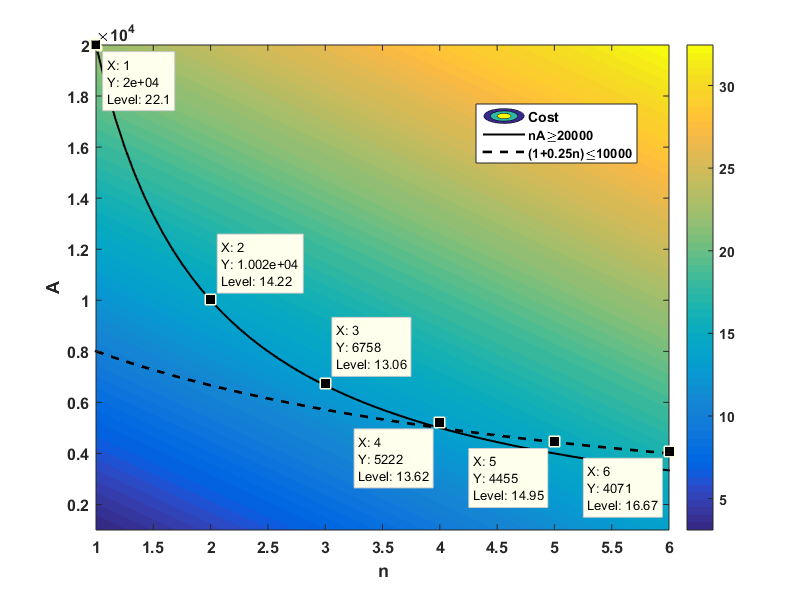
\includegraphics[width=\textwidth]{Graphics/aurora_p2-1.png}
\end{minipage}

\end{itemize}


%%%%%%%%%%%%%%%%%%%%%%%%%%%%%%%%%%%%%%%%%%%%%%%%%%%%%%
\newpage
\section{Thermodynamics}
\subsection{Background Mathematics}
\subsubsection{Exact Differential}
An exact differential is path independent and obeys the following rules for first and second derivatives
$$dz = \PartialConst{z}{x}{y}dx + \PartialConst{z}{y}{x}dy$$
$$\Partial{}{y}\Partial{z}{x} = \Partial{}{x}\Partial{z}{y}$$

\subsection{Classical Thermodynamics}
\subsubsection{The State Postulate}
\large\emph{The number of independent, intensive thermodynamic properties of a specified substance is equal to the number of relevant reversible work modes plus one. In the case of a simple compressible substance, two independent intensive properties are needed to completely define the thermodynamic state.}\\\normalsize

\textbf{Definition:} A simple substance is one for which there is only one reversible work mode. A simple compressible substance is one where that reversible work mode is fluid compression.\\

\textbf{Definition:} A reversible work mode is one where the the force is independent of direction and rate of change. The former implies the work done by a force $F$ in the direction $+dx$ is equal in magnitude to the work done by the same force in the direction $-dx$. Reversible work can be accounted for by reversible work plus heat transfer.\\

\textbf{Definition:} The free energy of a system (Helmholtz) is the energy available to do work. It is the difference between the total energy of the system and the energy which cannot be used for work, which is directly related to the entropy of the system. A similar definition holds for the free enthalpy (Gibbs).

\subsubsection{The First Law of Thermodynamics}
\large\emph{For a closed system where $dKE=dPE=0$, there exists a state variable $E$ such that, for an infinitessimal change in state,}
\CenteredBoxed{dE=\delta Q + \delta W}
\normalsize

\subsubsection{The Second Law of Thermodynamics}
\large\emph{There exists a state variable $S$ which can be produced but cannot be destroyed}
\CenteredBoxed{S_2-S_1=\Delta S \geq 0}
\normalsize

\textbf{Thermodynamic Definition of Temperature:}
Consider an isolated system split into two parts of constant volume which may interact. The entropy of the system can be expressed as 
$$S_C=S_A(U_A,V_A) + S_B(U_B,V_B)$$
Define the variable $\mu$ to track the progress of the thermal change of the system (assuming there is any) through heat transfer. Then we have the following
$$\frac{dS_C}{d\mu}=\PartialConst{S_A}{U_A}{V_A}\Partial{U_A}{\mu} + \PartialConst{S_B}{U_B}{V_B}\Partial{U_B}{\mu}$$
We know, from the second law of thermodynamics applied to isolated systems, that equilibirum is achieved when
$$\frac{dS_C}{d\mu}=0$$
Also, from the first law applied to isolated systems, we know
$$\frac{dU_C}{d\mu}=\frac{d}{d\mu}(U_A+U_B)=0$$
Therefore,
$$\PartialConst{S_A}{U_A}{V_A}=\PartialConst{S_B}{U_B}{V_B}$$
This allows us to define thermal equilibirum as the state at which the above equality holds. Furthermore, we can define temperature as the reciprocal of the rate of change of entropy with respect to internal energy at constant volume (reciprocal used such that heat flows from high to low temperatures).
\CenteredBoxed{T=\frac{1}{\left(\partial S/\partial U\right)_{V}}}

\textbf{Thermodynamic Definition of Pressure:}
Consider the same example as before but with the addition that the parts may exchange energy in the form of $pdV$ work.  Then we can define a new tracking variable $\mu_V$ which tracks the progress of the mechanical change of the system. Then
$$\frac{dS_C}{d\mu_V}=\PartialConst{S_A}{V_A}{U_A}\Partial{V_A}{\mu_V} + \PartialConst{S_B}{V_B}{U_B}\Partial{V_B}{\mu_V}$$
$$\PartialConst{S_A}{V_A}{U_A}=\PartialConst{S_B}{V_B}{U_B}\to p = T\PartialConst{S}{V}{U}$$

\textbf{The Gibbs Equation:}
For a simple compressible nonreacting substance we have the following
$$S = S(U,V)$$
$$dS = \PartialConst{S}{U}{V}dU + \PartialConst{S}{V}{U}dV$$
which, from our previous definitions, simplifies to
$$dS = \frac{1}{T}dU + \frac{p}{T}dV$$
or
\CenteredBoxed{dU = TdS - pdV}

\textbf{Entropy and Entropy Production:}
Consider a resevoir of fixed mass which maintains a constant temperature $T_r$. Then the Gibbs equation reduces to
$$dU = T_rdS$$
Consider a differential amount of heat being added to (or taken from) the resevoir. The first law states
$$dU = \delta Q\implies dS = \frac{\delta Q}{T_r}$$
Therefore we conclude that entropy can result from the exchange of heat.

Now consider two bodies, one at $T_A$ and the other at $T_B$ with $T_A<T_B$, which exchange an amount of heat $\delta Q$ (from B to A). Then the entropy change of each body is
$$dS_A =  \frac{\delta Q}{T_A}\geq0,\quad dS_B = - \frac{\delta Q}{T_B}\leq0$$
$$dS_B = -\frac{T_A}{T_B}dS_A$$
$$dS_{A+B} = dS_A + dS_B = dS_A\left(1-\frac{T_A}{T_B}\right)\geq0$$
Thus there is \emph{entropy generation within a system} due to heat transfer across finite temperature differences.

\subsubsection{Chemical Potential}
Previous results were obtained for a simple compressible substance of a single species. Now consider a mixture of simple compressible substances such that the entropy is a function of the two variables plus composition $S = S(U,V,n_1,n_2,...,n_k)$, and
$$dS = \PartialConst{S}{U}{V,n_i}dU + \PartialConst{S}{V}{U,n_i}dV + \sumlim{i=1}{k}\PartialConst{S}{n_i}{U,V,n_j}dn_i$$
$$dS = \frac{1}{T}dU + \frac{p}{T}dV - \sumlim{i=1}{k}\frac{\mu_i}{T}dn_i$$
Chemical potential is used to describe equilibrium of phase (or composition) in the same way temperature and pressure are used to describe thermal and mechanical equilibrium, respectively.

The chemical potential can be related to the Gibbs free energy in the following manner
$$G = G(p,T,n_i)$$
$$dG = \PartialConst{G}{p}{T,n_i}dp + \PartialConst{G}{T}{p,n_i}dT + \sumlim{i=1}{k}\PartialConst{G}{n_i}{p,T}dn_i$$
$$G = H - TS \implies dG = dH - TdS - SdT $$
$$dG = dU + pdV + Vdp - \left(dU - pdV -\sumlim{i=1}{k}\mu_idn_i\right) - SdT$$
$$dG = Vdp - SdT + \sumlim{i=1}{k}\mu_idn_i$$
Equating the second and last equations above results in the following
$$\PartialConst{G}{p}{T,n+i}=V,\quad\PartialConst{G}{T}{p,n_i}=-S,\quad\PartialConst{G}{n_i}{p,T}=\mu_i$$
This leads to the important result that the chemical potential of a pure substance of a single phase is equal to its molar Gibbs free energy.

Three possible criteria for equilibrium are:
\begin{enumerate}
\Item{Constant U and V} $dS = dU + pdV - \sumlim{i=1}{k}\mu_idn_i \geq 0$
\Item{Constant T and V} $dF = -SdT - pdV + \sumlim{i=1}{k}\mu_idn_i \leq 0$
\Item{Constant T and P} $dG = Vdp - SdT + \sumlim{i=1}{k}\mu_idn_i \leq 0$
\end{enumerate}
All three of these criteria require the following for equilibrium
\CenteredBoxed{\sumlim{i=1}{k}\mu_idn_i \leq 0}
That is, minimization of the sum of chemical potentials is a general requirement for equilibrium for multicomponent systems. We can apply this to simple reactions by defining a progress variable $\eta$ and finding its value such that the chemical potential of the system is minimized. Take the sample reaction $H_2 + Cl_2 \leftrightharpoons 2HCl$.
$$d\eta = \frac{dn_i}{\nu_i}$$
$$\nu_{H_2} = -1,\ \nu_{Cl_2} = -1,\ \nu_{HCl} = +2$$ 
$$\sum\mu_idn_i=\sum\mu_i(\nu_id\eta)=d\eta\left(\sum\mu_i\nu_i\right)\leq0$$
By convention $\eta\in[0,1]$ (i.e. $\eta=0$ if the composition is entirely LHS compounds and $\eta=1$ ifthe composition is entirely RHS compounds) so we require $\sum\mu_i\nu_i\leq0$. Therefore, if $\sum\mu_i\nu_i<0$ then the reaction will proceed from left to right (i.e. more of the positive $\nu$ compounds will be formed). Otherwise, if $\sum\mu_i\nu_i>0$ then the reaction will proceed form right to left (i.e. more of the negative $\nu$ compounds will be formed). Finally, if $\sum\mu_i\nu_i=0$ then equilibrium has been achieved (i.e. neither positive nor negaitve $\nu$ compounds are favored).

\subsubsection{Maxwell's Relations}
Maxwell's relations derive from the state postulate and the rules of exact differentials. Take, for example, the internal energy of a system
$$U = U(S,V)$$
$$dU = \PartialConst{U}{S}{V}dS + \PartialConst{U}{V}{S}dS$$
$$dU = TdS - pdV$$
then the second derivative rule for exact differentials requires
$$\PartialConst{T}{V}{S} = -\PartialConst{p}{S}{V}$$
We can perform similar operations on the enthalpy, Helmholtz free energy, and Gibbs free energy and arrive a similar results (these all assume $dn_i=0$)
$$dH = dU + d(pV) = TdS + Vdp \implies \PartialConst{T}{p}{S} = \PartialConst{V}{S}{p}$$
$$dF = dU - d(ST) = -SdT - pdV \implies \PartialConst{S}{V}{T} = \PartialConst{p}{T}{V}$$
$$dG = dH - d(TS) = -SdT + Vdp \implies -\PartialConst{S}{p}{T} = \PartialConst{V}{T}{p}$$

\subsubsection{Specific Heats}
We define the specific heats for a substance of known composition as follows:
$$dU = \PartialConst{U}{T}{V}dT + \PartialConst{U}{V}{T}dV$$
$$C_v = \PartialConst{U}{T}{V}$$

$$dH = \PartialConst{H}{T}{p}dT + \PartialConst{H}{p}{T}dp$$
$$C_p = \PartialConst{H}{T}{p}$$

Physically, these parameters specific how much heat must be added to the substance in order to increase its temperature by $dT$. Furthermore, using Maxwell's relations we can show
$$C_v = T\PartialConst{S}{T}{V},\quad C_p = T\PartialConst{S}{T}{p}$$

The units of the specific heats are energy per unit mass per unit change in temperature
$$C_x \equiv \mathrm{BTU/lbm \degree F} = \mathrm{cal/gK} = 4.187\ \mathrm{J/gK}$$

\subsubsection{Compressibility}
Compressibility cofficients are defined by expressing the volume of a substance as a function of its temperature and pressure
$$V= V(T,p)\implies dV = \PartialConst{V}{T}{p}dT + \PartialConst{V}{p}{T}dp$$
from which we deduce the isobaric and isothermal compressiblity coefficients
$$\alpha = \frac{1}{V}\PartialConst{V}{T}{p} = \frac{1}{T}\ \textrm{for an ideal gas}$$
$$\kappa = \frac{-1}{V}\PartialConst{V}{p}{T} = \frac{1}{p}\ \textrm{for an ideal gas}$$
where the division by volume means the compressibility coefficients correspond to fractional changes in volume per unit pressure or temperature. That is, $dV/V$ is something like a relative change in volume. We also have the isentropic compressibility
$$\beta=\frac{-1}{V}\PartialConst{V}{p}{S}$$

Note the negative signs, which indicate whether volume increases or decreases with an increase in the free variable (i.e. volumes tend to increase with temperature and decreasse with pressure).

Some interesting games can be played with the compressibility coefficients. First, note that the second derivative rule (reciprocity rule) for exact differentials applies, and thus requires
$$\PartialConst{\alpha}{p}{T} = -\PartialConst{\kappa}{T}{p}$$
Second, substituting the coefficients into the expression for volume, rearranging and integrating yields
$$\ln\left(\frac{V_2}{V_1}\right) = \alpha\Delta T - \kappa\Delta p$$
Third, from the cyclic rule, we have
$$\PartialConst{p}{T}{V}\PartialConst{T}{V}{p}\PartialConst{V}{p}{T}=-1\implies\PartialConst{p}{T}{V}=\frac{\alpha}{\kappa}$$
Lastly, by equating the differentials of $S(p,T)$ and $S(V,T)$, and applying Maxwell's relations (along with other results which have been shown along the way), we arrive at the following relationship
$$\PartialConst{p}{T}{V} = \frac{C_p-C_v}{T\PartialConst{V}{T}{p}} = \frac{\alpha}{\kappa}$$
$$C_p - C_v  = \frac{\alpha}{\kappa}T\PartialConst{V}{T}{p}=T\frac{\alpha^2V}{\kappa}$$
Which, for an ideal gas, reduces to the following result
\CenteredBoxed{C_p - C_v = \frac{pV}{T} = nR_u}
Since $n$, $T$, and $V$ must always be positive (and $R_u$ is positive) we see that $\kappa>0$ for all stable substances. Also, the difference between the specific heats goes to zero as the isobaric compressibility $\alpha$ or temperature $T$ go to 0 (experiments show that $\kappa\not\to0$). We can also show $C_p/C_v=\kappa/\beta$

\subsubsection{Imperfect Gases}
The definition of a perfect gas can be derived from quantum theory and statistical mechanics. It suffices to say a perfect or ideal gas obeys the law
$$p\nu=RT\implies \frac{p\nu}{RT}=1$$
Deviation from perfect gas behavior can be quantified by the compressibility factor $Z$
\CenteredBoxed{Z=\frac{p\nu}{RT}}

In general, compressibility curves collapse to well defined curves for reduced temperatures and pressures. Reduced properties are properties divided by their critical values (e.g. $T_r = T/T_{crit}$). The critical state is where liquid and gas phases coexist. The convergence of the curves is known as the principle of corresponding states. Maximum deviation from ideal behavior occurs at the critical values ($T_r=1$ and $p_r=1$). All gases tend towards ideal behavior at low pressures ($p_r\to0$) and high temperatures ($T_r\geq2$).

Imperfect behavior can also be characterized by their deviation from standard chemical potentials. This deviaiton is known as the fugacity and is defined as
$$\mu=\mu^0+R_uT\ln(f/f^0)$$
where the naught symbol implies the property is evaluated at the standard state. Fugacity has units of pressure and $f=p$ implies perfect gas behavior. Furthermore, $f/p\to1$ as $p\to0$ for all gases (this supports the above statements regarding the lower limit of the critical pressure).

The fugacity and compressibility are related via
\CenteredBoxed{\ln\left(\frac{f}{p}\right)=\intlim{0}{p}(Z-1)\frac{d\xi}{\xi}}
where the right hand side is evaluated with experimental data for the compressibility. With $Z=1$ for a perfect gas we have
$$\ln\left(\frac{f}{p}\right)=0\implies\frac{f}{p}=1$$

We can also define the partial fugacity for mixtures of imperfect gases
$$\mu_i=\mu_i^0 + R_uT\ln(f_i)$$
The partial fugacity will depend on pressure, temperature, and composition. We arrive at an analogous result for the relationship between partial fugacity and compressibility
\CenteredBoxed{\ln\left(\frac{f_i}{p_i}\right) = \intlim{0}{p}\left(\frac{\hat{\nu}_i}{R_uT}-\frac{1}{\xi}\right)d\xi}

If the interactions between components is not too strong (i.e. the density is not too high) then we can assume the result is similar to the ideal solution. The Lewis-Randall rule suggests
$$f_i=\chi_if^i$$
where $f^i$ is the fugacity of the pure substance at the mixture pressure and temperature.

\subsubsection{Equilibrium Constants}
In general, reactions can proceed in both the forward (left to right) and reverse (right to left) directions. For example, the reaction $H+O\leftrightharpoons OH$ implies atomic hydrogen and oxygen can collide to form a hydroxyl radical or, inversely, a hydroxyl radical may decompose into atomic hydrogen and oxygen. Equilibrium is achieved when the rates of the forward and reverse reactions are equal. The rates are not necessarily zero at equilibrium!\\

A series of equilibrium constants are defined for reactions which relate concentrations or partial pressures of each species involved, called concentration and pressure equilibrium constants, respectively. The concentration equilibrium constant is defined for a general stoichiometric reaction as follows
$$aA+bB+...\leftrightharpoons cC + dD +...$$
$$K_c = \frac{[A]^a[B]^b...}{[C]^c[D]^d]...}=\prod[\mathcal{S}_i]^{\nu_i}$$
where $[\mathcal{S}_i]$ is the molar concentration of the $i^{th}$ species and $\nu_i$ is its stoichiometric coefficient. The pressure equilibrium constant for the same general stoichiometric  is
$$K_p=\frac{p_A^ap_B^b...}{p_C^cp_D^d...}=\prod p_i^{\nu_i}$$
where $p_i$ is the partial pressure of the $i^{th}$ species. The pressure equilibrium constant can be rewritten with Dalton's law of partial pressures for an ideal gas, with $p$ the total pressure of the mixture, as
$$K_p=p^{\sum\nu_i}\prod\chi_i^{\nu_i}$$
This reflect Le Chatelier's principle; higher pressures favor the side of the reaction with the least moles. The two constants can be related, for a perfect gas, as
$$K_c = \sum[\mathcal{S}_i]^{\nu_i}=\sum\left(\frac{n_i}{V}\right)^{\nu_i}=\sum\left(\frac{n_i}{nR_uT/p}\right)^{\nu_i}$$
\CenteredBoxed{K_c = \left(\frac{1}{R_uT}\right)^{\sum\nu_i}\sum\left(p\chi_i\right)^{\nu_i}=\frac{1}{R_uT}K_p}

The equilibrium constants are defined for specific temperatures (and pressures). The magnitude of the constants indicate which side of the balanced reaction is ``favored'' at the given state. For example, high values ($\geq10^3$) of either constant indicate the right hand side (often the product side) is heavily favored. At unity, neither side is favored over the other; values close to zero ($\leq10^{-3}$) suggest the left hand side (often the reactant side) is favored.\\

The pressure equilibrium constant can also be defined for a perfect gas from the minimization of the chemical potential of the mixture. Recall
$$\mu_{mix} = \sum\mu_i=\sum\nu_i\mu_i^o + R_uT\sum\ln\left(\frac{p_i}{p^o}\right)$$
$$R_uT\sum\ln\left(\frac{p_i}{p^o}\right)=R_uT\ln\left(\prod\frac{p_i}{p^o}\right)=R_uT\ln(K_p)$$
$$\mathrm{Equilibrium}\implies d\mu_{mix}=0=d\left(\sum\nu_i\mu_i^o + R_uT\ln(K_p)\right)$$
All the terms on the right hand side are constants, therefore
\CenteredBoxed{\ln(K_p)=\frac{-1}{R_uT}\sum\nu_i\mu_i^o}
This equation shows the temperature dependence of the equilibrium constant(s), which we can investigate further by taking a derivative with respect to temperature
$$\frac{d}{dT}\left(\ln(K_p)\right) = \frac{d}{dT}\frac{-1}{R_u}\sum\nu_i\frac{\mu_i^o}{T}$$
$$\frac{d}{dT}\left(\frac{\mu_i^o}{T}\right) = \frac{-\hat{h}_i}{T^2}$$
$$\frac{d}{dT}\left(\ln(K_p)\right) = \frac{1}{R_u}\sum\nu_i\frac{\hat{h}_i}{T^2}$$
$$\sum\nu_i\hat{h}_i=\Delta\hat{H}_R$$
\CenteredBoxed{\frac{d\ln(K_p)}{dT} = \frac{\Delta\hat{H}_R(T)}{R_uT^2}}
This result is known as van't Hoff's equation. It states simply that the sensitivity of the (natural logarithm of the) equilibrium constant to temperature is equal to the molar enthalpy of the reaction at the current temperature divided by universal gas constant times the temperature squared. It assumes the system is a mixture of perfect gases (hence dropping the pressure dependence from the enthalpy of reaction). Note that the right hand side will be negative if the reaction is exothermic and positive if it is endothermic. Thus, as temperature goes up, an exothermic reaction will favor the left hand side while an endothermic reaction will favor the right hand side. This should make intuitive sense as higher temperatures implies a higher energy system, so reactions which require energy to proceed will see their rates increase whereas those which give off energy will have a harder time (think, where will the energy go?). The change in the equilibrium constant between two states can be found by integration
$$\intlim{1}{2}d\ln(K_p) = \intlim{T_1}{T_2}\frac{\Delta\hat{H}_R(T)}{R_uT^2}dT$$
It may be reasonable to assume the heat of reaction is (relatively) constant for small enough change in temperature. If this is the case, the following result is obtained
\CenteredBoxed{\ln\left(\frac{K_{p,2}}{K_{p,1}}\right) = \frac{\Delta\hat{H}_R(\bar{T})}{R_u}\left(\frac{1}{T_1}-\frac{1}{T_2}\right)}
where $\bar{T}$ can be $T_1$, $T_2$, or $\frac{1}{2}(T_1+T_2)$.\\

From the relationship between the equilibrium constants for a perfect gas, we have
$$\ln(K_c) = \ln(K_p) - \left(\sum\nu_i\right)\ln(R_uT) = \ln(K_p) - \Delta n \ln(R_uT)$$
$$\frac{d}{dT}\ln(K_c) = \frac{d\ln(K_p)}{dT} - \frac{d}{dT}\Delta n\ln(R_uT) = \frac{\Delta\hat{H}_R(T)}{R_uT^2} - \frac{\Delta n}{T}$$
$$\frac{d\ln(K_c)}{dT} = \frac{\Delta\hat{H}_R(T)-\Delta nR_uT}{R_uT^2} = \frac{\Delta\hat{H}_R(T)-\Delta(pV)}{R_uT^2}$$
\CenteredBoxed{\frac{d\ln(K_c)}{dT} = \frac{\Delta\hat{U}_R(T)}{R_uT^2}}

All of the above relationships have been derived \emph{assuming a perfect gas mixture}. The extension to imperfect gases uses the fugacity (rather than pressure) and is defined, via a similar manner as the pressure constant, as
$$\ln(K_f) = \ln\left(\prod f_i\right) = \frac{-1}{R_uT}\sum\nu_i\mu_i^o$$
where the reference state $f^0$ is chosen such that $f^0/p^0=1$ (i.e. a low pressure state). By choosing a low pressure we can approximate the system as a mixture of perfect gases, which implies the partial molar enthalpy is equal to the enthalpy of the pure substance at the same temperature (and is pressure independent) which allows us to write
$$\frac{d}{dT}\ln(K_f) = \frac{\Delta H_R^0}{R_uT^2}$$
where now the heat of the reaction must be taken at the reference pressure (hence the naught).\\

\noindent\textbf{Equilibrium Constants for Mechanisms}:\\

Consider the mechanism
\begin{align*}
A + B &\leftrightharpoons C & K_{p,1}\\
C + D &\leftrightharpoons E + F & K_{p,2}
\end{align*}
We could rewrite this as a single reaction 
$$A + B + D \leftrightharpoons E + F$$
with a third equilibrium constant $K_{p,3}$. With this, we see
$$K_{p,1} = \frac{p_C}{p_Ap_B},\quad K_{p,2} = \frac{p_Ep_F}{p_Cp_D},\quad K_{p,3} = \frac{p_Ep_F}{p_Ap_Bp_D}$$
$$K_{p,3} = K_{p,1}K_{p,2}$$
Therefore the overall pressure equilibrium constant is equal to the product of the individual reaction equilibrium constants.\\

For a mixture of $m$ species (compounds), consisting of $\alpha$ atomic nuclei, there are $m+2$ unknowns (need 2 thermodynamic properties). If the thermodynamic properties are specified along with the number or ratio of each atomic nuclei then there remain $m-\alpha$ unknowns, which can be found by using $m-\alpha$ independent $K_p$ expressions. This will set up a linear system which can be solved with appropriate techniques.

\subsection{Quantum Theory and Wave Mechanics}
\subsubsection{Bohr Model of the Atom}
After observing the discrete emission spectra for hydrogen atoms, Bohr postulated the following model for the atomic structure:
\begin{enumerate}
\item Atoms consist of heavy, positively charged nuclei and lighter, negatively charged electrons
\item Electrons orbit the nucleus in discrete orbits; only certain orbits are allowed which are stable. This suggests stationary quantum states as an orbiting electron, from classical mechanics, is accelerating
\item Frequency of emitted radiation (light) is governed by the change in orbital state $\nu=\Delta E/h$
\end{enumerate}

The second postulate lead to the assumption that angular momentum is quantized
\CenteredBoxed{L = m_ev_er = m_e\omega r = n\frac{h}{2\pi} = n\hbar}
where $n$ is the quantum number and $h$ is Planck's constant. Applying classical mechanics to balance the centripetal acceleration with the electrostatic force gives the following result (assuming circular orbits)
$$\frac{Ze^2}{r^2} = m_e\frac{v_e^2}{r}\implies Zm_ee^2r = L^2 = n^2\hbar^2$$

The total energy of an electron takes from in the kinetic and potential energies. Define the zero potential state such that $PE\to0$ as $r\to\infty$. Then
$$E = \frac{1}{2}m_ev_e^2 -\frac{Ze^2}{r} = \frac{Ze^2}{2r} - \frac{Ze^2}{r} = -\frac{Ze^2}{2r}$$
Employing theories of Planck and Einstein for emission spectra leads to the following (note $r_2 < r_1$)
\begin{align*}
\Delta E_{1\to2} = h\nu =& \frac{-Ze^2}{2}\left(\frac{1}{r_2}-\frac{1}{r_1}\right)\\
=& \frac{Ze^2}{2}\left(\frac{Zm_ee^2}{n_1^2\hbar^2}-\frac{Zm_ee^2}{n_2^2\hbar^2}\right)\\
=& \frac{2\pi^2Z^2m_ee^4}{h^2}\left(\frac{1}{n_1^2}-\frac{1}{n_2^2}\right)
\end{align*}
With $Z=1$ for a hydrogen atom, the distribution of wavelengths in the emission spectrum is
$$\frac{1}{\lambda}=\frac{\nu}{c} = \frac{2\pi^2e^4m_e}{h^3c}\left(\frac{1}{n_j^2} - \frac{1}{n_i^2}\right)$$
where the electron is jumping from state $i$ to state $j$ and $n_j < n_i$. (The emitted photon must have a positive amount of energy associated with it, so the electron must jump from a higher orbital to a lower one. If this were not the case, we would be looking at absorption spectra and the roles would simply be reversed.) This equation agrees well with the Balmer series of emission spectra ($n_j=2$) for atomic hydrogen.\\

\Header{Improvements to Bohr's Model}\\

The first improvement was to account for the motion of the electron about the center of mass, which is not necessarily the center of the nucleus. For this, we use the reduced mass
$$\mu = \frac{m_nm_e}{m_n+m_e},\quad \mu_H \approx 0.99945m_e$$

Clearly this has a small effect, especially on the simple hydrogen atom. It also does not account for the multiple observed lines within the Balmer series (better techniques had shown there to be three lines for the $n=2$ quantum level). This was account for by ditching the circular orbit assumption for elliptic orbits, which introduces an extra degree of freedom to the quantized energy. Application of Sommerfeld's action integral, which uses generalized momenta, yields both radial and azimuthal quantum numbers $n_r$ and $k$, respectively. Thus, for an elliptic orbit with major radius $a$ and minor radius $b$, we have
$$\frac{a}{b} = \frac{n_r+k}{k} = \frac{n}{k}$$
$$ a = \frac{\hbar^2}{\mu e^2}\frac{n^2}{Z},\quad b = \frac{\hbar^2}{\mu e^2}\frac{nk}{Z^2}$$

This, however, still did not fully account for the line splitting. That step required in the inclusion of Einstein's special relativity, which relates mass and velocity via the Lorentz factor as
$$m_{eff} = \frac{m_0}{\gamma} = \frac{m_0}{\sqrt{1+v^2/c^2}}$$
where $m_0$ is the mass at rest (i.e. zero velocity). This factor is important because electrons move very fast. Putting it all together yields the following, which permits (slightly) different energies for unique values of $n$ and $k$
$$E_{n,k} = -\frac{2\pi^2\mu e^4}{h^2}\frac{Z^2}{n^2}\left[1+\frac{\alpha^2Z^2}{n}\left(\frac{1}{k}-\frac{3}{4n}\right)\right]$$
where $\alpha = e^2/\hbar c\approx 0.0073$ is known as the fine structure constant. It was found, however, that there is a limitation on the changes in the azimuthal quantum number. Experiments suggests $k$ must change by one. That is, $\Delta k = \pm1$. Furthermore, the minimum value for $k$ is $n$, for which the orbit is circular.

\subsubsection{Quantized Energies: Translation}
Consider a free particle in a box. Schr{\''o}dinger's equation along any Cartesian direction reduces to that of a string with fixed boundary conditions, which leads to the result
$$E_{x_i} = \frac{h^2}{2m}\frac{n_i^2}{L_i^2}$$
Superposition of the three states gives
\CenteredBoxed{E_{trans} = \frac{h^2}{8m}\sum\frac{n_i^2}{L_i^2}}

\subsubsection{Quantized Energies: Rotation}
Consider a pair of atoms rotating about their center of mass. Schr{\''o}dinger's equation for this rigid system (i.e. constant radius) confined to a planar rotation provides the result
$$E_{\theta} = \frac{h^2n_{\theta}^2}{2I}$$
Expanding to three-dimensional rotation gives
\CenteredBoxed{E_{rot} = J(J+1)\frac{\hbar}{2I}}

\subsubsection{Quantized Energies: Vibration}
Consider a pair of atoms vibrating about their center of mass. Schr{\''o}dinger's equation for this harmonic oscillator gives
\CenteredBoxed{E_{vib} = h\nu\left(v+\frac{1}{2}\right)}

Note that even for a zero vibrational quantum ($v=0$) this system will poses \emph{some} vibrational energy. Also note the vibrational frequency does not change (i.e. $\nu = const$). Rather, it is the amplitude of the vibration which increases with the quantum number. Does this lead to dissociation at high energies?

\subsubsection{Quantized Energies: Electronic}
Consider a hydrogen atom: A nucleus with an electron orbiting it. It is possible for the system to store energy in the potential and kinetic energies of the electron. That is, the electron may gain energy and orbit at a greater radius while moving at a greater speed. There are three quantum numbers associated with this: the radial or principal quantum number $n$, the azimuthal or orbital angular moment quantum number $l$, and the magnetic quantum number $m$. There is also the spin quantum, which is always $\pm1/2$, as a result of being a Fermion.

\subsection{Statistical Mechanics}
\subsubsection{Enumeration of Microstates}
\subsubsection{Distribution over Microstates}

\subsection{Statistical Thermodynamics}
\subsubsection{The Maxwellian Velocity Distribution}
Collision theory requires a specific velocity distribution to satisfy the equilibrium rate condition (i.e. forward equals reverse). Considering bimolecular collision frequency and the application of conservation laws leads to closed form velocity distribution. The distribution is known as the Maxwellian velocity distribution and is described by
\CenteredBoxed{f_0(C)= \left(\frac{m}{2\pi kT}\right)^{1/2}\exp\left(\frac{-mC^2}{2kT}\right)}
The speed distribution (the magnitude of the velocity without consideration for direction) is then derived to be
\CenteredBoxed{\chi_0(C) = \left(\frac{m}{2\pi kT}\right)^{3/2}(4\pi C^2)\exp\left(\frac{-mC^2}{2kT}\right)}
The mode of the speed distribution is $\sqrt{2kT/m}$, while its mean is $\sqrt{8kT/\pi m}$, and the root-mean-square speed is $\sqrt{3kT/,}$. Note that there is zero probability of finding a particle with zero speed!
\begin{figure}[h]
\centering
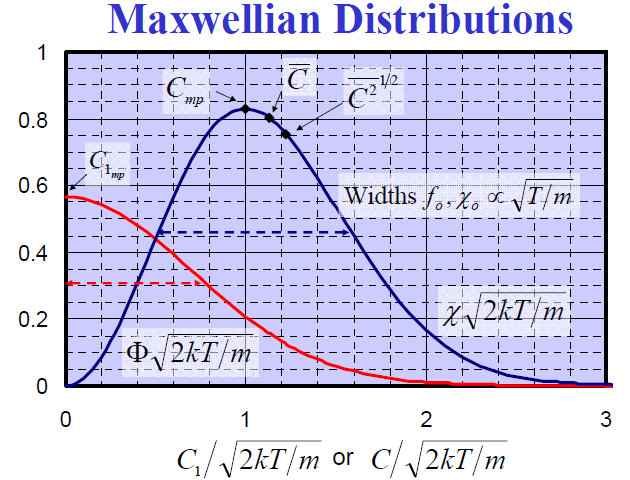
\includegraphics[scale=0.6]{Graphics/maxwellian_dist.PNG}
\end{figure}

%%%%%%%%%%%%%%%%%%%%%%%%%%%%%%%%%%%%%%%%%%%%%%%%%%%%%%

\section{Combustion}
\subsection{Chemical Kinetics}
\subsubsection{Basics}
Equilibrium thermodynamics considers where a reaction is heading if given enough time (i.e. the end states of a reaction) while kinetics considers the rates at which those changes occur (i.e. the intermediaries). For these rates we will typically define the non-dimensional Damk{\"o}hler number, which is the ratio of a characteristic flow time to a characteristic chemical time
$$Da = \frac{\tau_{flow}}{\tau_{chem}}$$
As the Damk{\"o}hler number goes to zero, the flow is said to be chemically frozen. Conversely, as it goes to infinity, the flow is said to posses fast kinetics.\\

Chemical kinetics depends on molecular collisions. The bimolecular collision frequency can be described as
$$\zeta_{AB} = n_An_B\sigma_{AB}\bar{V},\quad \bar{V}=\sqrt{\frac{8kT}{\pi\mu}}, \quad \sigma_{AB} = \pi d_{AB}^2,\quad d_{AB} = \frac{1}{2}(d_A+d_B)$$

Reaction rates are defined for both the forward and reverse reactions. They can be related by considering the equilibrium condition
$$A + B \leftrightharpoons C$$
$$\frac{d[C]}{dt} = -k_f[A][B] + k_r[C]= 0$$
$$\frac{k_f}{k_r} = \frac{[C]}{[A][B]} = K_c(T)$$
As the rates are not functions of composition, the relationship holds even for non-equilibrium conditions. Empirical results lead to the Arrhenius rate late for reaction rates as functions of temperature, shown here in its modified form
\CenteredBoxed{k = AT^b\exp\left(\frac{-E_A}{RT}\right)}
The activation energy can be found given the reaction rates (either forward or reverse, or both) at a specified temperature. this can be useful in determining if a reaction is endo- or exothermic (i.e. if $\Delta H = E_f-E_r$ is greater or less than zero). The magnitude of the activation energy correlates with the sensitivity of the reaction to temperature, as illustrated below.
\begin{figure}[h]
\centering
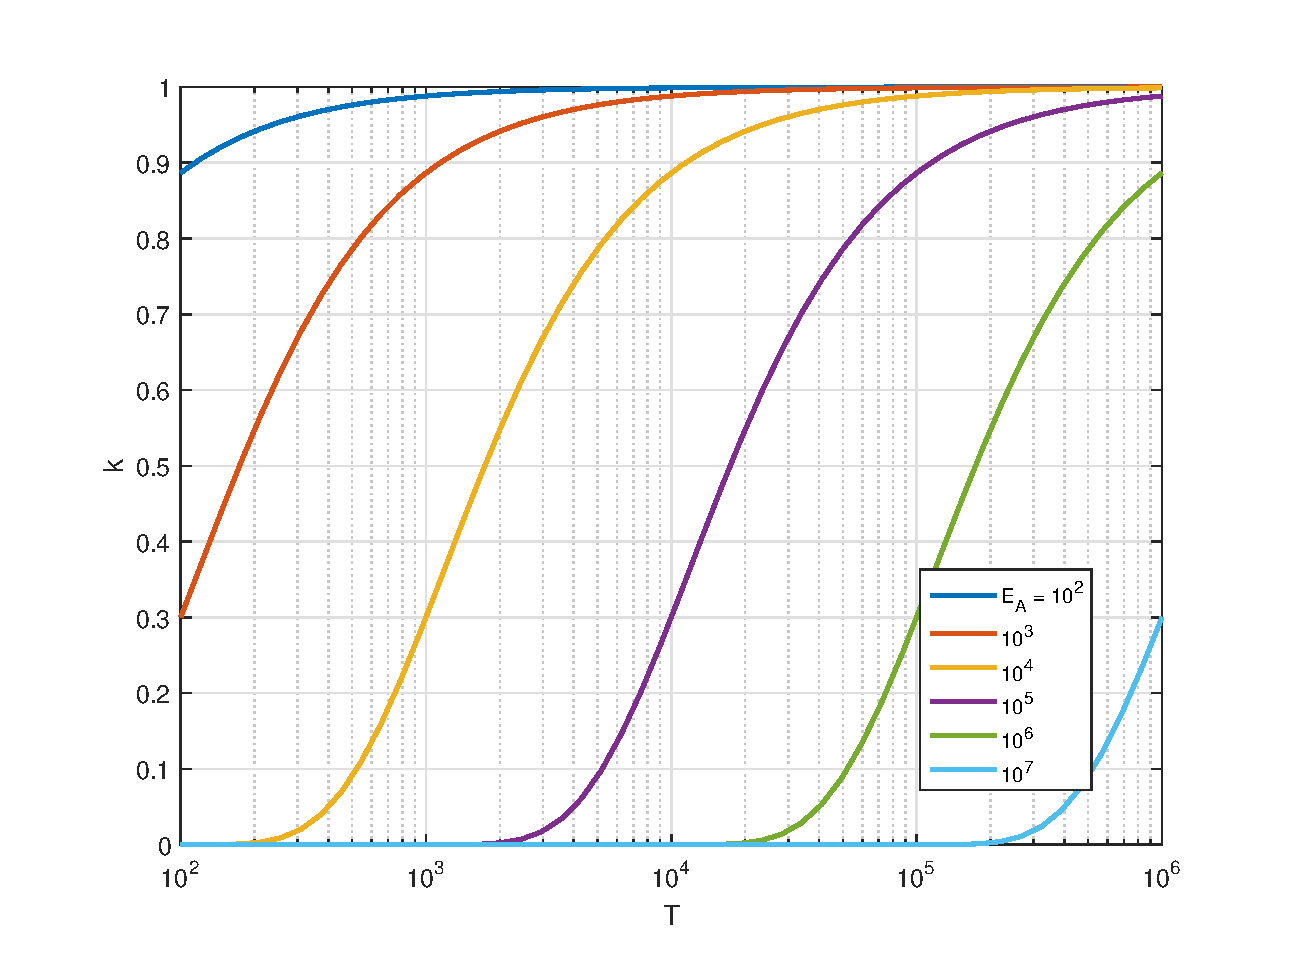
\includegraphics[width=0.7\textwidth]{Graphics/k_vs_T.eps}
\end{figure}

The pre-multiplying factor $A$ (along with the other $T$ dependence term) will affect the precise slopes and scales of the above graph, but the general idea is that higher activation energy reactions will not have high rates until adequately high temperatures are reached. Also note the log scaling of the ordinate: The change in $k$ for the $E_A=10^3$ case between approximately $T=175$ and $T=250$ is seen for the $E_A=10^5$ case between $T=1.6\times^4$ and $2.3\times10^4$. Thus, lower activation energy reaction rates are more sensitive to temperature changes, at least until the extremes are reached.\\

Reaction rates can be used, along with initial reactant compositions, to find characteristic chemical times. That is, for the above reaction, we could say
$$\tau_{chem} = \frac{[C]-[C]_0}{d[C]/dt}$$
If we assume the initial concentration of $C$ is almost zero and use the above rate constants, we get
$$\tau_{chem} = \frac{[C]}{k_f[A][B]}$$
These expressions get more interesting as the mechanisms become more complicated through dependencies on other species and/or reactions in the mechanism.\\

The partial equilibrium approximation is applied to \emph{reactions} within a mechanism (a system of reactions which approximate a process). The approximation fixes the (relative) concentrations of species' involved in the specified reaction to stoichiometric proportions and thus is only applicable to \emph{very} fast reactions (i.e. orders of magnitude faster than other mechanisms involving said species). It is also, in general, associated with energy neutral reactions, which do not require significant amounts of energy to proceed in either direction.\\

The steady state approximation is applies to \emph{species} within a mechanism or reaction. The approximation fixes the concentration of said species at some initial value and insists the rate of change of the concentration of said species is negligible compared to those of others (but not necessarily zero). That is, the concentration may change over time but it will not change as rapidly as the concentrations of other species will. This approximation is often applied to minor species, which tend to react quickly after forming (formation and destruction rates are close to one another).\\

Most reactions are sustained by radicals -- highly reactive compounds, typically with unpaired electrons. (The single step chemistry approximation ignores radicals.) Thus, overall reaction rates are dependent on the rapid production of these radicals. The initial formation of any radial is called the chain initiation step, which is often a highly endothermic reaction. It may be considered the first step in the reaction. Three paths may follow initiation, depending on the specific mechanism. Chain propagating reactions simply convert some radicals into other radicals. That is, the net number of radicals \emph{produced by the reaction} is zero. This step is often endothermic, though sometimes it may be energy neutral. Chain branching reactions convert some radicals into more radicals, resulting in a net gain of radicals. Chain branching reactions are often exothermic, albeit only slightly. Chain terminating reactions take in a radical and put out non-radical compounds (i.e. stable compounds or, often, products), resulting in a net loss of radicals. Chain terminating reactions are, in the case of exothermic overall reactions, highly exothermic and are where the bulk of the heat release comes from. Chain termination may occur via bimolecular collisions or wall collisions.\\

True reactions are mechanisms composed of vast networks of reactions, each interacting and/or competing for species'. The more accurate mechanisms may contain hundreds of reactions and as many species, sometimes more. The complexity of these mechanisms renders hand calculations futile and requires (super-) computer capabilities. That being said, some simple mechanisms can be considered to get familiar with the concepts.\\

Consider carbon monoxide oxidation (burnout)
$$CO + \frac{1}{2}O_2 \to CO_2$$
This is a highly exothermic reaction with an adiabatic flame temperature close to 3000K (indeed, $CO$ burnout is responsible for most of the heat release in alkane combustion, per Turns). Dry $CO$ burnout, where there are no hydrogen species present, are very slow at combustion temperatures. The mechanism is vastly accelerated by adding hydrogen species' to the mix. The reason for the increase is the number of paths hydrogen-containing compounds open up for the formation of $CO_2$, mostly through the availability of the hydroxyl radical $OH$. This is particularly relevant because hydrogen chemistry is faster than $CO$ chemistry, which means the $CO$ are not waiting around for high energy diatomic oxygen or even higher energy atomic oxygen, but can collide with the abundant hydroxyl radicals. Furthermore, the reaction involving hydroxyl radical is chain propagating and therefore does not harm the radical concentrations (it converts an $OH$ to and $H$, which can then go on to react with other things).\\

\Header{NOx Mechanisms}\\

These mechanisms are important because $NO$ goes on to form $NO_2$ in the atmosphere, which is responsible for acid rain and photochemical smog. Thus designers are often concerned with $NO$ production and how it can be mitigated. Perhaps the most widely used $NO$ mechanisms is that of Zeldovich
$$N_2 + O \leftrightharpoons NO + N$$
$$O_2 + N \leftrightharpoons NO + O$$
This reaction is rate-limited by the first reaction, which is endothermic, and works fairly well for dry, lean combustion at high temperatures and moderate residence times. An extension to this basic mechanism increases its accuracy for wet systems (i.e. where hydrogen species' are present). The added reaction, which is exothermic like the second reaction, is
$$OH + N \leftrightharpoons NO + H$$
The first reaction is still rate limiting. The Zeldovich mechanism and its extended version are \emph{thermal} mechanisms; they dominate at high temperatures in lean environments, typically require long residence times, and are sensitive to $O$ and $OH$ radical concentrations.\\

An mechanism was derived for explaining low temperature, lean combustion systems. The mechanism uses $N_2O$ as an intermediate between $N_2$ and $NO$ as follows
$$N_2 + O (+ M) \leftrightharpoons N_2O (+ M)$$
$$N_2O+H \leftrightharpoons NO + NH$$
$$N_2O + O \leftrightharpoons 2NO$$
Additional reactions which compete for intermediate species include
$$N_2O + H \leftrightharpoons N_2 + OH$$
$$N_2O + O \leftrightharpoons N_2 + O_2$$
$$N_2O + OH \leftrightharpoons N_2 + HO_2$$
$$NH + O \leftrightharpoons NO + H$$
$$NH + O_2 \leftrightharpoons NO + OH$$

\subsection{Reactor Models}
The use of reactor models is motivated by the need to couple the chemical kinetics problem with the temperature and pressure of the system -- two intensive variables which are relatively easy to measure. This need arises from the interdependence of the chemical kinetics on temperature and pressure which, in general, requires simultaneous solution of mass, momentum, and energy conservation, along with state equations. Chemical reactions will affect temperature and those two will affect the pressure, while mixing will have an impact on the local mole (or mass) fractions, which drive chemical reactions. For these systems we define the molar production rate as the rate of change of concentration for a given species
\CenteredBoxed{\dot\omega_i = \frac{d[M_i]}{dt}\equiv\frac{mole}{m^3s}}
The mass production rate is linked to this via the volume and molar weight
$$\dot m_i = V\bar{W}\dot\omega$$
These production rates are directly coupled with the temperature via the specific heat and enthalpy of reaction
$$m\frac{dh}{dt} = V\dot q'''_{chem} + c_{p_{mix}}\frac{dT}{dt}$$
$$\frac{dh}{dt} = \frac{V}{m}\sum\bar h_i(T)\dot\omega_i + \frac{1}{m}\left(V\sum[M_i]\bar c_{p_i}\right)\frac{dT}{dt}$$
$$\bar h_i(T) = \Delta\bar h_{f,T_{ref},i}^o + \intlim{T_{ref}}{T}\bar c_{p_i}dT$$

Reactor models allow us to ignore the mixing dependence/coupling and focus solely on the energy/species coupling. Recall the Damk{\''o}hler number and its limits
\begin{align*}
Da &= \frac{\tau_{mix}}{\tau_{chem}}\\
Da&\to0\implies\textrm{fast mixing, uniform fluid}\\
Da&\to\infty\implies\textrm{no mixing}
\end{align*}
Chemical reactors may be closed (batch reactor), where the mass of the system is fixed at either constant pressure or constant volume, or open (flow reactor), where mass flows through the system. Closed, constant volume systems are good for analyzing fast reactions such as those in internal combustion engines. Closed, constant pressure systems allows for $pdV$ work, which changes the energy equation and thus modifies the coupling. Both reactor models follow the same ordinary differential equations for species, which simply equates the molar production rate to the difference between the production and destruction rates for each reaction involving said species
$$\dot\omega_i=\frac{d[M_i]}{dt} = (\nu_{ji}''-\nu_{ji}')\left[k_{j,f}\prod[M_i]^{\nu_{ji}'}-k_{j,r}\prod[M_i]^{\nu_{ji}''}\right]$$
The energy coupling depends on which type of system is analyzed. Constant pressure systems utilize the enthalpy of the system
$$\rho\bar c_p\frac{dT}{dt} = \dot q'''_{ext}(t) - \sum\bar h_i(T)\dot\omega_i$$
while constant volume systems utilize the internal energy, which can be found by the definition of enthalpy (note that enthalpy is what is used to describe the heat of reactions, which is why it appears here)
$$h = e + pv \implies \frac{dh}{dt} = \frac{de}{dt} + \frac{d(pv)}{dt} = \frac{de}{dt} + p\frac{dv}{dt} + v\frac{dp}{dt}$$
$$p\frac{dv}{dt} = 0,\quad v\frac{dp}{dt} = v\frac{d}{dt}\left(\frac{R_{mix}T}{v}\right)=R_{mix}\frac{dT}{dt} + T\frac{dR_{mix}}{dt}$$
$$\frac{de}{dt} = \frac{dh}{dt} - \left(R_{mix}\frac{dT}{dt} + T\frac{dR_{mix}}{dt}\right)$$
$$\rho\bar c_v\frac{dT}{dt} = \dot q'''_{ext}(t) - \sum\bar e_i(T)\dot\omega_i$$
where the last step was made by rearranging and combining like terms to convert the $c_p$ term to $c_v$. In both equations,
$$\bar c_p = \sum Y_i(t)c_p(T(t))$$

\subsubsection{Plug Flow Reactor}
Plug flow reactors are simple, steady, 1D flow reactor models. The 1D assumption means properties may only vary along the flow direction, with no axial diffusive transport ($Da_x\to\infty$) or cross-stream variations. Furthermore, the walls assumed to be non-reacting and the system is assumed to be non-accelerating. These assumptions lead to the following set of governing equations
\begin{align*}
\textrm{Conservation of Mass: } &\frac{d(\rho u_xA)}{dx} = 0\\
\textrm{Conservation of Energy: } &\rho u_x\bar c_p \frac{dT}{dx} = \dot q'''_{in} - \sum h_i\dot\omega_i\\
\textrm{Conservation of Momentum: } &(\rho u_xA)\frac{du_x}{dx} = -A\frac{dp}{dx} - \tau_wP\\
\textrm{Conservation of Species: } &(\rho u_x)\frac{dY_i}{dx} = \bar W_i \dot\omega_i
\end{align*}

\Header{Conservation of Mass}\\

The equation for conservation of mass simply states that there is no mass destruction or creation along the length of the reactor. If the reactor has a non-constant cross sectional area then the density and axial velocity terms must vary such that the mass flux through any cross section is constant. This couples all the other conservation equations.

For the case of constant cross sectional area, the mass conservation equation reduces to
$$\frac{d}{dx}(\rho u_x) = 0$$
Typically, the larger effect is to increase the axial velocity and decrease density, rather than the other way around (reduce axial velocity and increase density).\\

\Header{Conservation of Energy}\\

The left hand side the energy equation represents the transport of heat (energy) in the flow direction via mass (convection). It requires the temperature to remain constant for a non-reacting, adiabatic system, which is expected. For a reacting adiabatic system (i.e. first term on right hand side is zero) the heat released by the reactions must be convected downstream. Alternatively, for an endothermic process, the energy required for the reaction must come from upstream via convection. The lack of a diffusive term -- which would make this a second order ODE -- means the only way heat can move around is by convection.

Adding or removing heat from the system (i.e. non-zero first term on right hand side) would have a significant impact on the temperature profile. Adding heat could push the mixture to ignition, while removing heat could prevent the mixture from igniting at all. Whether or not either of these things would happen depends on the precise heat flux profile (i.e. volumetric heat flux as a function of axial location) and the inlet conditions.

\Header{Conservation of Momentum}\\

The left hand side of this equation is the convection of momentum. Recall that the term in parentheses is the mass flux, the spatial gradient of which is necessarily zero according to the first conservation equation (mass). The first term on the right hand side is a pressure gradient term, while the last term is viscous dissipation at the wall in the form of the shear stress times the length of the perimeter.

This equation is very similar in form to Bernoulli's equation (really Euler's equation, as it is in differential form), which is no coincidence. Conservation of momentum is a standard (necessary) conservation equation for flowing systems.

\Header{Conservation of Species}\\

The left hand side of this conservation equation is the convection of species mass fraction in the flow direction. The right hand side of the equation is the molar production rate (as a function of axial location) times the molar mass of said species. There is one species conservation equation per species involved in the overall mechanism.\\

\noindent\rule{\textwidth}{0.4pt}\\
\noindent\rule{\textwidth}{0.4pt}\\[0.3cm]

Molecules in the gas collide as they move from one end of the reactor to the other. These collisions may or may not be sufficient in frequency and energy to begin the combustion process, as we only consider the processes which take place within the reactor. If the gas remains within the reactor long enough for rapid radical buildup to take place then the fluid particles will accelerate as a result of the heat release (which leads to expansion). The residence time -- the time a fluid packet spends inside the reactor -- decreases as the bulk velocity increases (plug flow reactors have a fixed, finite length).\\

The induction time or autoignition delay is an important metric for plug flow reactors. Induction time is the time delay between the gas entering the reactor and the start of combustion. The precise definition of when combustion begins is not trivial; a convenient point to take is the knee of the temperature profile versus residence time (maximum curvature). The residence time may be compared to a characteristic chemical time
$$\tau_{chem} \propto \frac{1}{k} = \exp\left[E_A/RT\right]$$
$$\ln(\tau_{chem})\propto\frac{1}{T}$$
If the residence time is much less than the characteristic chemical time then it is unlikely the reactor will contain any (significant) reactions. Conversely, if the chemical time is much less than the residence time then the gas will likely ignite very early in the process and approach equilibrium at the exit. These are the limits of the Damk{\"o}hler number for plug flow reactors
$$Da_{PFR} = \frac{\tau_{res}}{\tau_{chem}}$$

\Header{Effects on Autoignition Delay}\\

Pressure has an approximately inverse effect of autoignition delay
$$\frac{\tau_{chem}}{\tau_{chem,0}} \approx \frac{p_0}{p}$$
For example, if the pressure is increased by a factor of 10 then the induction time will decrease by approximately a factor of 10. This is mostly a result of the increase in collision frequency which comes with higher pressure. More collisions means a higher likelihood of all chain reactions (initiation, branching, propagation, and termination).\\

Equivalence ratio has a nearly negligible effect on the autoignition delay. The effects of temperature and pressure are far more significant than that of equivalence ratio. There is a small effect; the delay time will decrease slightly with increasing equivalence ratios, particularly for colder inlet temperatures, but the change is so small it can be ignored.

\subsubsection{Well/Perfectly Stirred Reactor}
Well- or perfectly-stirred reactor models are useful for examining highly mixed engines, low pressure combustion systems, low speed reactors (fast diffusion), turbulent parts of non-premixed combustion, residence time issues, and high temperature chemical kinetics. They rely on the assumption that the Damk{\"o}hler number for mixing is much less than one (i.e. very, very fast mixing). Inlet conditions are specified (mass flow rate, temperature, species mass fractions) and the fast mixing assumption means the interior and outlet conditions are the same. Thus the properties at the outlet are dependent on the resident time within the reactor, which is given by the conservation of mass
$$\frac{d}{dt}m_{sys} = 0\implies \tau_{res} = \frac{\rho V}{\dot m_{in}}$$
The governing equations are then
\begin{align*}
\textrm{Conservation of Mass: } &\frac{d(\rho V)}{dt} = \dot m_{in} - \dot m_{out}\\
\textrm{Conservation of Energy: } &\bar c_p\frac{dT}{dt} = \frac{\dot m_{in}}{\rho V}\sum Y_{i,in}(h_{i,in}-h_i) - \frac{1}{\rho}\sum h_i\dot\omega_i\bar W_i  + \frac{q'''_{in}}{\rho}-\frac{1}{\rho}\frac{dp}{dt}\\
\textrm{Conservation of Species: } &\frac{dY_i}{dt} = \frac{\dot m_{in}}{\rho V}(Y_{i,in}-Y_i) + \frac{\dot\omega_i\bar W_i}{\rho}
\end{align*}

\Header{Conservation of Mass}\\

The left hand side is the time rate of change of the mass contained within the reactor, while the right hand side is the difference between the inlet and outlet mass fluxes. This is a direct application of Reynold's Transport Theorem to the control volume enclosing the reactor. Only one inlet is considered because of the well-stirred assumption, which would see the two streams completely and instantaneously mixed upon entering the reactor. The steady assumption drives the difference to zero and thus $\rho V = const.$.

\Header{Conservation of Energy}\\

The left hand side of the equation is the time rate of change of heat contained within the system (the $\bar c_p$ term is a function of composition, and thus, possibly, a weak function of time). The first term on the left hand side is the difference in enthalpy between the inlet and outlet states. The second term is the enthalpy of formation for each species, in the form of the specific enthalpy and the mass production rate of that species. This accounts for both the destruction of reactants and the formation of products (recall that enthalpy of formation is negative for exothermic reactions and positive for endothermic reactions). The third term is volumetric heat addition, while the last is a work term. We may assume a well-stirred reactor to be isobaric and thus can neglect this term.

\Header{Conservation of Species}\\

The left hand side is the time rate of change of the mass fraction of each species contained within the reactor. The first term on the right hand side is the difference in mass fractions between the inlet and outlet streams ($\dot m_{in} = \dot m_{out}$ and $Y_i = Y_{i,out}$), while the second term is the destruction/formation term from chemical reactions.

\noindent\rule{\textwidth}{0.4pt}\\
\noindent\rule{\textwidth}{0.4pt}\\[0.3cm]


Some simplifying assumptions for well-stirred reactors include the steady operation assumption, which requires all the time derivatives to be zero. This reduces the system to an algebraic one. Another useful assumption is the constant and uniform mixture specific heat. This assumption simplifies the energy equation, particularly for transient problems. Finally, single step chemistry may be useful. The single step approximation implies
$$\tau_{mix} << \tau_{chem} << \tau_{res}$$
the latter of which may generally be true. The Damk{\"o}hler number associated with the residence and chemical times is extremely important for well-stirred reactors. The question of whether or not the reactor will ignite or extinguish is precisely a question residence vs chemical times. Higher activation energies -- and thus longer chemical times -- will require longer residence times before combustion can occur. These higher $E_A$ reactions will be more sensitive to inlet temperature than their low $E_A$ counterparts, which will see at least partial combustion as most reasonable inlet temperatures.

The effect of pressure on PSR outlet conditions is similar to that on a PFR. Higher pressure means higher collision frequencies, which decreases the autoignition delay. The increase in pressure will also push the mixture closer to complete combustion (assuming it has ignited) by Le Chatelier's principle.

\subsection{Premixed One-Dimensional Combustion Waves}
Consider a flame to be a sheet with reactants moving into the flame from one side and products leaving it from the other. Here we are assuming infinitely fast, single-step chemistry (i.e. the flame has no thickness). The standard conservation equations -- mass, energy, momentum, and species -- all still apply to a control volume placed around the flame. Doing this control volume analysis allows us to ignore (for now) the specifics of what is happening inside the flame and concern ourselves only with the properties of the incoming reactants and outgoing products.
%\textrm{Conservation of Energy: } &h_{1,s} + \frac{1}{2}u_1^2+q = h_{2,s} + \frac{1}{2}u_2^2\\
%\textrm{Conservation of Species: } &(\rho u_x)\frac{dY_i}{dx} = \bar W_i \dot\omega_i

\subsubsection{Rayleigh Line}
Consider the conservation of mass applied to the control volume
$$\frac{d(\rho u_xA)}{dx} = 0$$
The dimensionality of the problem reduces this to
$$\frac{d(\rho u)}{dx} = 0\implies\rho_1u_1=\rho_2u_2=\dot m''$$
Furthermore, we can neglect the shear stress term in momentum conservation to get
$$p_1+\rho_1u_1^2 = p_2+\rho_2u_2^2$$
Substituting mass conservation into momentum conservation gives
$$p + \dot m''^2/\rho = const.\to p = -\dot m''^2\left(\frac{1}{\rho}\right)$$
\CenteredBoxed{\frac{dp}{d(1/\rho)} = -\dot m''^2}
This linear relationship between the pressure and specific volume (inverse of density) is known as the Rayleigh line.

\subsubsection{Rankine-Hugoniot}
Energy conservation is applied via the Reynolds Transport Theorem
$$\frac{d}{dt}E = \frac{d}{dt}\intlim{\Omega}{}\rho edV + \intlim{\partial\Omega}{}\rho e(v\cdot n)dS$$
The energy of the system consists of the enthalpy and kinetic energy of the gas, and there is no work or heat being added to the gas as it flows across the flame (it is releasing heat, though), so conservation of energy reduces to
$$h_1 + \frac{1}{2}u_1^2 = h_2 + \frac{1}{2}u_2^2$$
Assuming the stagnation enthalpy is constant (because no work is being done) we can express the enthalpy in terms of the sensible and chemical forms
$$h = h_s + h_c$$
The reactants release their chemical energy upon combusting, converting that enthalpy from chemical to sensible form in the products as the heat of reaction
$$h_{1,s} + q = h_{2,s}$$
This gives the final form of energy conservation as
$$h_{1,s} + \frac{1}{2}u_1^2 + q = h_{2,s} + \frac{1}{2}u_2^2$$
We have the difference in squared velocity from momentum conservation
$$p_2-p_1 = \dot m''\left(\frac{1}{\rho_1}-\frac{1}{\rho_2}\right) = (\rho_1u_1)^2\left(\frac{1}{\rho_1}-\frac{1}{\rho_2}\right) $$
\begin{align*}
u_1^2 &= \frac{1}{\rho_1^2}\left(\frac{p_2-p_1}{1/\rho_1-1/\rho_2}\right)\\
u_2^2 &= \frac{1}{\rho_2^2}\left(\frac{p_2-p_1}{1/\rho_1-1/\rho_2}\right)\\
u_1^2-u_2^2 &= \left(\frac{1}{\rho_1^2}-\frac{1}{\rho_2^2}\right)\left(\frac{p_2-p_1}{1/\rho_1-1/\rho_2}\right)\\
u_1^2-u_2^2 &= \left(\frac{1}{\rho_1}-\frac{1}{\rho_2}\right)\left(\frac{1}{\rho_1}+\frac{1}{\rho_2}\right)\left(\frac{p_2-p_1}{1/\rho_1-1/\rho_2}\right)\\
u_1^2-u_2^2 &= (p_2-p_1)\left(\frac{1}{\rho_1}+\frac{1}{\rho_2}\right)
\end{align*}
Now we make the calorically and thermally perfect gas assumptions, which are not a bad assumption because the incoming gases will be at a relatively low temperature and the outgoing gases will be at a relatively high temperature. Thus we can express the change in sensible enthalpy as
$$\Delta h_{1\to2,s} = c_p\Delta T_{1\to2} = \frac{\gamma}{\gamma-1}\left(\frac{p_2}{\rho_2}-\frac{p_1}{\rho_1}\right)$$
Combining the results for velocity and sensible enthalpy into the basic energy conservation equation yields
$$q = \Delta h_{1\to2,s} - \frac{1}{2}\Delta u_{1\to2}^2$$
\CenteredBoxed{q = \frac{\gamma}{\gamma-1}\left(\frac{p_2}{\rho_2}-\frac{p_1}{\rho_1}\right) - \frac{1}{2}(p_2-p_1)\left(\frac{1}{\rho_1}+\frac{1}{\rho_2}\right)}

This defines a rectangular hyperbola, known as the Rankine-Hugoniot line. It combines mass, energy, and momentum conservation principles into a single equation. Positive heat (exothermic) pushes the hyperbola up and to the right, while negative heat (endothermic) pushes it down and to the left. No heat release gives the solution for a non-reacting shock Hugoniot.
\begin{figure}[h]
\centering
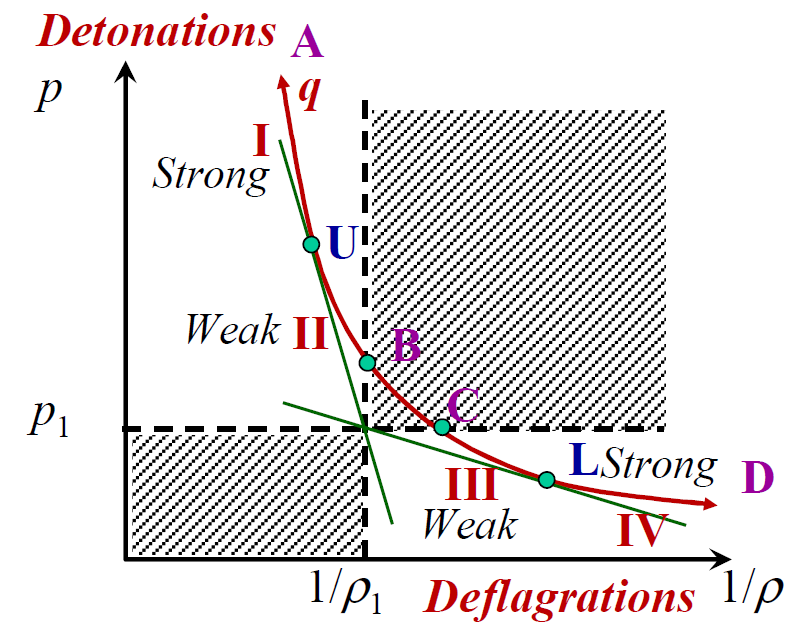
\includegraphics[scale=0.5]{Graphics/detonations_deflagrations.PNG}
\end{figure}

\subsubsection{Allowed Solutions}
The solution to a given 1D flame problem is found at the intersection of the Rankine-Hugoniot and Rayleigh lines. There are two points where there is exactly one solution, known as the upper and lower Chapman-Jouguet points. For all other cases there are multiple intersections, all but one of which are eliminated on the basis of the second law of thermodynamics. Applied to flowing systems in the absence of work, the second law of thermodynamics requires flows to accelerate towards the local sound as heat is added.

\begin{itemize}
\Item{Strong Detonations} Possible, but unlikely. Expansion events downstream could propagate upstream, decreasing the pressure behind the flame and slowing it down until it reaches Mach 1.
\Item{Upper CJ Point} Defines the CJ detonation, where the velocity of the product gases is the local sound speed. It is also the minimum wave speed for detonations, since it has the least negative slope of any detonation.
\Item{Weak Detonations} Product gases are supersonic. This violates the second law according to the structure of the flame.
\Item{Weak Deflagrations} Totally possible. Subsonic on both sides of the flame.
\Item{Lower CJ Point} Defines the CJ deflagration. The velocity of the product gases at this point is also the local sound speed, and it is the maximum allowed wave speed for deflagrations (most negative slope).
\Item{Strong Deflagrations} Reactants are subsonic but products are supersonic. Direct violation of second law.
\end{itemize}


\subsubsection{Planar Detonations}
Planar detonations can be model with the Zeldovich-von Neumann-D\{"o}ring structure, which suggests detonations consist of leading shocks followed by a zone of chemical reactions. This is based on the general idea that collisions which equilibrate pressure and translational energies precede chemical reactions, since their characteristic times differ by orders of magnitude. The leading shock sharply increases the pressure and temperature behind it, reducing the necessary induction time for the reactions to take place. It also makes the post-shock flow subsonic, which is why weak detonations were not permitted (cannot go supersonic again without work). What follows the shock looks much like a deflagration since the flow is subsonic on both sides of the flame.

\begin{figure}[h]\centering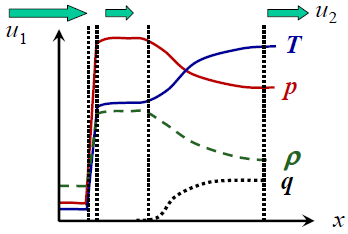
\includegraphics[scale=0.8]{Graphics/znd_structure.PNG}\end{figure}

Solving for the detonation wave speed $D\equiv u_1$ can be done by coupling the CJ constraint $u_2=a_2$ with mass conservation and the solutions from the Rayleigh line. Doing so gives
\CenteredBoxed{D=\frac{\gamma_2+1}{\gamma}\sqrt{\frac{\gamma_2T_2R_u}{\overline{W}_2}}}
The $T_2$ factor captures the heat release effect on detonation wave speed, while the average molecular weight $\overline{W}_2$ captures the effect of product composition as well as reactant equivalence ratio.

\subsection{Laminar Premixed Flames}
Weak deflagrations exist across their whole range, so now we seek to characterize the wave speed for these phenomena. The weak deflagration wave speed is known as the laminar flame speed $S_L^0$.
\begin{figure}[h]\centering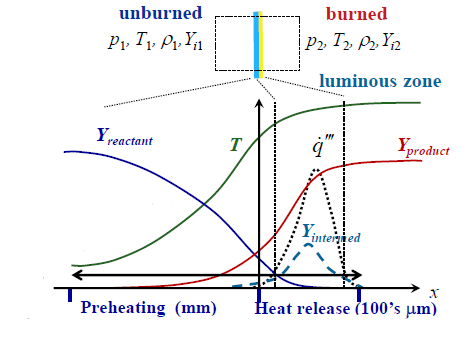
\includegraphics[scale=0.8]{Graphics/laminar_flame_structure.PNG}\end{figure}

\subsubsection{Laminar Flame Speed}
Investigating laminar flame speed requires more detailed analyses than were previously employed; control volume analysis is insufficient for understanding how laminar flames actually propagate. We can break down the laminar flame into a basic two-zone structure: the preheat zone and the reaction/heat release zone. The preheat zone precedes any significant reactions; the zone is characterized by heat and species diffusing upstream. This upstream diffusion helps the flame propagate, effectively priming the incoming reactants for the reaction zone, where basically all the heat release happens. Finite gradients exist in this two-zone structure, further emphasizing the importance of diffusive processes in laminar flame propagation.\\

Based on the shape of the Rankine-Hugoniot curve we can assume laminar flames are approximately constant pressure processes ($p_2$ is slightly lower than $p_1$ but we can neglect this for low fidelity analyses). This reduces our conservation equations for mass and momentum, respectively, to
$$\frac{d(\rho u)}{dx} = 0\quad \frac{d(\rho u u)}{dx} = 0$$
we must, however, include diffusion in the energy and species conservation equations
$$\dot m''\frac{dY_i}{dx} = -\frac{dj_{i,x}}{dx} + W_i\dot\omega_i$$
$$\dot m''c_p\frac{dT}{dx} = \frac{d}{dx}\left(\lambda\frac{dT}{dx}\right) - \sum c_{p,i}j_{i,x}\frac{dT}{dx} - \sum h_i\dot\omega_iW_i$$

\Header{Explanation of Terms}\\

The left hand side of each equation represents convection of said quantity via bulk flow. The first term on the right hand side of the species equation is the gradient of the diffusive mass flux through the flow. The negative sign is there because species' diffuse from high concentrations to low concentrations, so if the gradient of the mass fraction of a species is positive then the gradient (increasing along $x$) of the diffusive velocity is in the negative direction. The second term is the molar production rate times the molecular mass.

The first term on the right hand side of the energy equation is the gradient of the conduction term ($\lambda\equiv k$). The second term is the convection of heat through diffusion (as opposed to that through bulk flow), and the last term is the production rate of enthalpy via chemical reactions.\\

Rearranging the equations and substituting some terms results in the Shvab-Zeldovich energy formulation
$$\frac{d}{dx}\left[\dot m''Y_i - \rho D\frac{dY_i}{dx}\right] = W_i\dot\omega_i$$
$$\frac{d}{dx}\left[\dot m''h_s -\rho\alpha\frac{dh_s}{dx}\right] = -\sum\Delta h_{f,i,T_{ref}}^0 \dot\omega_iW_i$$
The Shvab-Zeldovich formulation uses the definition $\alpha = \lambda/(\rho c_p)$ and assumes calorically perfect gases such that $c_pdT = dh_s$. The diffusive term is dropped from the energy equation (why???). The species equation is modified with the relationship between the diffusive mass flux and the concentration gradient $j_i = \rho D(dY_i/dx)$. The mass flux $\dot m''$ is constant at any cross section by the conservation of mass principle.

The problem can be further simplified by assuming single-step chemistry $\sum\nu'_iM_i\to\sum\nu''_iM_i$ with reaction rate $RR$, which simplifies the species production and heat release rates
$$\dot\omega_iW_i = (\nu''_i-\nu'_i)RR$$
$$-\sum\Delta h_{f,i,T_{ref}}^0\dot\omega_i = \Delta h_{r,T_{ref}}RR$$

If we make the $Le=1$ assumption such that $\rho D = \lambda/c_p$ then we can liken the above equations (i.e. their solutions will be similar). The equation which falls out is
$$\frac{d}{dx}\left[\dot m''\eta - \rho D\frac{d\eta}{dx}\right] = RR(\eta)$$
with the boundary conditions
\begin{align*}
\eta(-\infty) &= \eta_{unburned} &\eta(\infty) &= \eta_{burned}\\
\frac{d\eta}{dx}\Big|_{-\infty} &= 0 &\frac{d\eta}{dx}\Big|_{\infty} &= 0
\end{align*}

An Arrhenius form for the reaction rate gives an exponential dependence on $T$, for which there is no analytic solution. Instead, we break up the flame into two distinct zones -- a preheat zone and a reaction zone -- and solve the ODE in each zone separately with a matching condition at the interface. This division is similar to thermal theory and valid for high activation energy reactions, where things happen suddenly once the critical mass of radicals has built up. For this case, the reaction rate in the preheat zone is zero, while that inside the reaction zone follows the Arrhenius form. Thus the preheat zone is driven purely by diffusion.\\

Integrating the ODE once gives
$$\rho S_L^o\bar c_p T - \lambda\frac{dT}{dx} = C$$
Applying the derivative boundary condition at the reactant side gives
$$C = \rho_1S_L^o\bar c_pT_1$$
and solving at the interface gives
$$\lambda\frac{dT}{dx}\Big|_i = \rho_1S_L^o\bar c_p(T_i-T_1)$$

In the reaction zone, diffusive phenomena become much more important than convective ones, so the ODE reduces to
$$\frac{d}{dx}\left(\lambda\frac{dT}{dx}\right) = -RR\Delta h_{R,T_{ref}}$$
which, when solved at the interface, gives
$$\lambda\frac{dT}{dx} = \sqrt{2\Delta h_{R,T_{ref}}\intlim{T_i}{T_2}\lambda RRdT}$$

We can match these two solutions, make some hand-wavy assumptions, and arrive at the following expression for the unstretched laminar flame speed
\CenteredBoxed{S_L^o = \sqrt{\frac{2\nu_f}{\rho_1Y_{f,1}}\bar\alpha\overline{RR}} \propto\sqrt{\bar\alpha\overline{RR}}\approx\sqrt{\frac{\bar\alpha}{\tau_{chem}}}}
Some of the aforementioned hand-wavy assumptions are
\begin{itemize}
\item The lower limit of the reaction rate integral was replaced with $T_1$. This is okay because we assumed the reaction rate was zero in the preheat zone, so extending the limit into that region actually doesn't add anything to the overall integral. It does, however, let us use an average reaction rate over the \emph{whole} flame, and the multiplication by $\Delta T$ divides out with a term in the denominator
\item The $\Delta T$ term mentioned above was divided out with the $T_i-T_1$ term from the preheat zone. We replaced $T_i$ here with $T_2$ because of the high activation energy assumption, which implies $T_i\approx T_2$
\item We can also approximate the overall change in temperature using a mixture specific heat and the enthalpy of reaction for the fuel. Multiplying by masses and dividing by stoichiometric coefficients where appropriate, we can relate this to the mass fraction of fuel in the reactants.
\item We also employed the $Le=1$ assumption somewhere along the way
\end{itemize}

\subsubsection{Flame Thickness}
The thickness of the flame is roughly defined as the sum of the preheat and reaction zones. Definitions vary between authors, but a consistent proportionality is
$$\delta_f\approx\frac{\alpha}{S_L^o}$$
This result was obtained by again approximating the temperature at the interface to that of the burned gases and linearizing the temperature profile across the flame
$$\rho_1S_L^o\bar c_p(T_i-T_1) =\lambda\frac{dT}{dx}\Big|_i\to\rho_1S_L^o\bar c_p(T_2-T_1)=\lambda\frac{T_2-T_1}{\delta_f}$$
Note that this derivation assumes the preheat zone is much larger than the reaction zone. Turns, on the other hand, assumes the two zones are about the same size and so has a factor of 2 out front. This boils down to the Zeldovich number, which is defined as
$$Ze =\frac{E_A(T_2-T_1)}{RT_2^2}\approx\frac{\delta_{PH}}{\delta_R}$$
The Zeldovich number for hydrocarbon flames is on the order of 10, justifying the assumption that reaction zones are thin compared to preheat zones.

\subsubsection{Stretch Effects and Speed Measurements}
\subsubsection{Propagation Limits and Flame Stabilization}

\subsection{Ignition}
\subsubsection{Spark Ignition}
\subsubsection{Thermal Ignition}

\subsection{Laminar Non-Premixed Combustion}
\subsubsection{Laminar Jet Mixing}
\subsubsection{Laminar Jet Flames}
\subsubsection{Droplet Evaporation}
\subsubsection{Droplet Burning}

\subsection{Turbulent Combustion}
\subsubsection{Premixed Turbulent Flows}

\subsubsection{Non-Premixed Turbulent Flows}
\newpage
\section{Worked Problems in Thermodynamics and Combustion}
\begin{itemize}
\Problem{1} Consider the system in the figure below. Determine how much heat would need to be added to the saturated water liquid-vapor mixture to make the mass $m_1$ reach the top of the cylinder (i.e raise it by $h$).
\begin{figure}[h]\center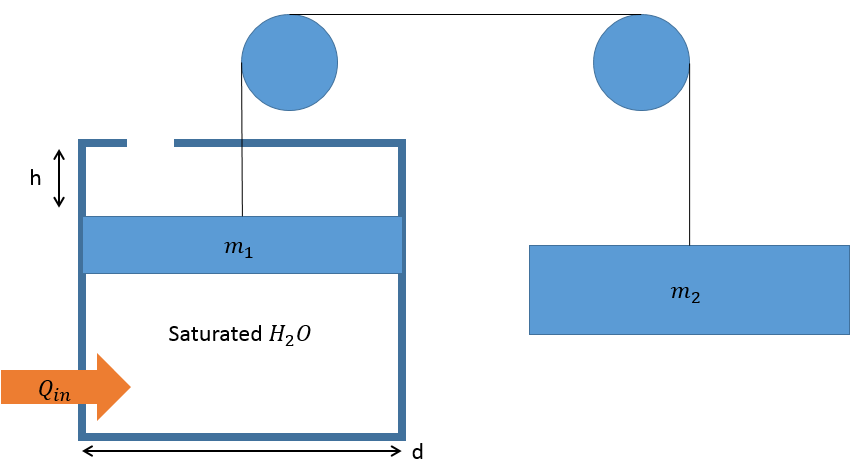
\includegraphics[scale=0.5]{Graphics/mass_system.PNG}\end{figure}

\emph{Tentative workthrough}: Assume the system is initially in equilibrium and that the piston is well-insulated (with the exception of the heat source, of course). (For the sake of being thorough we should also assume the string connecting the masses does not stretch and the pulleys are frictionless.) Then the pressure inside the cylinder is
$$p_{in} = p_{ext} + \frac{4(m_1-m_2)g}{\pi d^2}$$
Assume the process is quasi-static, which means it happens slowly and the interior of the piston rapidly adapts to changes in temperature or volume as heat is added. Thus we can assume the pressure inside the piston is constant throughout the process and
$$dH = \delta Q\to \Delta H = Q_{in}$$
Since we have saturated water we can express the enthalpy difference between the initial and final states as the enthalpy of vaporization times the mass of water vaporized, which can in turn be expressed in terms of a change in quality
$$\Delta H = m_{vap}h_{fg} = mh_{fg}\Delta x = Q_{in}$$
Similarly, we find the volume change of the the saturated water, which we require to equal to the volume displaced
$$\Delta V = mv_{fg}\Delta x = \frac{1}{4}\pi d^2h$$
Solving either expression for the change in quality and subsituting gives
\CenteredBoxed{Q_{in} = \frac{h_{fg}}{v_{fg}}\frac{1}{4}\pi d^2h}
Recall that phase changes are both constant pressure and constant temperature (see a $p-v$ diagram), so the (initial) temperature and pressure dependencies are hidding inside the $h_{fg}$ and $v_{fg}$ terms. Of course, this expression needs to be sanity checked against the overall quality $x_0+\Delta x \leq1$. If the calculated value for the final quality exceeds 1 then superheated gas data is needed to solve the problem.\\

\Problem{2} Write the concentration rate equations for each species (except $M$) in the below mechanism
\begin{align*}
A_2 + M &\leftrightharpoons A + A + M & (1)\\
B_2 + M &\leftrightharpoons AB + B & (2)
\end{align*}

\emph{Workthrough}:
$$\frac{d[A_2]}{dt} = -k_{1,f}[A_2][M] + k_{1,r}[A]^2[M]$$
$$\frac{d[B_2]}{dt} = -k_{2,f}[B_2][A] + k_{2,r}[AB][B] = -\frac{d[AB]}{dt} = -\frac{d[B]}{dt}$$
$$\frac{d[A]}{dt} = 2(k_{1,f}[A_2][M] - k_{1,r}[A]^2[M]) -k_{2,f}[B_2][A] + k_{2,r}[AB][B]$$

\emph{What happens when we apply partial equilibrium to the second reaction? What does that mean physically?} Applying partial equilibrium to the second reaction means the ratio of the forward and reverse rates is constant, and that constant is the equilibrium concentration coefficient
$$K_{C,2} = \frac{k_{2,f}}{k_{2,r}} = \frac{[AB][B]}{[B_2][A]}$$
This approximation is typically applied to energy-neutral reactions which achieve equilibrium rapidly, adapting quickly to changes in concentrations caused by other reactions.

\emph{What happens when we apply the steady state approximation to species A? What does that mean physically?} Applying the steady state approximation to $A$ means the $d[A]/dt\to0$, which reduces the last rate equation (above) to an algebraic one. This approximation is applied to species for which the production and destruction rates are approximately equal, though this does not imply the concentration of $A$ is constant.

\Problem{3} Consider the one-way reaction $A+B\to C$ with a reaction rate given by $RR = k[A][B]\exp\left(E_A/RT\right)$. Plot the concentration of products as a function of time for two conditions: $E_A/R <<T$ and $E_A/R >>T$.

\emph{Workthrough}:\\
Assuming the reaction is exothermic, the pressure is moderate, and the temperature is around typical combustion temperatures (maybe 1500K?), the first case will see the concentration of $C$ rise from the get-go and slowly taper off to its equilibrium concentration. The second case will have a prolonged induction period, then rise much like the first case to reach the equilibrium concentration.

\emph{Find an expression for the concentration of A as a function of time if the activation energy is zero and the initial concentrations of the reactants are equal.} The zero activation energy gives us
$$\frac{d[C]}{dt} = k[A](t)[B](t)$$
while the equal initial concentration condition gives
$$[A](t)=[B](t)\to\frac{d[C]}{dt} = k\left([A](t)\right)^2$$
We can also equate the production of $C$ with the destruction of $A$, giving us the ODE
$$\frac{d[A]}{dt} = -k\left([A](t)\right)^2$$
Separation of variables, integration, application of limits and some rearranging yields
\CenteredBoxed{[A](t) = \frac{[A]_0}{1+k[A]_0t}}

\emph{Find a suitable chemical time.} The chemical time is defined such that 
$$\frac{[A](\tau_{chem})}{[A]_0}=\frac{1}{e}$$
$$\frac{[A]_0/(1+k[A]_0\tau_{chem})}{[A]_0}=\frac{1}{e}$$
\CenteredBoxed{\tau_{chem} = \frac{e-1}{k[A]_0}\propto\frac{1}{k[A]_0}}

\Problem{4} Consider the dissociation reaction $CO_2\to CO+O$. Compare the \emph{initial} rates of $CO$ production at low and high pressures.\\

\emph{Workthrough}:\\
Break down the global reaction into a three step mechanism with an activated complex
\begin{align*}
CO_2 + M &\to CO_2^* + M & (1)\\
CO_2^* + M &\to CO_2 + M & (2)\\
CO_2^* &\to CO + O & (3)
\end{align*}
Then apply the steady state approximation to the activated complex, which allows us to reduce its rate equation as follows
$$\frac{d[CO_2^*]}{dt} = k_1[CO_2][M] - k_2[CO_2^*][M] - k_3[CO_2^*] = 0$$
$$[CO_2^*] = \frac{k_1[CO_2][M]}{k_2[M] + k_3}$$
Substitute this into the rate equation for $CO$ gives
$$\frac{d[CO]}{dt} = k_3[CO_2^*] = \frac{k_1k_3[CO_2][M]}{k_2[M] + k_3} = \frac{k_1[M]}{1+\frac{k_2}{k_3}[M]}[CO_2] = k_g[CO_2]$$
Now we employ $[M]\propto p$. At low pressures the denominator goes to 1 and the global reaction rate looks like $k_1[M]$, while at high pressures the second term in the denominator dominates and the global reaction rate looks like $k_1k_3/k_2$.

\Problem{5} Define chemical potential without an equation. What is it physically? Why does it matter?\\

Chemical potential is the free energy (or enthalpy) added to a system by adding one unit of a substance to it. Physically, it represents the additional capacity for work supplied by the added medium. It is important because it provides a general condition for equilibrium: minimization of the chemical potential.

\Problem{6} Show that the specific heats of a perfect gas are only functions of temperature\\

Start from the definition of chemical potential
$$\mu(p,T) = \hat g(p,T) = \hat h - T\hat s$$
$$\mu^0(T) + RT\ln(p) = \hat h - T\hat s$$
$$\mu^0(T) + RT\ln(p) = \hat h - T\left(\frac{d\mu^0}{dT} + R\ln(p)\right)$$
\CenteredBoxed{\hat h = \mu^0(T) + T\frac{d\mu^0}{dT}}
$$\hat u = \hat h - p\hat v = \hat h - RT$$
\CenteredBoxed{\hat u = \mu^0(T) + T\left(\frac{d\mu^0}{dT} + R\right)}

Mayer's relation is a direct consequence of these derivations
\CenteredBoxed{\hat c_p - \hat c_v = R}
This result can also be obtained from the compressibility coefficients
$$\alpha = \frac{1}{V}\PartialConst{V}{T}{p} = \frac{1}{T}$$
$$\kappa = \frac{-1}{V}\PartialConst{V}{p}{T} = \frac{1}{p}$$
\CenteredBoxed{\hat c_p - \hat c_v = \frac{T\alpha^2\hat v}{\kappa} = \frac{p\hat v}{T} = R}

\Problem{7} Two gases, $A$ and $B$, are contained in a well-insulated box, separated by an impermeable membrane. The temperature, pressure, moles of gas, and initial volumes are all known. The gases are allowed to mix and heat is removed from the system. Determine the final temperature and pressure, the change in entropy, and the change in Gibbs free energy.\\

\emph{Assumptions}: The gases are ideal and calorically perfect. The molar specific heats of the gases are known. The surroundings act as an isothermal resevoir at some known temperature $T_{ext}$.\\

The final temperature can be found by energy balance of the isolated system
$$n_A\hat c_{v_A}(T_f-T_A) + n_B\hat c_{v_B}(T_f-T_B) + Q_{out} = 0$$
\CenteredBoxed{T_f = \frac{-Q_{out} + n_A\hat c_{v_A}T_A + n_B\hat c_{v_B}T_B}{n_A\hat c_{v_A} + n_B\hat c_{v_B}}}
The final pressure can then be found by applying the ideal gas law
\CenteredBoxed{p_f = \frac{(n_A+n_B)RT_f}{V_A+V_B}}

The entropy generation can be found by breaking down the process into three processes: isochoric thermal equilibration, isothermal mechanical equilibration, and heat extraction. The general expression for the differential entropy is given for clarity.
$$ S = S(U,V) \to dS = \PartialConst{S}{U}{V}dU + \PartialConst{S}{V}{U}dV$$
$$dS = \frac{\partial Q}{T} + \frac{p}{T}dV = \frac{c_V}{T}dT + \frac{nR}{V}dV$$
The isochoric thermal equilibration (i.e. heat transfer across the impermeable membrane with $dV = 0$) gives
$$dS = dS_A + dS_B = \frac{\partial Q}{T}\Big|_A + \frac{\partial Q}{T}\Big|_{B}$$
Integration between the two states, recognizing that the heat transfered from one gas must go to the other gas and employing the calorically perfect assumption gives
$$\Delta S_{therm} = n_A\hat c_{V_A}\ln\left(\frac{T_{mix}}{T_A}\right) + n_B\hat c_{V_B}\ln\left(\frac{T_{mix}}{T_B}\right)$$
Now allow the gases to mix isothermally ($dT = 0$)
$$\Delta S_{mech} = n_AR_u\ln\left(\frac{V_f}{V_A}\right) + n_BR_u\ln\left(\frac{V_f}{V_B}\right)$$
Finally, extract heat from the system to the surroundings (exactly how this is achieved is not important), accounting for the entropy changes in both gases as well as in the resvoir.
$$\Delta S_{heat} = n_A\hat c_{V_A}\ln\left(\frac{T_f}{T_{mix}}\right) + n_B\hat c_{V_B}\ln\left(\frac{T_f}{T_{mix}}\right) + \frac{Q_{out}}{T_{ext}}$$
Put it all together to get the total entropy change
\begin{align*}
\Delta S =& \Delta S_{therm} + \Delta S_{mech} + \Delta S_{heat} \\
=& n_A\hat c_{V_A}\ln\left(\frac{T_{mix}}{T_A}\right) + n_B\hat c_{V_B}\ln\left(\frac{T_{mix}}{T_B}\right) + n_AR_u\ln\left(\frac{V_f}{V_A}\right)+ n_BR_u\ln\left(\frac{V_f}{V_B}\right) \\
& + n_A\hat c_{V_A}\ln\left(\frac{T_f}{T_{mix}}\right) + n_B\hat c_{V_B}\ln\left(\frac{T_f}{T_{mix}}\right) + \frac{Q_{out}}{T_{ext}}
\end{align*}

A shorthand approach to this would be to apply the $TdS$ relations to each gas independently, recognizing the rules of logarithms to simplify the expression
\CenteredBoxed{\Delta S = n_A\hat c_{V_A}\ln\left(\frac{T_f}{T_A}\right) + n_AR_u\ln\left(\frac{V_f}{V_A}\right) + n_B\hat c_{V_B}\ln\left(\frac{T_f}{T_B}\right) + n_BR_u\ln\left(\frac{V_f}{V_B}\right) + \frac{Q_{out}}{T_{ext}}}

The initial Gibbs free energy is the sum of the two gases which, applying the ideal gas assumption, is equal to the chemical potential times the number of moles
$$G_{sys,init} = G_A + G_B = n_A(\mu^0_A(T_A) + R_uT_A\ln(p_A)) + n_B(\mu^0_B(T_B)+R_uT_B\ln(p_B))$$
where it is assumed $\mu^0$ is taken at the reference pressure of 1 with units consistent with the units of the pressure term(s). After mixing, the temperatures of the gases change and the partial pressure of each gas may change. So the Gibbs function after mixing is given by
$$G_{sys,mixed} = G_A + G_B = n_A(\mu^0_A(T_f) + R_uT_f\ln(\chi_Ap_f)) + n_B(\mu^0_B(T_f) + R_uT_f\ln(\chi_Bp_f))$$
Thus the change in the Gibbs function between the starting and ending points of the whole process is
\begin{align*}
\Delta G_{sys} =& G_{sys,mixed} - G_{sys,init}\\
=& n_A(\mu^0_A(T_f) + R_uT_f\ln(\chi_Ap_f)) + n_B(\mu^0_B(T_f) + R_uT_f\ln(\chi_Bp_f))\\
&- \left(n_A(\mu^0_A(T_A) + R_uT_A\ln(p_A)) + n_B(\mu^0_B(T_B)+R_uT_B\ln(p_B))\right)
\end{align*} 

\Problem{8} How would you modify a premixed combustion process (i.e. hardware is fixed but properties are variable) when the fuel is switched from methane to decane?\\

You would want to increase the residence time and increase the inlet temperature. Increasing the residence time can be achieved by slowing down the mass flow rate of premixed fluid, while increasing the inlet temperature can be achieved by some preheating method. You would want to do this because decane is significantly heavier than methane; $C_{10}H_{22}$ for $n$-decane has a molar mass of $10\times12 + 22\times1 = 144$ vs $CH_4$ for methane which has a molar mass of 16. The higher mass means lower diffusivity, so it does not mix as readily with the rest of the fluid. This, in turn, limits the reaction rates (chemical kinetics). That limitation can be overcome by simply allowing more time for the reactions to happen and by increasing the temperature, which increases the overeall energy and the collision frequency. You may also want to shift the stoichiometry towards the slightly rich condition; this will increase the heat released by the reactions, which facilitates the overall process in a manner similar to increasing the inlet temperature.

\Problem{9} Write the (pressure) equilibrium constant for the reaction 
$$aA + bB \to cC$$

\CenteredBoxed{K_p = \frac{\chi_C^c}{\chi_A^a\chi_B^b}p^{(c-(a+b))}}

In general, is $K_p$ a function of pressure? Justify your answer.\\

$K_p$ is purely a function of temperature, even though pressure may show up on the right hand side of the above equation. The fact that it is purely a function of temperature can be seen by deriving $K_p$ from the chemical potential of the mixture. The physical manifestation of this independence is that $K_p$ does not itself respond to changes in pressure; the ratio of mole fractions, raised to the powers of the stoichiometric coefficients, will adjust as pressure is changed such that the above equation holds for a a given, fixed $K_p$ at a given, fixed temperature.

\Problem{10} Of constant volume and constant pressure combustion processes, which would have a higher final temperature? Why?\\

Constant volume combustion would have a higher temperature. The first law applied to an isolated mass of calorically perfect gases is
$$mc_VdT = \partial Q - pdV$$
$$mc_V\Delta T = Q_{chem} - p\Delta V$$
The work done by the gas in expanding at constant pressure takes up some of the energy released by chemical reactions, lessening the magnitude of the right hand side, thereby reducing the final temperature.

\Problem{11} Consider an isolated system of octane and air at stoichiometric proportions. The gases combust completely, so the system now contains only combustion products at the adiabatic flame temperature. Is this process reversible? Can it reverse spontaneously? What if the octane is replaced with methane, again at stoichiometric proportions? What if the gases are hydrogen and oxygen? What if the system were not isolated? Justify your answers.\\

\Problem{12} The cross section of a spherical vessel is shown below. The two hemispheres are initially at 1000 Kelvin and separated by an impermeable membrane. At time $t=0$ the membrane is removed and a spark goes off in the center. Draw and describe the flame for each of the following cases (1a, 1b, 2a, 2b, 3a, 3b):\\

\begin{minipage}{0.48\textwidth}
\begin{enumerate}
	\item Fuel is methane, oxidizer is air
	\item Fuel is methane, oxidizer is oxygen
	\item Fuel is hydrogen, oxidizer is oxygen
	\end{enumerate}
	
	\begin{enumerate}[label=\alph*.]
	\item (1) is pure fuel and (2) is pure oxidizer
	\item (1) is premixed fuel/oxidizer at $\Phi=0.7$ and (2) is premixed fuel/oxidizer at $\Phi=1.6$
	\end{enumerate}
\end{minipage}
\begin{minipage}{0.48\textwidth}
	\centering
	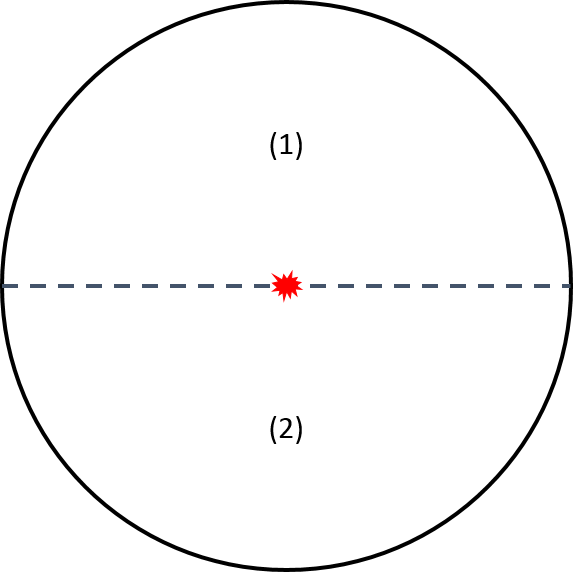
\includegraphics[width=0.7\textwidth]{Graphics/fuel_ox_sphere.PNG}
\end{minipage}

???????????????????????

\Problem{13}\\
\begin{minipage}{0.58\textwidth}
Consider the $n$-decane droplet array shown to the right. The initial temperature of the droplets is 175 Kelvin while the temperature of the surroundings (air) is 1500 Kelvin. Where will the flame start and how will it propagate? You may ignore gravity.
\end{minipage}
\begin{minipage}{0.38\textwidth}
\centering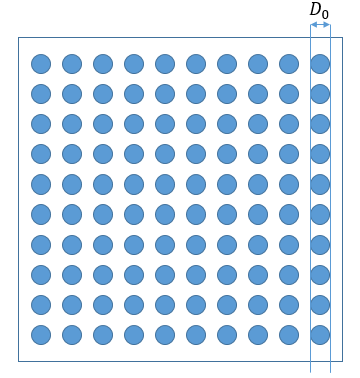
\includegraphics[width=0.7\textwidth]{Graphics/droplet_array.PNG}
\end{minipage}

\vspace{0.75cm}
The corners will ignite first, then the flame will propagate along the edges and eventually close over the top. The edges ignite first because they are the hottest. The droplets must evaporate before a diffusion flame can start, and evaporation takes energy; the droplets near the middle are all absorbing heat to evaporate and the cooling of the oxidizer around them increases the local induction time. The droplets on the end, however, experience less local temperature suppression and so have a less-impacted autoignition delay. Once the four corners go, the heat from those flames diffuses into the neighboring droplets; the edge droplets have an autoignition delay somewhere between those of the corners and the center. The flame then makes its way in towards the center from all edges as the necessary induction time is exceeded and heat from the flames diffuses inward.

Despite the importance of diffusion, this is not really a diffusion problem. The dominant effect is the heat required to evaporate the fuel droplets, and how that heat of vaporization impacts the induction time. Species diffusion becomes important once the flame is initiated, but not necessarily leading up to ignition.

\Problem{14} An insulated box is divided into three parts of equal volume. One part is filled with $N_A$ molecules of $A$, one part is filled with $N_B$ molecules of $B$, and the third part is a vacuum. Find
\begin{enumerate}[label = \alph*)]
\item The ratio of $\Omega$ after removal to $\Omega$ before removal of the partitions
\item The corresponding entropy change from statistical mechanics and classical thermodynamics
\end{enumerate}

Assume the two systems are at the same temperature and that the number of molecule sof each gas is reasonably high (i.e. we're talking about moles of gas here, not molecules). Then the volume of each species triples after the partitions are removed, and the expression for $\Omega$ for the most probable macrostate is
$$\ln(\Omega) \approx \ln(W_{max}) \approx N\ln(V)$$
so the ratio is
$$\frac{\Omega_2}{\Omega_1} = \frac{(V_2)^N}{(V_1)^N},\quad \Omega_{sys} = \Omega_A\Omega_B$$
$$\frac{\Omega_2}{\Omega_1}\Big|_{sys} = \left(\frac{\Omega_2}{\Omega_1}\Big|_A\right)\left(\frac{\Omega_2}{\Omega_1}\Big|_B\right)$$
$$\textrm{a})\ \frac{\Omega_2}{\Omega_1}\Big|_{sys} = 3^{(N_A+N_B)}$$

The entropy is related to $\Omega$ by
$$S = k\ln(\Omega)$$
where $k$ is the Boltzmann constant, so the corresponding entropy change from statistical therodynamics is
$$\textrm{b.1})\ S_2 - S_1 = k\ln\left(\frac{\Omega_2}{\Omega_1}\right) = k\ln\left(3^{(N_A+N_B)}\right)$$
while that from classical thermodynamics is
$$\textrm{b.2})\ S_2 - S_1 = \sum Nk\ln\left(\frac{V_2}{V_1}\right) = (N_A+N_B)k\ln(3)$$

The preceding equations which related $\Omega$ to $V$ and $N$ are
$$\ln(\Omega)\approx\ln(W_{max})$$
$$\ln(W_{max}) = N\left(1+\ln\left(\frac{Q}{N}\right)\right)+\beta E$$
$$Q=V\frac{(8\pi mkT)^{3/2}}{8h^3}$$
$$S = kN\ln\left(\frac{Q}{N}\right) + kN + \beta E$$
We assume we're dealing with very large numbers here, so we can make a lot of approximations and drop terms all over the place to arrive at the above solution.

\Problem{15} How would you find the entropy of a system in non-equilibrium?\\

We cannot use any of the Boltzmann statistics because they only apply to systems in equilibrium at high temperatures and moderate pressures. So go with Bose-Einstein or Fermi-Dirac statistics.

\Problem{16} Given the reaction $A+B\leftrightharpoons C$, how can you employ statistical mechanics to determine which way the reaction will proceed?\\

Boils down to maximizing $Q$ (how you can distribute energies)

\Problem{17} Is a plug flow reactor a good model for a premixed, 1D, laminar flame? What about counter-flow flames? Explain.\\

No to both. PFRs ignore axial diffusion, which is a critical component of laminar flame analysis, and the stretch effects in counter-flow flames would not be captured.

\Problem{18} How would you set up an analysis of an RQL (rich burn, quick mix, lean burn) combustor using the two reactor models? Explain.

\begin{figure}[h]\centering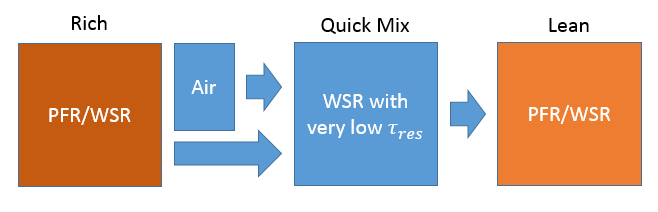
\includegraphics[width=0.7\textwidth]{Graphics/RQL_network.PNG}\end{figure}

Perfectly stirred reactors everywhere except for the (optional) burnout zone. This is based on a handful of papers on models of reacting flow CFD, where the PSR model provides a decent estimate of local conditions for large reactor networks. This type of system is typically very turbulent and is aided by recirculation zones for flame holding. It would be preferable to model the entire rich combustion zone as perfectly stirred because of these conditions, rather than as a premixed fluid simply flowing axially. More accurate models put equivalence ratio distributions over the network within the rich zone to emulate the stratified composition which is seen in fuel injection systems. The quick mix region is simply a dump of air, which will be a very turbulent process and we can simply the analysis by assuming no reactions; just an instantaneous, perfect mixing of air with the rich products. The lean combustion zone could possibly be modeled as a PFR, unless there was some new fuel injected into the system or a distribution of equivalence ratios was desired, in which case a network of PSRs would be more appropriate. In the burnout zone we can assume all the hot stuff is just flowing through with no real crazy stuff happening, so a plug flow reactor model is fine. (The burnout zone isn't even totally necessary so we could just leave it out.)

\Problem{19} Consider the reactor network created for Prolem 18 operating with propane as the fuel at 10 atmospheres with each combustion reactor having a volume of 1 $m^3$. The inlet temperature to the rich combustor follows a long-period sinusoid in time, while volumetric flow rate and composition remain constant ($\dot V = 5\ m^3/s$, $\phi=2.5$). The air at the inlet of the quick mix region is maintained at 1000 Kelvin. Enough air is added such that the equivalence ratio at the inlet of the lean zone would be 0.6 if no fuel burned in the rich zone. Sketch the mole fraction profiles of significant species at the exit of each combustion zone as a function of time. The temperature profile is given, in Kelvin, as
$$T_{in}(t) = 1000 + 200\cos(t/10),\quad t\in[0,20\pi]$$

Equivalence ratio has very little impact on autoignition delay. The residence time of each reactor, except the mixer, is 0.2 seconds, which is longer than the autoignition delay of propane at 1200 K. So initially there are rich combustion reactants coming out of the rich PSR. The exit temperature of the rich PSR will be around 2000 K. If we make the calorically perfect assumption and assuming the mixture specific heat is very close to that of nitrogen, the inlet temperature to the lean PSR will be around 1500 K. The lean mixture will continue to burn (autoignition delay has dropped since temperature has risen) and the outlet of the lean PSR will be lean products at around 2500 K. The mixture will then move towards equilibrium in the burnout zone, where carbon monoxide will form carbon dioxide and release heat, and nitrogen will react with excess oxygen to form nitric oxide at high temperatures via Zeldovich (or Extended Zeldovich). \\

The temperatures downstream will change with the inlet temperature to the rich PSR. The correlation is not 1:1, however, so the temperatures will decrease slightly less than that of the inlet. The rich mixture may not autoignite at the minimum temperature of 800 K but the fact that there was a flame in the reactor before then may prevent quenching (hysteresis). Propane has a decently high activation energy, in the ballpark of 400 kJ/mol (some sources suggest as high as 700 kJ/mol), so this could be an issue. Look at the two cases separately
\begin{itemize}
\Item{Extinguished} If the first PSR quenches then the whole system breaks down. The rich PSR would spit out a cold mixture almost identical to the inlet -- there may be a few reactions -- which would get mixed with air and then pushed into the lean PSR. The temperature going into the lean PSR would be slightly higher, probably around 900 K, since the incoming air is hot. This may or may not be high enough to ignite in the lean zone. Ignition in the lean combustor could be helped by some radical production inside the rich combustor. Going into the burnout zone, the mixture \emph{might} be able to autoignite. As the temperature at the inlet to the rich PSR goes back up, the lean zone will reignite first since it will be helped by radical production in the rich PSR. This will continue until the rich PSR reaches a temperature at which it can ignite, then regular operation resumes.
\Item{Not Extinguished} If the rich PSR does not quench then the reaction will simply not proceed as far at lower temperatures. The drop in temperature will be more gradual than it would be if it had quenched so it would be unlikely that the lean combustion zone would ever extinguish. Enough radicals and hot(ish) reactants would get pushed into the lean zone to sustain the combustion process. The burnout zone would then be largely unchanged aside from the somewhat reduced temperature. The whole system would then smoothly transition back to the initial conditions as the inlet temperature began to rise again.
\end{itemize}

\Problem{20}

\end{itemize}

\end{document}

